\documentclass[twoside]{book}

% Packages required by doxygen
\usepackage{calc}
\usepackage{doxygen}
\usepackage{graphicx}
\usepackage[utf8]{inputenc}
\usepackage{makeidx}
\usepackage{multicol}
\usepackage{multirow}
\usepackage{textcomp}
\usepackage[table]{xcolor}

% Font selection
\usepackage[T1]{fontenc}
\usepackage{mathptmx}
\usepackage[scaled=.90]{helvet}
\usepackage{courier}
\usepackage{amssymb}
\usepackage{sectsty}
\renewcommand{\familydefault}{\sfdefault}
\allsectionsfont{%
  \fontseries{bc}\selectfont%
  \color{darkgray}%
}
\renewcommand{\DoxyLabelFont}{%
  \fontseries{bc}\selectfont%
  \color{darkgray}%
}

% Page & text layout
\usepackage{geometry}
\geometry{%
  a4paper,%
  top=2.5cm,%
  bottom=2.5cm,%
  left=2.5cm,%
  right=2.5cm%
}
\tolerance=750
\hfuzz=15pt
\hbadness=750
\setlength{\emergencystretch}{15pt}
\setlength{\parindent}{0cm}
\setlength{\parskip}{0.2cm}
\makeatletter
\renewcommand{\paragraph}{%
  \@startsection{paragraph}{4}{0ex}{-1.0ex}{1.0ex}{%
    \normalfont\normalsize\bfseries\SS@parafont%
  }%
}
\renewcommand{\subparagraph}{%
  \@startsection{subparagraph}{5}{0ex}{-1.0ex}{1.0ex}{%
    \normalfont\normalsize\bfseries\SS@subparafont%
  }%
}
\makeatother

% Headers & footers
\usepackage{fancyhdr}
\pagestyle{fancyplain}
\fancyhead[LE]{\fancyplain{}{\bfseries\thepage}}
\fancyhead[CE]{\fancyplain{}{}}
\fancyhead[RE]{\fancyplain{}{\bfseries\leftmark}}
\fancyhead[LO]{\fancyplain{}{\bfseries\rightmark}}
\fancyhead[CO]{\fancyplain{}{}}
\fancyhead[RO]{\fancyplain{}{\bfseries\thepage}}
\fancyfoot[LE]{\fancyplain{}{}}
\fancyfoot[CE]{\fancyplain{}{}}
\fancyfoot[RE]{\fancyplain{}{\bfseries\scriptsize Generated on Thu Apr 10 2014 21\-:46\-:04 for K\-G\-E by Doxygen }}
\fancyfoot[LO]{\fancyplain{}{\bfseries\scriptsize Generated on Thu Apr 10 2014 21\-:46\-:04 for K\-G\-E by Doxygen }}
\fancyfoot[CO]{\fancyplain{}{}}
\fancyfoot[RO]{\fancyplain{}{}}
\renewcommand{\footrulewidth}{0.4pt}
\renewcommand{\chaptermark}[1]{%
  \markboth{#1}{}%
}
\renewcommand{\sectionmark}[1]{%
  \markright{\thesection\ #1}%
}

% Indices & bibliography
\usepackage{natbib}
\usepackage[titles]{tocloft}
\setcounter{tocdepth}{3}
\setcounter{secnumdepth}{5}
\makeindex

% Hyperlinks (required, but should be loaded last)
\usepackage{ifpdf}
\ifpdf
  \usepackage[pdftex,pagebackref=true]{hyperref}
\else
  \usepackage[ps2pdf,pagebackref=true]{hyperref}
\fi
\hypersetup{%
  colorlinks=true,%
  linkcolor=blue,%
  citecolor=blue,%
  unicode%
}

% Custom commands
\newcommand{\clearemptydoublepage}{%
  \newpage{\pagestyle{empty}\cleardoublepage}%
}


%===== C O N T E N T S =====

\begin{document}

% Titlepage & ToC
\hypersetup{pageanchor=false}
\pagenumbering{roman}
\begin{titlepage}
\vspace*{7cm}
\begin{center}%
{\Large K\-G\-E \\[1ex]\large 0 }\\
\vspace*{1cm}
{\large Generated by Doxygen 1.8.6}\\
\vspace*{0.5cm}
{\small Thu Apr 10 2014 21:46:04}\\
\end{center}
\end{titlepage}
\clearemptydoublepage
\tableofcontents
\clearemptydoublepage
\pagenumbering{arabic}
\hypersetup{pageanchor=true}

%--- Begin generated contents ---
\chapter{Hierarchical Index}
\section{Class Hierarchy}
This inheritance list is sorted roughly, but not completely, alphabetically\-:\begin{DoxyCompactList}
\item \contentsline{section}{K\-G\-E\-:\-:Audio\-Manager}{\pageref{class_k_g_e_1_1_audio_manager}}{}
\item \contentsline{section}{K\-G\-E\-:\-:T\-U\-I\-D$<$ T\-Object $>$\-:\-:Cached\-Reference}{\pageref{class_k_g_e_1_1_t_u_i_d_1_1_cached_reference}}{}
\item \contentsline{section}{K\-G\-E\-:\-:Class\-Factory$<$ root\-\_\-t $>$}{\pageref{class_k_g_e_1_1_class_factory}}{}
\item \contentsline{section}{K\-G\-E\-:\-:Class\-Factory1\-Arg$<$ root\-\_\-t, arg0\-\_\-t $>$}{\pageref{class_k_g_e_1_1_class_factory1_arg}}{}
\item \contentsline{section}{K\-G\-E\-:\-:Class\-Factory2\-Args$<$ root\-\_\-t, arg0\-\_\-t, arg1\-\_\-t $>$}{\pageref{class_k_g_e_1_1_class_factory2_args}}{}
\item \contentsline{section}{K\-G\-E\-:\-:Class\-Factory\-X\-M\-L$<$ root\-\_\-t $>$}{\pageref{class_k_g_e_1_1_class_factory_x_m_l}}{}
\item \contentsline{section}{K\-G\-E\-:\-:Class\-Factory\-X\-M\-L1\-Arg$<$ root\-\_\-t, arg0\-\_\-t $>$}{\pageref{class_k_g_e_1_1_class_factory_x_m_l1_arg}}{}
\item \contentsline{section}{K\-G\-E\-:\-:Event\-Signal$<$ owner\-\_\-t $>$\-:\-:Comparer}{\pageref{struct_k_g_e_1_1_event_signal_1_1_comparer}}{}
\item \contentsline{section}{K\-G\-E\-:\-:Component}{\pageref{class_k_g_e_1_1_component}}{}
\begin{DoxyCompactList}
\item \contentsline{section}{K\-G\-E\-:\-:Component\-Audio\-Clip}{\pageref{class_k_g_e_1_1_component_audio_clip}}{}
\item \contentsline{section}{K\-G\-E\-:\-:Component\-Button}{\pageref{class_k_g_e_1_1_component_button}}{}
\item \contentsline{section}{K\-G\-E\-:\-:Component\-Container}{\pageref{class_k_g_e_1_1_component_container}}{}
\begin{DoxyCompactList}
\item \contentsline{section}{K\-G\-E\-:\-:Component\-Collection}{\pageref{class_k_g_e_1_1_component_collection}}{}
\begin{DoxyCompactList}
\item \contentsline{section}{K\-G\-E\-:\-:Component\-State}{\pageref{class_k_g_e_1_1_component_state}}{}
\end{DoxyCompactList}
\item \contentsline{section}{K\-G\-E\-:\-:Component\-Composite}{\pageref{class_k_g_e_1_1_component_composite}}{}
\begin{DoxyCompactList}
\item \contentsline{section}{K\-G\-E\-:\-:Component\-State\-Machine}{\pageref{class_k_g_e_1_1_component_state_machine}}{}
\end{DoxyCompactList}
\end{DoxyCompactList}
\item \contentsline{section}{K\-G\-E\-:\-:Component\-Layer}{\pageref{class_k_g_e_1_1_component_layer}}{}
\begin{DoxyCompactList}
\item \contentsline{section}{K\-G\-E\-:\-:Component\-Camera\-Layer}{\pageref{class_k_g_e_1_1_component_camera_layer}}{}
\item \contentsline{section}{K\-G\-E\-:\-:Component\-Panel\-Layer}{\pageref{class_k_g_e_1_1_component_panel_layer}}{}
\item \contentsline{section}{K\-G\-E\-:\-:Component\-Window\-Layer}{\pageref{class_k_g_e_1_1_component_window_layer}}{}
\end{DoxyCompactList}
\item \contentsline{section}{K\-G\-E\-:\-:Component\-Music}{\pageref{class_k_g_e_1_1_component_music}}{}
\item \contentsline{section}{K\-G\-E\-:\-:Component\-Sprite}{\pageref{class_k_g_e_1_1_component_sprite}}{}
\item \contentsline{section}{K\-G\-E\-:\-:Component\-Updater}{\pageref{class_k_g_e_1_1_component_updater}}{}
\end{DoxyCompactList}
\item \contentsline{section}{K\-G\-E\-:\-:Create\-Functor1\-Arg\-Base$<$ root\-\_\-t, arg0\-\_\-t $>$}{\pageref{class_k_g_e_1_1_create_functor1_arg_base}}{}
\begin{DoxyCompactList}
\item \contentsline{section}{K\-G\-E\-:\-:Create\-Functor1\-Arg$<$ root\-\_\-t, this\-\_\-t, arg0\-\_\-t $>$}{\pageref{class_k_g_e_1_1_create_functor1_arg}}{}
\end{DoxyCompactList}
\item \contentsline{section}{K\-G\-E\-:\-:Create\-Functor2\-Args\-Base$<$ root\-\_\-t, arg0\-\_\-t, arg1\-\_\-t $>$}{\pageref{class_k_g_e_1_1_create_functor2_args_base}}{}
\begin{DoxyCompactList}
\item \contentsline{section}{K\-G\-E\-:\-:Create\-Functor2\-Args$<$ root\-\_\-t, this\-\_\-t, arg0\-\_\-t, arg1\-\_\-t $>$}{\pageref{class_k_g_e_1_1_create_functor2_args}}{}
\end{DoxyCompactList}
\item \contentsline{section}{K\-G\-E\-:\-:Create\-Functor\-Base$<$ root\-\_\-t $>$}{\pageref{class_k_g_e_1_1_create_functor_base}}{}
\begin{DoxyCompactList}
\item \contentsline{section}{K\-G\-E\-:\-:Create\-Functor$<$ root\-\_\-t, this\-\_\-t $>$}{\pageref{class_k_g_e_1_1_create_functor}}{}
\end{DoxyCompactList}
\item \contentsline{section}{K\-G\-E\-:\-:Create\-Functor\-X\-M\-L1\-Arg\-Base$<$ root\-\_\-t, arg0\-\_\-t $>$}{\pageref{class_k_g_e_1_1_create_functor_x_m_l1_arg_base}}{}
\begin{DoxyCompactList}
\item \contentsline{section}{K\-G\-E\-:\-:Create\-Functor\-X\-M\-L1\-Arg$<$ root\-\_\-t, this\-\_\-t, arg0\-\_\-t $>$}{\pageref{class_k_g_e_1_1_create_functor_x_m_l1_arg}}{}
\end{DoxyCompactList}
\item \contentsline{section}{K\-G\-E\-:\-:Create\-Functor\-X\-M\-L\-Base$<$ root\-\_\-t $>$}{\pageref{class_k_g_e_1_1_create_functor_x_m_l_base}}{}
\begin{DoxyCompactList}
\item \contentsline{section}{K\-G\-E\-:\-:Create\-Functor\-X\-M\-L$<$ root\-\_\-t, this\-\_\-t $>$}{\pageref{class_k_g_e_1_1_create_functor_x_m_l}}{}
\end{DoxyCompactList}
\item \contentsline{section}{K\-G\-E\-:\-:Data}{\pageref{class_k_g_e_1_1_data}}{}
\item \contentsline{section}{K\-G\-E\-:\-:Event$<$ owner\-\_\-t $>$}{\pageref{class_k_g_e_1_1_event}}{}
\item \contentsline{section}{K\-G\-E\-:\-:Event\-Signal$<$ owner\-\_\-t $>$}{\pageref{class_k_g_e_1_1_event_signal}}{}
\item \contentsline{section}{K\-G\-E\-:\-:Font\-Manager}{\pageref{class_k_g_e_1_1_font_manager}}{}
\item \contentsline{section}{K\-G\-E\-:\-:Hash}{\pageref{class_k_g_e_1_1_hash}}{}
\item \contentsline{section}{K\-G\-E\-:\-:Component\-Window\-Layer\-:\-:Hasher}{\pageref{struct_k_g_e_1_1_component_window_layer_1_1_hasher}}{}
\item \contentsline{section}{K\-G\-E\-:\-:Property\-:\-:Hasher}{\pageref{struct_k_g_e_1_1_property_1_1_hasher}}{}
\item \contentsline{section}{K\-G\-E\-:\-:Hash\-:\-:Hasher}{\pageref{struct_k_g_e_1_1_hash_1_1_hasher}}{}
\item \contentsline{section}{K\-G\-E\-:\-:T\-U\-I\-D$<$ T\-Object $>$\-:\-:Hasher}{\pageref{struct_k_g_e_1_1_t_u_i_d_1_1_hasher}}{}
\item \contentsline{section}{K\-G\-E\-:\-:T\-U\-I\-D$<$ T\-Object $>$\-:\-:Manager}{\pageref{struct_k_g_e_1_1_t_u_i_d_1_1_manager}}{}
\item \contentsline{section}{K\-G\-E\-:\-:Property}{\pageref{class_k_g_e_1_1_property}}{}
\begin{DoxyCompactList}
\item \contentsline{section}{K\-G\-E\-:\-:Property\-Data\-By\-Callback}{\pageref{class_k_g_e_1_1_property_data_by_callback}}{}
\item \contentsline{section}{K\-G\-E\-:\-:Property\-Data\-By\-Reference}{\pageref{class_k_g_e_1_1_property_data_by_reference}}{}
\item \contentsline{section}{K\-G\-E\-:\-:Property\-Data\-By\-Value}{\pageref{class_k_g_e_1_1_property_data_by_value}}{}
\item \contentsline{section}{K\-G\-E\-:\-:Property\-Typed\-By\-Callback$<$ type\-\_\-t $>$}{\pageref{class_k_g_e_1_1_property_typed_by_callback}}{}
\item \contentsline{section}{K\-G\-E\-:\-:Property\-Typed\-By\-Reference$<$ type\-\_\-t $>$}{\pageref{class_k_g_e_1_1_property_typed_by_reference}}{}
\item \contentsline{section}{K\-G\-E\-:\-:Property\-Typed\-By\-Value$<$ type\-\_\-t $>$}{\pageref{class_k_g_e_1_1_property_typed_by_value}}{}
\end{DoxyCompactList}
\item \contentsline{section}{K\-G\-E\-:\-:Sprite}{\pageref{class_k_g_e_1_1_sprite}}{}
\item \contentsline{section}{K\-G\-E\-:\-:Texture\-Manager}{\pageref{class_k_g_e_1_1_texture_manager}}{}
\item \contentsline{section}{K\-G\-E\-:\-:T\-U\-I\-D$<$ T\-Object $>$}{\pageref{class_k_g_e_1_1_t_u_i_d}}{}
\item \contentsline{section}{K\-G\-E\-:\-:T\-U\-I\-D$<$ K\-G\-E\-:\-:Component $>$}{\pageref{class_k_g_e_1_1_t_u_i_d}}{}
\item \contentsline{section}{K\-G\-E\-:\-:Vec2f}{\pageref{struct_k_g_e_1_1_vec2f}}{}
\item \contentsline{section}{K\-G\-E\-:\-:X\-M\-L\-Attribute\-Handler$<$ parent\-\_\-t $>$}{\pageref{class_k_g_e_1_1_x_m_l_attribute_handler}}{}
\item \contentsline{section}{K\-G\-E\-:\-:X\-M\-L\-Child\-Handler$<$ parent\-\_\-t $>$}{\pageref{class_k_g_e_1_1_x_m_l_child_handler}}{}
\item \contentsline{section}{K\-G\-E\-:\-:X\-M\-L\-Helpers}{\pageref{class_k_g_e_1_1_x_m_l_helpers}}{}
\item \contentsline{section}{K\-G\-E\-:\-:X\-M\-L\-Parser$<$ this\-\_\-t $>$}{\pageref{class_k_g_e_1_1_x_m_l_parser}}{}
\end{DoxyCompactList}

\chapter{Class Index}
\section{Class List}
Here are the classes, structs, unions and interfaces with brief descriptions\-:\begin{DoxyCompactList}
\item\contentsline{section}{\hyperlink{class_k_g_e_1_1_audio_manager}{K\-G\-E\-::\-Audio\-Manager} }{\pageref{class_k_g_e_1_1_audio_manager}}{}
\item\contentsline{section}{\hyperlink{class_k_g_e_1_1_t_u_i_d_1_1_cached_reference}{K\-G\-E\-::\-T\-U\-I\-D$<$ T\-Object $>$\-::\-Cached\-Reference} }{\pageref{class_k_g_e_1_1_t_u_i_d_1_1_cached_reference}}{}
\item\contentsline{section}{\hyperlink{class_k_g_e_1_1_class_factory}{K\-G\-E\-::\-Class\-Factory$<$ root\-\_\-t $>$} }{\pageref{class_k_g_e_1_1_class_factory}}{}
\item\contentsline{section}{\hyperlink{class_k_g_e_1_1_class_factory1_arg}{K\-G\-E\-::\-Class\-Factory1\-Arg$<$ root\-\_\-t, arg0\-\_\-t $>$} }{\pageref{class_k_g_e_1_1_class_factory1_arg}}{}
\item\contentsline{section}{\hyperlink{class_k_g_e_1_1_class_factory2_args}{K\-G\-E\-::\-Class\-Factory2\-Args$<$ root\-\_\-t, arg0\-\_\-t, arg1\-\_\-t $>$} }{\pageref{class_k_g_e_1_1_class_factory2_args}}{}
\item\contentsline{section}{\hyperlink{class_k_g_e_1_1_class_factory_x_m_l}{K\-G\-E\-::\-Class\-Factory\-X\-M\-L$<$ root\-\_\-t $>$} }{\pageref{class_k_g_e_1_1_class_factory_x_m_l}}{}
\item\contentsline{section}{\hyperlink{class_k_g_e_1_1_class_factory_x_m_l1_arg}{K\-G\-E\-::\-Class\-Factory\-X\-M\-L1\-Arg$<$ root\-\_\-t, arg0\-\_\-t $>$} }{\pageref{class_k_g_e_1_1_class_factory_x_m_l1_arg}}{}
\item\contentsline{section}{\hyperlink{struct_k_g_e_1_1_event_signal_1_1_comparer}{K\-G\-E\-::\-Event\-Signal$<$ owner\-\_\-t $>$\-::\-Comparer} }{\pageref{struct_k_g_e_1_1_event_signal_1_1_comparer}}{}
\item\contentsline{section}{\hyperlink{class_k_g_e_1_1_component}{K\-G\-E\-::\-Component} }{\pageref{class_k_g_e_1_1_component}}{}
\item\contentsline{section}{\hyperlink{class_k_g_e_1_1_component_audio_clip}{K\-G\-E\-::\-Component\-Audio\-Clip} }{\pageref{class_k_g_e_1_1_component_audio_clip}}{}
\item\contentsline{section}{\hyperlink{class_k_g_e_1_1_component_button}{K\-G\-E\-::\-Component\-Button} }{\pageref{class_k_g_e_1_1_component_button}}{}
\item\contentsline{section}{\hyperlink{class_k_g_e_1_1_component_camera_layer}{K\-G\-E\-::\-Component\-Camera\-Layer} }{\pageref{class_k_g_e_1_1_component_camera_layer}}{}
\item\contentsline{section}{\hyperlink{class_k_g_e_1_1_component_collection}{K\-G\-E\-::\-Component\-Collection} }{\pageref{class_k_g_e_1_1_component_collection}}{}
\item\contentsline{section}{\hyperlink{class_k_g_e_1_1_component_composite}{K\-G\-E\-::\-Component\-Composite} }{\pageref{class_k_g_e_1_1_component_composite}}{}
\item\contentsline{section}{\hyperlink{class_k_g_e_1_1_component_container}{K\-G\-E\-::\-Component\-Container} }{\pageref{class_k_g_e_1_1_component_container}}{}
\item\contentsline{section}{\hyperlink{class_k_g_e_1_1_component_layer}{K\-G\-E\-::\-Component\-Layer} }{\pageref{class_k_g_e_1_1_component_layer}}{}
\item\contentsline{section}{\hyperlink{class_k_g_e_1_1_component_music}{K\-G\-E\-::\-Component\-Music} }{\pageref{class_k_g_e_1_1_component_music}}{}
\item\contentsline{section}{\hyperlink{class_k_g_e_1_1_component_panel_layer}{K\-G\-E\-::\-Component\-Panel\-Layer} }{\pageref{class_k_g_e_1_1_component_panel_layer}}{}
\item\contentsline{section}{\hyperlink{class_k_g_e_1_1_component_sprite}{K\-G\-E\-::\-Component\-Sprite} }{\pageref{class_k_g_e_1_1_component_sprite}}{}
\item\contentsline{section}{\hyperlink{class_k_g_e_1_1_component_state}{K\-G\-E\-::\-Component\-State} }{\pageref{class_k_g_e_1_1_component_state}}{}
\item\contentsline{section}{\hyperlink{class_k_g_e_1_1_component_state_machine}{K\-G\-E\-::\-Component\-State\-Machine} }{\pageref{class_k_g_e_1_1_component_state_machine}}{}
\item\contentsline{section}{\hyperlink{class_k_g_e_1_1_component_updater}{K\-G\-E\-::\-Component\-Updater} }{\pageref{class_k_g_e_1_1_component_updater}}{}
\item\contentsline{section}{\hyperlink{class_k_g_e_1_1_component_window_layer}{K\-G\-E\-::\-Component\-Window\-Layer} }{\pageref{class_k_g_e_1_1_component_window_layer}}{}
\item\contentsline{section}{\hyperlink{class_k_g_e_1_1_create_functor}{K\-G\-E\-::\-Create\-Functor$<$ root\-\_\-t, this\-\_\-t $>$} }{\pageref{class_k_g_e_1_1_create_functor}}{}
\item\contentsline{section}{\hyperlink{class_k_g_e_1_1_create_functor1_arg}{K\-G\-E\-::\-Create\-Functor1\-Arg$<$ root\-\_\-t, this\-\_\-t, arg0\-\_\-t $>$} }{\pageref{class_k_g_e_1_1_create_functor1_arg}}{}
\item\contentsline{section}{\hyperlink{class_k_g_e_1_1_create_functor1_arg_base}{K\-G\-E\-::\-Create\-Functor1\-Arg\-Base$<$ root\-\_\-t, arg0\-\_\-t $>$} }{\pageref{class_k_g_e_1_1_create_functor1_arg_base}}{}
\item\contentsline{section}{\hyperlink{class_k_g_e_1_1_create_functor2_args}{K\-G\-E\-::\-Create\-Functor2\-Args$<$ root\-\_\-t, this\-\_\-t, arg0\-\_\-t, arg1\-\_\-t $>$} }{\pageref{class_k_g_e_1_1_create_functor2_args}}{}
\item\contentsline{section}{\hyperlink{class_k_g_e_1_1_create_functor2_args_base}{K\-G\-E\-::\-Create\-Functor2\-Args\-Base$<$ root\-\_\-t, arg0\-\_\-t, arg1\-\_\-t $>$} }{\pageref{class_k_g_e_1_1_create_functor2_args_base}}{}
\item\contentsline{section}{\hyperlink{class_k_g_e_1_1_create_functor_base}{K\-G\-E\-::\-Create\-Functor\-Base$<$ root\-\_\-t $>$} }{\pageref{class_k_g_e_1_1_create_functor_base}}{}
\item\contentsline{section}{\hyperlink{class_k_g_e_1_1_create_functor_x_m_l}{K\-G\-E\-::\-Create\-Functor\-X\-M\-L$<$ root\-\_\-t, this\-\_\-t $>$} }{\pageref{class_k_g_e_1_1_create_functor_x_m_l}}{}
\item\contentsline{section}{\hyperlink{class_k_g_e_1_1_create_functor_x_m_l1_arg}{K\-G\-E\-::\-Create\-Functor\-X\-M\-L1\-Arg$<$ root\-\_\-t, this\-\_\-t, arg0\-\_\-t $>$} }{\pageref{class_k_g_e_1_1_create_functor_x_m_l1_arg}}{}
\item\contentsline{section}{\hyperlink{class_k_g_e_1_1_create_functor_x_m_l1_arg_base}{K\-G\-E\-::\-Create\-Functor\-X\-M\-L1\-Arg\-Base$<$ root\-\_\-t, arg0\-\_\-t $>$} }{\pageref{class_k_g_e_1_1_create_functor_x_m_l1_arg_base}}{}
\item\contentsline{section}{\hyperlink{class_k_g_e_1_1_create_functor_x_m_l_base}{K\-G\-E\-::\-Create\-Functor\-X\-M\-L\-Base$<$ root\-\_\-t $>$} }{\pageref{class_k_g_e_1_1_create_functor_x_m_l_base}}{}
\item\contentsline{section}{\hyperlink{class_k_g_e_1_1_data}{K\-G\-E\-::\-Data} }{\pageref{class_k_g_e_1_1_data}}{}
\item\contentsline{section}{\hyperlink{class_k_g_e_1_1_event}{K\-G\-E\-::\-Event$<$ owner\-\_\-t $>$} }{\pageref{class_k_g_e_1_1_event}}{}
\item\contentsline{section}{\hyperlink{class_k_g_e_1_1_event_signal}{K\-G\-E\-::\-Event\-Signal$<$ owner\-\_\-t $>$} }{\pageref{class_k_g_e_1_1_event_signal}}{}
\item\contentsline{section}{\hyperlink{class_k_g_e_1_1_font_manager}{K\-G\-E\-::\-Font\-Manager} }{\pageref{class_k_g_e_1_1_font_manager}}{}
\item\contentsline{section}{\hyperlink{class_k_g_e_1_1_hash}{K\-G\-E\-::\-Hash} }{\pageref{class_k_g_e_1_1_hash}}{}
\item\contentsline{section}{\hyperlink{struct_k_g_e_1_1_component_window_layer_1_1_hasher}{K\-G\-E\-::\-Component\-Window\-Layer\-::\-Hasher} }{\pageref{struct_k_g_e_1_1_component_window_layer_1_1_hasher}}{}
\item\contentsline{section}{\hyperlink{struct_k_g_e_1_1_property_1_1_hasher}{K\-G\-E\-::\-Property\-::\-Hasher} }{\pageref{struct_k_g_e_1_1_property_1_1_hasher}}{}
\item\contentsline{section}{\hyperlink{struct_k_g_e_1_1_hash_1_1_hasher}{K\-G\-E\-::\-Hash\-::\-Hasher} }{\pageref{struct_k_g_e_1_1_hash_1_1_hasher}}{}
\item\contentsline{section}{\hyperlink{struct_k_g_e_1_1_t_u_i_d_1_1_hasher}{K\-G\-E\-::\-T\-U\-I\-D$<$ T\-Object $>$\-::\-Hasher} }{\pageref{struct_k_g_e_1_1_t_u_i_d_1_1_hasher}}{}
\item\contentsline{section}{\hyperlink{struct_k_g_e_1_1_t_u_i_d_1_1_manager}{K\-G\-E\-::\-T\-U\-I\-D$<$ T\-Object $>$\-::\-Manager} }{\pageref{struct_k_g_e_1_1_t_u_i_d_1_1_manager}}{}
\item\contentsline{section}{\hyperlink{class_k_g_e_1_1_property}{K\-G\-E\-::\-Property} }{\pageref{class_k_g_e_1_1_property}}{}
\item\contentsline{section}{\hyperlink{class_k_g_e_1_1_property_data_by_callback}{K\-G\-E\-::\-Property\-Data\-By\-Callback} }{\pageref{class_k_g_e_1_1_property_data_by_callback}}{}
\item\contentsline{section}{\hyperlink{class_k_g_e_1_1_property_data_by_reference}{K\-G\-E\-::\-Property\-Data\-By\-Reference} }{\pageref{class_k_g_e_1_1_property_data_by_reference}}{}
\item\contentsline{section}{\hyperlink{class_k_g_e_1_1_property_data_by_value}{K\-G\-E\-::\-Property\-Data\-By\-Value} }{\pageref{class_k_g_e_1_1_property_data_by_value}}{}
\item\contentsline{section}{\hyperlink{class_k_g_e_1_1_property_typed_by_callback}{K\-G\-E\-::\-Property\-Typed\-By\-Callback$<$ type\-\_\-t $>$} }{\pageref{class_k_g_e_1_1_property_typed_by_callback}}{}
\item\contentsline{section}{\hyperlink{class_k_g_e_1_1_property_typed_by_reference}{K\-G\-E\-::\-Property\-Typed\-By\-Reference$<$ type\-\_\-t $>$} }{\pageref{class_k_g_e_1_1_property_typed_by_reference}}{}
\item\contentsline{section}{\hyperlink{class_k_g_e_1_1_property_typed_by_value}{K\-G\-E\-::\-Property\-Typed\-By\-Value$<$ type\-\_\-t $>$} }{\pageref{class_k_g_e_1_1_property_typed_by_value}}{}
\item\contentsline{section}{\hyperlink{class_k_g_e_1_1_sprite}{K\-G\-E\-::\-Sprite} }{\pageref{class_k_g_e_1_1_sprite}}{}
\item\contentsline{section}{\hyperlink{class_k_g_e_1_1_texture_manager}{K\-G\-E\-::\-Texture\-Manager} }{\pageref{class_k_g_e_1_1_texture_manager}}{}
\item\contentsline{section}{\hyperlink{class_k_g_e_1_1_t_u_i_d}{K\-G\-E\-::\-T\-U\-I\-D$<$ T\-Object $>$} }{\pageref{class_k_g_e_1_1_t_u_i_d}}{}
\item\contentsline{section}{\hyperlink{struct_k_g_e_1_1_vec2f}{K\-G\-E\-::\-Vec2f} }{\pageref{struct_k_g_e_1_1_vec2f}}{}
\item\contentsline{section}{\hyperlink{class_k_g_e_1_1_x_m_l_attribute_handler}{K\-G\-E\-::\-X\-M\-L\-Attribute\-Handler$<$ parent\-\_\-t $>$} }{\pageref{class_k_g_e_1_1_x_m_l_attribute_handler}}{}
\item\contentsline{section}{\hyperlink{class_k_g_e_1_1_x_m_l_child_handler}{K\-G\-E\-::\-X\-M\-L\-Child\-Handler$<$ parent\-\_\-t $>$} }{\pageref{class_k_g_e_1_1_x_m_l_child_handler}}{}
\item\contentsline{section}{\hyperlink{class_k_g_e_1_1_x_m_l_helpers}{K\-G\-E\-::\-X\-M\-L\-Helpers} }{\pageref{class_k_g_e_1_1_x_m_l_helpers}}{}
\item\contentsline{section}{\hyperlink{class_k_g_e_1_1_x_m_l_parser}{K\-G\-E\-::\-X\-M\-L\-Parser$<$ this\-\_\-t $>$} }{\pageref{class_k_g_e_1_1_x_m_l_parser}}{}
\end{DoxyCompactList}

\chapter{Class Documentation}
\hypertarget{class_k_g_e_1_1_audio_manager}{\section{K\-G\-E\-:\-:Audio\-Manager Class Reference}
\label{class_k_g_e_1_1_audio_manager}\index{K\-G\-E\-::\-Audio\-Manager@{K\-G\-E\-::\-Audio\-Manager}}
}
\subsection*{Public Member Functions}
\begin{DoxyCompactItemize}
\item 
\hypertarget{class_k_g_e_1_1_audio_manager_a6bf2dc211229a40466f0540914d346ce}{sf\-::\-Sound\-Buffer $\ast$ {\bfseries Load\-Sound\-Buffer} (const std\-::string \&sz\-File\-Name)}\label{class_k_g_e_1_1_audio_manager_a6bf2dc211229a40466f0540914d346ce}

\item 
\hypertarget{class_k_g_e_1_1_audio_manager_ac0c0d798d67b3b44e9426e852dcad6d6}{sf\-::\-Sound\-Buffer $\ast$ {\bfseries Get\-Sound\-Buffer} (const \hyperlink{class_k_g_e_1_1_hash}{Hash} \&x\-Hash)}\label{class_k_g_e_1_1_audio_manager_ac0c0d798d67b3b44e9426e852dcad6d6}

\item 
\hypertarget{class_k_g_e_1_1_audio_manager_ae3026354c1c161f6be0e9b0316d54fd0}{void {\bfseries Release\-Sound\-Buffer} (const \hyperlink{class_k_g_e_1_1_hash}{Hash} \&x\-Hash)}\label{class_k_g_e_1_1_audio_manager_ae3026354c1c161f6be0e9b0316d54fd0}

\item 
\hypertarget{class_k_g_e_1_1_audio_manager_a1bb38460c179762402de6e5bd29878bc}{void {\bfseries Release\-Sound\-Buffer} (sf\-::\-Sound\-Buffer $\ast$px\-Sound\-Buffer)}\label{class_k_g_e_1_1_audio_manager_a1bb38460c179762402de6e5bd29878bc}

\item 
\hypertarget{class_k_g_e_1_1_audio_manager_abdd1f5cfc90ab01999ae4a4f3b96dc4c}{sf\-::\-Music $\ast$ {\bfseries Load\-Music} (const std\-::string \&sz\-File\-Name)}\label{class_k_g_e_1_1_audio_manager_abdd1f5cfc90ab01999ae4a4f3b96dc4c}

\item 
\hypertarget{class_k_g_e_1_1_audio_manager_a31cd2ed12aa70872ba01470e577f5f7c}{sf\-::\-Music $\ast$ {\bfseries Get\-Music} (const \hyperlink{class_k_g_e_1_1_hash}{Hash} \&x\-Hash)}\label{class_k_g_e_1_1_audio_manager_a31cd2ed12aa70872ba01470e577f5f7c}

\item 
\hypertarget{class_k_g_e_1_1_audio_manager_adf67d324fc7c9d71e35c6b7e2a1ef5db}{void {\bfseries Release\-Music} (const \hyperlink{class_k_g_e_1_1_hash}{Hash} \&x\-Hash)}\label{class_k_g_e_1_1_audio_manager_adf67d324fc7c9d71e35c6b7e2a1ef5db}

\item 
\hypertarget{class_k_g_e_1_1_audio_manager_a3702028b53e65c39eef6cdd5c2e00350}{void {\bfseries Release\-Music} (sf\-::\-Music $\ast$px\-Music)}\label{class_k_g_e_1_1_audio_manager_a3702028b53e65c39eef6cdd5c2e00350}

\end{DoxyCompactItemize}
\subsection*{Static Public Member Functions}
\begin{DoxyCompactItemize}
\item 
\hypertarget{class_k_g_e_1_1_audio_manager_a36f4d0f8cf9965e964dda470e50739f8}{static \hyperlink{class_k_g_e_1_1_audio_manager}{Audio\-Manager} \& {\bfseries Get} ()}\label{class_k_g_e_1_1_audio_manager_a36f4d0f8cf9965e964dda470e50739f8}

\end{DoxyCompactItemize}
\subsection*{Protected Attributes}
\begin{DoxyCompactItemize}
\item 
\hypertarget{class_k_g_e_1_1_audio_manager_ab527929d483d470f8dc40a63a4197c50}{soundcollection\-\_\-t {\bfseries m\-\_\-x\-Sound\-List}}\label{class_k_g_e_1_1_audio_manager_ab527929d483d470f8dc40a63a4197c50}

\item 
\hypertarget{class_k_g_e_1_1_audio_manager_accb62181d1b08212b64cec52c5aaba1d}{musiccollection\-\_\-t {\bfseries m\-\_\-x\-Music\-List}}\label{class_k_g_e_1_1_audio_manager_accb62181d1b08212b64cec52c5aaba1d}

\end{DoxyCompactItemize}


The documentation for this class was generated from the following files\-:\begin{DoxyCompactItemize}
\item 
C\-:/\-Users/\-Vit/\-Documents/\-Git\-Hub/\-K\-G\-E/\-K\-G\-E/\-Core/\-Resources/Audio\-Manager.\-hpp\item 
C\-:/\-Users/\-Vit/\-Documents/\-Git\-Hub/\-K\-G\-E/\-K\-G\-E/\-Core/\-Resources/Audio\-Manager.\-cpp\end{DoxyCompactItemize}

\hypertarget{class_k_g_e_1_1_t_u_i_d_1_1_cached_reference}{\section{K\-G\-E\-:\-:T\-U\-I\-D$<$ T\-Object $>$\-:\-:Cached\-Reference Class Reference}
\label{class_k_g_e_1_1_t_u_i_d_1_1_cached_reference}\index{K\-G\-E\-::\-T\-U\-I\-D$<$ T\-Object $>$\-::\-Cached\-Reference@{K\-G\-E\-::\-T\-U\-I\-D$<$ T\-Object $>$\-::\-Cached\-Reference}}
}
\subsection*{Public Member Functions}
\begin{DoxyCompactItemize}
\item 
\hypertarget{class_k_g_e_1_1_t_u_i_d_1_1_cached_reference_a57a5ea445a11f21b9e9543f7fd6ca3bd}{{\bfseries Cached\-Reference} (const \hyperlink{class_k_g_e_1_1_t_u_i_d}{T\-U\-I\-D} \&x\-Target)}\label{class_k_g_e_1_1_t_u_i_d_1_1_cached_reference_a57a5ea445a11f21b9e9543f7fd6ca3bd}

\item 
\hypertarget{class_k_g_e_1_1_t_u_i_d_1_1_cached_reference_a280be533d28e96b6df4a64b0e5244930}{{\bfseries Cached\-Reference} (const \hyperlink{class_k_g_e_1_1_t_u_i_d_1_1_cached_reference}{Cached\-Reference} \&x\-Copy)}\label{class_k_g_e_1_1_t_u_i_d_1_1_cached_reference_a280be533d28e96b6df4a64b0e5244930}

\item 
\hypertarget{class_k_g_e_1_1_t_u_i_d_1_1_cached_reference_a3b79bbdc9eeba5636443491c51c5ca6b}{void {\bfseries Set\-Target} (const \hyperlink{class_k_g_e_1_1_t_u_i_d}{T\-U\-I\-D} \&x\-Target)}\label{class_k_g_e_1_1_t_u_i_d_1_1_cached_reference_a3b79bbdc9eeba5636443491c51c5ca6b}

\item 
\hypertarget{class_k_g_e_1_1_t_u_i_d_1_1_cached_reference_a890c066db5400b75f6c5eb6e4ef4b032}{void {\bfseries Set\-Target} (u\-\_\-int u\-Target)}\label{class_k_g_e_1_1_t_u_i_d_1_1_cached_reference_a890c066db5400b75f6c5eb6e4ef4b032}

\item 
\hypertarget{class_k_g_e_1_1_t_u_i_d_1_1_cached_reference_a8a81fcf570352af92e85598339edfb28}{void {\bfseries Clear} ()}\label{class_k_g_e_1_1_t_u_i_d_1_1_cached_reference_a8a81fcf570352af92e85598339edfb28}

\item 
\hypertarget{class_k_g_e_1_1_t_u_i_d_1_1_cached_reference_ac5a30e7a46bc0594f473edc7083ffbe4}{T\-Object $\ast$ {\bfseries operator()} () const }\label{class_k_g_e_1_1_t_u_i_d_1_1_cached_reference_ac5a30e7a46bc0594f473edc7083ffbe4}

\end{DoxyCompactItemize}
\subsection*{Protected Attributes}
\begin{DoxyCompactItemize}
\item 
\hypertarget{class_k_g_e_1_1_t_u_i_d_1_1_cached_reference_a4497f5facd874ed1ff1f9c115fc605df}{u\-\_\-int {\bfseries m\-\_\-u\-Target\-T\-U\-I\-D}}\label{class_k_g_e_1_1_t_u_i_d_1_1_cached_reference_a4497f5facd874ed1ff1f9c115fc605df}

\item 
\hypertarget{class_k_g_e_1_1_t_u_i_d_1_1_cached_reference_a71adfa89d5b57a23bef5eba267e245db}{T\-Object $\ast$ {\bfseries m\-\_\-px\-Target\-Object}}\label{class_k_g_e_1_1_t_u_i_d_1_1_cached_reference_a71adfa89d5b57a23bef5eba267e245db}

\end{DoxyCompactItemize}


The documentation for this class was generated from the following file\-:\begin{DoxyCompactItemize}
\item 
C\-:/\-Users/\-Vit/\-Documents/\-Git\-Hub/\-K\-G\-E/\-K\-G\-E/\-Core/\-Data/T\-U\-I\-D.\-hpp\end{DoxyCompactItemize}

\hypertarget{class_k_g_e_1_1_class_factory}{\section{K\-G\-E\-:\-:Class\-Factory$<$ root\-\_\-t $>$ Class Template Reference}
\label{class_k_g_e_1_1_class_factory}\index{K\-G\-E\-::\-Class\-Factory$<$ root\-\_\-t $>$@{K\-G\-E\-::\-Class\-Factory$<$ root\-\_\-t $>$}}
}
\subsection*{Public Types}
\begin{DoxyCompactItemize}
\item 
\hypertarget{class_k_g_e_1_1_class_factory_af5f63e0339440a3eb0189b222b778f9b}{typedef \hyperlink{class_k_g_e_1_1_create_functor_base}{Create\-Functor\-Base}$<$ root\-\_\-t $>$ {\bfseries Functor}}\label{class_k_g_e_1_1_class_factory_af5f63e0339440a3eb0189b222b778f9b}

\end{DoxyCompactItemize}
\subsection*{Public Member Functions}
\begin{DoxyCompactItemize}
\item 
\hypertarget{class_k_g_e_1_1_class_factory_a20ea1b618be5137db62f37b4a5533a9e}{void {\bfseries Register} (const \hyperlink{class_k_g_e_1_1_hash}{Hash} \&x\-Hash, \hyperlink{class_k_g_e_1_1_create_functor_base}{Functor} $\ast$px\-Create\-Functor)}\label{class_k_g_e_1_1_class_factory_a20ea1b618be5137db62f37b4a5533a9e}

\item 
\hypertarget{class_k_g_e_1_1_class_factory_a43c905623c97d5984b232b533a0ebb22}{root\-\_\-t $\ast$ {\bfseries Create} (const \hyperlink{class_k_g_e_1_1_hash}{Hash} \&x\-Hash)}\label{class_k_g_e_1_1_class_factory_a43c905623c97d5984b232b533a0ebb22}

\end{DoxyCompactItemize}
\subsection*{Static Public Member Functions}
\begin{DoxyCompactItemize}
\item 
\hypertarget{class_k_g_e_1_1_class_factory_a12d3ef7f2deeecc39f5a336cabc0abad}{static \hyperlink{class_k_g_e_1_1_class_factory}{Class\-Factory} \& {\bfseries Get} ()}\label{class_k_g_e_1_1_class_factory_a12d3ef7f2deeecc39f5a336cabc0abad}

\end{DoxyCompactItemize}
\subsection*{Protected Types}
\begin{DoxyCompactItemize}
\item 
\hypertarget{class_k_g_e_1_1_class_factory_a686d27d678009cf5522e2e0b1d20e372}{typedef unordered\-\_\-map$<$ \hyperlink{class_k_g_e_1_1_hash}{Hash}, \\*
\hyperlink{class_k_g_e_1_1_create_functor_base}{Functor} $\ast$, \hyperlink{struct_k_g_e_1_1_hash_1_1_hasher}{Hash\-::\-Hasher} $>$ {\bfseries Functor\-Collection}}\label{class_k_g_e_1_1_class_factory_a686d27d678009cf5522e2e0b1d20e372}

\item 
\hypertarget{class_k_g_e_1_1_class_factory_a516fcb574774a7888109ca72872a2d22}{typedef pair$<$ \hyperlink{class_k_g_e_1_1_hash}{Hash}, \hyperlink{class_k_g_e_1_1_create_functor_base}{Functor} $\ast$ $>$ {\bfseries Functor\-Pair}}\label{class_k_g_e_1_1_class_factory_a516fcb574774a7888109ca72872a2d22}

\end{DoxyCompactItemize}
\subsection*{Protected Attributes}
\begin{DoxyCompactItemize}
\item 
\hypertarget{class_k_g_e_1_1_class_factory_a9e8321e0c6ea9d341aa07ce509e0cca1}{Functor\-Collection {\bfseries m\-\_\-x\-Create\-Functors}}\label{class_k_g_e_1_1_class_factory_a9e8321e0c6ea9d341aa07ce509e0cca1}

\end{DoxyCompactItemize}


The documentation for this class was generated from the following file\-:\begin{DoxyCompactItemize}
\item 
C\-:/\-Users/\-Vit/\-Documents/\-Git\-Hub/\-K\-G\-E/\-K\-G\-E/\-Core/\-Class\-Capabilities/Class\-Factory.\-hpp\end{DoxyCompactItemize}

\hypertarget{class_k_g_e_1_1_class_factory1_arg}{\section{K\-G\-E\-:\-:Class\-Factory1\-Arg$<$ root\-\_\-t, arg0\-\_\-t $>$ Class Template Reference}
\label{class_k_g_e_1_1_class_factory1_arg}\index{K\-G\-E\-::\-Class\-Factory1\-Arg$<$ root\-\_\-t, arg0\-\_\-t $>$@{K\-G\-E\-::\-Class\-Factory1\-Arg$<$ root\-\_\-t, arg0\-\_\-t $>$}}
}
\subsection*{Public Types}
\begin{DoxyCompactItemize}
\item 
\hypertarget{class_k_g_e_1_1_class_factory1_arg_a117754bb49ee78af4ef3afe6f1a027f5}{typedef \hyperlink{class_k_g_e_1_1_create_functor1_arg_base}{Create\-Functor1\-Arg\-Base}\\*
$<$ root\-\_\-t, arg0\-\_\-t $>$ {\bfseries Functor}}\label{class_k_g_e_1_1_class_factory1_arg_a117754bb49ee78af4ef3afe6f1a027f5}

\end{DoxyCompactItemize}
\subsection*{Public Member Functions}
\begin{DoxyCompactItemize}
\item 
\hypertarget{class_k_g_e_1_1_class_factory1_arg_adc88101022205a659013c7baec4c763c}{void {\bfseries Register} (const \hyperlink{class_k_g_e_1_1_hash}{Hash} \&x\-Hash, \hyperlink{class_k_g_e_1_1_create_functor1_arg_base}{Functor} $\ast$px\-Create\-Functor)}\label{class_k_g_e_1_1_class_factory1_arg_adc88101022205a659013c7baec4c763c}

\item 
\hypertarget{class_k_g_e_1_1_class_factory1_arg_a8b6263282af1aa3f01807f7336a1567d}{root\-\_\-t $\ast$ {\bfseries Create} (const \hyperlink{class_k_g_e_1_1_hash}{Hash} \&x\-Hash, arg0\-\_\-t x\-Arg0)}\label{class_k_g_e_1_1_class_factory1_arg_a8b6263282af1aa3f01807f7336a1567d}

\end{DoxyCompactItemize}
\subsection*{Static Public Member Functions}
\begin{DoxyCompactItemize}
\item 
\hypertarget{class_k_g_e_1_1_class_factory1_arg_aaf4b86eafc6993010e01267805b78217}{static \hyperlink{class_k_g_e_1_1_class_factory1_arg}{Class\-Factory1\-Arg} \& {\bfseries Get} ()}\label{class_k_g_e_1_1_class_factory1_arg_aaf4b86eafc6993010e01267805b78217}

\end{DoxyCompactItemize}
\subsection*{Protected Types}
\begin{DoxyCompactItemize}
\item 
\hypertarget{class_k_g_e_1_1_class_factory1_arg_a16355da66b450d04fc8f501d935c28b6}{typedef unordered\-\_\-map$<$ \hyperlink{class_k_g_e_1_1_hash}{Hash}, \\*
\hyperlink{class_k_g_e_1_1_create_functor1_arg_base}{Functor} $\ast$, \hyperlink{struct_k_g_e_1_1_hash_1_1_hasher}{Hash\-::\-Hasher} $>$ {\bfseries Functor\-Collection}}\label{class_k_g_e_1_1_class_factory1_arg_a16355da66b450d04fc8f501d935c28b6}

\item 
\hypertarget{class_k_g_e_1_1_class_factory1_arg_ac69a5fc5053bdc8c689fab5e6732f7e4}{typedef pair$<$ \hyperlink{class_k_g_e_1_1_hash}{Hash}, \hyperlink{class_k_g_e_1_1_create_functor1_arg_base}{Functor} $\ast$ $>$ {\bfseries Functor\-Pair}}\label{class_k_g_e_1_1_class_factory1_arg_ac69a5fc5053bdc8c689fab5e6732f7e4}

\end{DoxyCompactItemize}
\subsection*{Protected Attributes}
\begin{DoxyCompactItemize}
\item 
\hypertarget{class_k_g_e_1_1_class_factory1_arg_a5159715d70d7cbe3e43a3d3d87be9d4b}{Functor\-Collection {\bfseries m\-\_\-x\-Create\-Functors}}\label{class_k_g_e_1_1_class_factory1_arg_a5159715d70d7cbe3e43a3d3d87be9d4b}

\end{DoxyCompactItemize}


The documentation for this class was generated from the following file\-:\begin{DoxyCompactItemize}
\item 
C\-:/\-Users/\-Vit/\-Documents/\-Git\-Hub/\-K\-G\-E/\-K\-G\-E/\-Core/\-Class\-Capabilities/Class\-Factory.\-hpp\end{DoxyCompactItemize}

\hypertarget{class_k_g_e_1_1_class_factory2_args}{\section{K\-G\-E\-:\-:Class\-Factory2\-Args$<$ root\-\_\-t, arg0\-\_\-t, arg1\-\_\-t $>$ Class Template Reference}
\label{class_k_g_e_1_1_class_factory2_args}\index{K\-G\-E\-::\-Class\-Factory2\-Args$<$ root\-\_\-t, arg0\-\_\-t, arg1\-\_\-t $>$@{K\-G\-E\-::\-Class\-Factory2\-Args$<$ root\-\_\-t, arg0\-\_\-t, arg1\-\_\-t $>$}}
}
\subsection*{Public Types}
\begin{DoxyCompactItemize}
\item 
\hypertarget{class_k_g_e_1_1_class_factory2_args_a57e2d8f95d00bac9e0153914ece1a33f}{typedef \hyperlink{class_k_g_e_1_1_create_functor2_args_base}{Create\-Functor2\-Args\-Base}\\*
$<$ root\-\_\-t, arg0\-\_\-t, arg1\-\_\-t $>$ {\bfseries Functor}}\label{class_k_g_e_1_1_class_factory2_args_a57e2d8f95d00bac9e0153914ece1a33f}

\end{DoxyCompactItemize}
\subsection*{Public Member Functions}
\begin{DoxyCompactItemize}
\item 
\hypertarget{class_k_g_e_1_1_class_factory2_args_a9462d75be206de86f848a2ffac32ca9c}{void {\bfseries Register} (const \hyperlink{class_k_g_e_1_1_hash}{Hash} \&x\-Hash, \hyperlink{class_k_g_e_1_1_create_functor2_args_base}{Functor} $\ast$px\-Create\-Functor)}\label{class_k_g_e_1_1_class_factory2_args_a9462d75be206de86f848a2ffac32ca9c}

\item 
\hypertarget{class_k_g_e_1_1_class_factory2_args_a1545f76275ec6b20776c5665f4d86745}{root\-\_\-t $\ast$ {\bfseries Create} (const \hyperlink{class_k_g_e_1_1_hash}{Hash} \&x\-Hash, arg0\-\_\-t x\-Arg0, arg1\-\_\-t x\-Arg1)}\label{class_k_g_e_1_1_class_factory2_args_a1545f76275ec6b20776c5665f4d86745}

\end{DoxyCompactItemize}
\subsection*{Static Public Member Functions}
\begin{DoxyCompactItemize}
\item 
\hypertarget{class_k_g_e_1_1_class_factory2_args_a354edd08806f83cbfe732a5a96dc53bd}{static \hyperlink{class_k_g_e_1_1_class_factory2_args}{Class\-Factory2\-Args} \& {\bfseries Get} ()}\label{class_k_g_e_1_1_class_factory2_args_a354edd08806f83cbfe732a5a96dc53bd}

\end{DoxyCompactItemize}
\subsection*{Protected Types}
\begin{DoxyCompactItemize}
\item 
\hypertarget{class_k_g_e_1_1_class_factory2_args_a99dfb7d72fef5a633d8e97e0760bedb5}{typedef unordered\-\_\-map$<$ \hyperlink{class_k_g_e_1_1_hash}{Hash}, \\*
\hyperlink{class_k_g_e_1_1_create_functor2_args_base}{Functor} $\ast$, \hyperlink{struct_k_g_e_1_1_hash_1_1_hasher}{Hash\-::\-Hasher} $>$ {\bfseries Functor\-Collection}}\label{class_k_g_e_1_1_class_factory2_args_a99dfb7d72fef5a633d8e97e0760bedb5}

\item 
\hypertarget{class_k_g_e_1_1_class_factory2_args_a362f3a23fcae57dd759f3ce0ca51748f}{typedef pair$<$ \hyperlink{class_k_g_e_1_1_hash}{Hash}, \hyperlink{class_k_g_e_1_1_create_functor2_args_base}{Functor} $\ast$ $>$ {\bfseries Functor\-Pair}}\label{class_k_g_e_1_1_class_factory2_args_a362f3a23fcae57dd759f3ce0ca51748f}

\end{DoxyCompactItemize}
\subsection*{Protected Attributes}
\begin{DoxyCompactItemize}
\item 
\hypertarget{class_k_g_e_1_1_class_factory2_args_a89a86de8ce76810a893056c6e8054cca}{Functor\-Collection {\bfseries m\-\_\-x\-Create\-Functors}}\label{class_k_g_e_1_1_class_factory2_args_a89a86de8ce76810a893056c6e8054cca}

\end{DoxyCompactItemize}


The documentation for this class was generated from the following file\-:\begin{DoxyCompactItemize}
\item 
C\-:/\-Users/\-Vit/\-Documents/\-Git\-Hub/\-K\-G\-E/\-K\-G\-E/\-Core/\-Class\-Capabilities/Class\-Factory.\-hpp\end{DoxyCompactItemize}

\hypertarget{class_k_g_e_1_1_class_factory_x_m_l}{\section{K\-G\-E\-:\-:Class\-Factory\-X\-M\-L$<$ root\-\_\-t $>$ Class Template Reference}
\label{class_k_g_e_1_1_class_factory_x_m_l}\index{K\-G\-E\-::\-Class\-Factory\-X\-M\-L$<$ root\-\_\-t $>$@{K\-G\-E\-::\-Class\-Factory\-X\-M\-L$<$ root\-\_\-t $>$}}
}
\subsection*{Public Types}
\begin{DoxyCompactItemize}
\item 
\hypertarget{class_k_g_e_1_1_class_factory_x_m_l_ae739bb8562789f755b760b7a6241c258}{typedef \hyperlink{class_k_g_e_1_1_create_functor_x_m_l_base}{Create\-Functor\-X\-M\-L\-Base}\\*
$<$ root\-\_\-t $>$ {\bfseries Functor}}\label{class_k_g_e_1_1_class_factory_x_m_l_ae739bb8562789f755b760b7a6241c258}

\end{DoxyCompactItemize}
\subsection*{Public Member Functions}
\begin{DoxyCompactItemize}
\item 
\hypertarget{class_k_g_e_1_1_class_factory_x_m_l_a59baec4c0ba02b14e2a2942e238298a8}{void {\bfseries Register} (const \hyperlink{class_k_g_e_1_1_hash}{Hash} \&x\-Hash, \hyperlink{class_k_g_e_1_1_create_functor_x_m_l_base}{Functor} $\ast$px\-Create\-Functor)}\label{class_k_g_e_1_1_class_factory_x_m_l_a59baec4c0ba02b14e2a2942e238298a8}

\item 
\hypertarget{class_k_g_e_1_1_class_factory_x_m_l_a66329c64c8efb1d8c8669b79a70d07dc}{root\-\_\-t $\ast$ {\bfseries Create} (xml\-\_\-node$<$ char $>$ \&x\-Node)}\label{class_k_g_e_1_1_class_factory_x_m_l_a66329c64c8efb1d8c8669b79a70d07dc}

\end{DoxyCompactItemize}
\subsection*{Static Public Member Functions}
\begin{DoxyCompactItemize}
\item 
\hypertarget{class_k_g_e_1_1_class_factory_x_m_l_a625e5a1817369af4e3011da2c70708a8}{static \hyperlink{class_k_g_e_1_1_class_factory_x_m_l}{Class\-Factory\-X\-M\-L} \& {\bfseries Get} ()}\label{class_k_g_e_1_1_class_factory_x_m_l_a625e5a1817369af4e3011da2c70708a8}

\end{DoxyCompactItemize}
\subsection*{Protected Types}
\begin{DoxyCompactItemize}
\item 
\hypertarget{class_k_g_e_1_1_class_factory_x_m_l_a8c2e979f222d637c6f1b1fc4d54408d4}{typedef unordered\-\_\-map$<$ \hyperlink{class_k_g_e_1_1_hash}{Hash}, \\*
\hyperlink{class_k_g_e_1_1_create_functor_x_m_l_base}{Functor} $\ast$, \hyperlink{struct_k_g_e_1_1_hash_1_1_hasher}{Hash\-::\-Hasher} $>$ {\bfseries Functor\-Collection}}\label{class_k_g_e_1_1_class_factory_x_m_l_a8c2e979f222d637c6f1b1fc4d54408d4}

\item 
\hypertarget{class_k_g_e_1_1_class_factory_x_m_l_a3da822ce3d5b8e475557d1ec428670e5}{typedef pair$<$ \hyperlink{class_k_g_e_1_1_hash}{Hash}, \hyperlink{class_k_g_e_1_1_create_functor_x_m_l_base}{Functor} $\ast$ $>$ {\bfseries Functor\-Pair}}\label{class_k_g_e_1_1_class_factory_x_m_l_a3da822ce3d5b8e475557d1ec428670e5}

\end{DoxyCompactItemize}
\subsection*{Protected Attributes}
\begin{DoxyCompactItemize}
\item 
\hypertarget{class_k_g_e_1_1_class_factory_x_m_l_a0a800b89a0dda3594fbec22bb278c6eb}{Functor\-Collection {\bfseries m\-\_\-x\-Create\-Functors}}\label{class_k_g_e_1_1_class_factory_x_m_l_a0a800b89a0dda3594fbec22bb278c6eb}

\end{DoxyCompactItemize}


The documentation for this class was generated from the following file\-:\begin{DoxyCompactItemize}
\item 
C\-:/\-Users/\-Vit/\-Documents/\-Git\-Hub/\-K\-G\-E/\-K\-G\-E/\-Core/\-Class\-Capabilities/Class\-Factory.\-hpp\end{DoxyCompactItemize}

\hypertarget{class_k_g_e_1_1_class_factory_x_m_l1_arg}{\section{K\-G\-E\-:\-:Class\-Factory\-X\-M\-L1\-Arg$<$ root\-\_\-t, arg0\-\_\-t $>$ Class Template Reference}
\label{class_k_g_e_1_1_class_factory_x_m_l1_arg}\index{K\-G\-E\-::\-Class\-Factory\-X\-M\-L1\-Arg$<$ root\-\_\-t, arg0\-\_\-t $>$@{K\-G\-E\-::\-Class\-Factory\-X\-M\-L1\-Arg$<$ root\-\_\-t, arg0\-\_\-t $>$}}
}
\subsection*{Public Types}
\begin{DoxyCompactItemize}
\item 
\hypertarget{class_k_g_e_1_1_class_factory_x_m_l1_arg_aebbdbabc79044d6cc51e180944a7a723}{typedef \\*
\hyperlink{class_k_g_e_1_1_create_functor_x_m_l1_arg_base}{Create\-Functor\-X\-M\-L1\-Arg\-Base}\\*
$<$ root\-\_\-t, arg0\-\_\-t $>$ {\bfseries Functor}}\label{class_k_g_e_1_1_class_factory_x_m_l1_arg_aebbdbabc79044d6cc51e180944a7a723}

\end{DoxyCompactItemize}
\subsection*{Public Member Functions}
\begin{DoxyCompactItemize}
\item 
\hypertarget{class_k_g_e_1_1_class_factory_x_m_l1_arg_a8c3d004e79ea696f4166c0cd66e5c3ca}{void {\bfseries Register} (const \hyperlink{class_k_g_e_1_1_hash}{Hash} \&x\-Hash, \hyperlink{class_k_g_e_1_1_create_functor_x_m_l1_arg_base}{Functor} $\ast$px\-Create\-Functor)}\label{class_k_g_e_1_1_class_factory_x_m_l1_arg_a8c3d004e79ea696f4166c0cd66e5c3ca}

\item 
\hypertarget{class_k_g_e_1_1_class_factory_x_m_l1_arg_aa2be3450995ec528547b3eb1eb579a13}{root\-\_\-t $\ast$ {\bfseries Create} (xml\-\_\-node$<$ char $>$ \&x\-Node, arg0\-\_\-t x\-Arg0)}\label{class_k_g_e_1_1_class_factory_x_m_l1_arg_aa2be3450995ec528547b3eb1eb579a13}

\end{DoxyCompactItemize}
\subsection*{Static Public Member Functions}
\begin{DoxyCompactItemize}
\item 
\hypertarget{class_k_g_e_1_1_class_factory_x_m_l1_arg_ae2f04e58952b885d516fe7033b916866}{static \hyperlink{class_k_g_e_1_1_class_factory_x_m_l1_arg}{Class\-Factory\-X\-M\-L1\-Arg} \& {\bfseries Get} ()}\label{class_k_g_e_1_1_class_factory_x_m_l1_arg_ae2f04e58952b885d516fe7033b916866}

\end{DoxyCompactItemize}
\subsection*{Protected Types}
\begin{DoxyCompactItemize}
\item 
\hypertarget{class_k_g_e_1_1_class_factory_x_m_l1_arg_abbc8c1bd5d4426d461453b15a1d164dd}{typedef unordered\-\_\-map$<$ \hyperlink{class_k_g_e_1_1_hash}{Hash}, \\*
\hyperlink{class_k_g_e_1_1_create_functor_x_m_l1_arg_base}{Functor} $\ast$, \hyperlink{struct_k_g_e_1_1_hash_1_1_hasher}{Hash\-::\-Hasher} $>$ {\bfseries Functor\-Collection}}\label{class_k_g_e_1_1_class_factory_x_m_l1_arg_abbc8c1bd5d4426d461453b15a1d164dd}

\item 
\hypertarget{class_k_g_e_1_1_class_factory_x_m_l1_arg_a1357038a93d60245c7229723b4781a70}{typedef pair$<$ \hyperlink{class_k_g_e_1_1_hash}{Hash}, \hyperlink{class_k_g_e_1_1_create_functor_x_m_l1_arg_base}{Functor} $\ast$ $>$ {\bfseries Functor\-Pair}}\label{class_k_g_e_1_1_class_factory_x_m_l1_arg_a1357038a93d60245c7229723b4781a70}

\end{DoxyCompactItemize}
\subsection*{Protected Attributes}
\begin{DoxyCompactItemize}
\item 
\hypertarget{class_k_g_e_1_1_class_factory_x_m_l1_arg_a85dcc7854ef4e925c57a8c1442817b0c}{Functor\-Collection {\bfseries m\-\_\-x\-Create\-Functors}}\label{class_k_g_e_1_1_class_factory_x_m_l1_arg_a85dcc7854ef4e925c57a8c1442817b0c}

\end{DoxyCompactItemize}


The documentation for this class was generated from the following file\-:\begin{DoxyCompactItemize}
\item 
C\-:/\-Users/\-Vit/\-Documents/\-Git\-Hub/\-K\-G\-E/\-K\-G\-E/\-Core/\-Class\-Capabilities/Class\-Factory.\-hpp\end{DoxyCompactItemize}

\hypertarget{struct_k_g_e_1_1_event_signal_1_1_comparer}{\section{K\-G\-E\-:\-:Event\-Signal$<$ owner\-\_\-t $>$\-:\-:Comparer Struct Reference}
\label{struct_k_g_e_1_1_event_signal_1_1_comparer}\index{K\-G\-E\-::\-Event\-Signal$<$ owner\-\_\-t $>$\-::\-Comparer@{K\-G\-E\-::\-Event\-Signal$<$ owner\-\_\-t $>$\-::\-Comparer}}
}
\subsection*{Public Member Functions}
\begin{DoxyCompactItemize}
\item 
\hypertarget{struct_k_g_e_1_1_event_signal_1_1_comparer_aaf14e9a03427f2d39d74eb9a9caed840}{bool {\bfseries operator()} (const \hyperlink{class_k_g_e_1_1_event_signal}{Event\-Signal} $\ast$px\-L\-H\-S, const \hyperlink{class_k_g_e_1_1_event_signal}{Event\-Signal} $\ast$px\-R\-H\-S) const }\label{struct_k_g_e_1_1_event_signal_1_1_comparer_aaf14e9a03427f2d39d74eb9a9caed840}

\end{DoxyCompactItemize}


The documentation for this struct was generated from the following file\-:\begin{DoxyCompactItemize}
\item 
C\-:/\-Users/\-Vit/\-Documents/\-Git\-Hub/\-K\-G\-E/\-K\-G\-E/\-Core/\-Class\-Capabilities/Event\-Signal.\-hpp\end{DoxyCompactItemize}

\hypertarget{class_k_g_e_1_1_component}{\section{K\-G\-E\-:\-:Component Class Reference}
\label{class_k_g_e_1_1_component}\index{K\-G\-E\-::\-Component@{K\-G\-E\-::\-Component}}
}
Inheritance diagram for K\-G\-E\-:\-:Component\-:\begin{figure}[H]
\begin{center}
\leavevmode
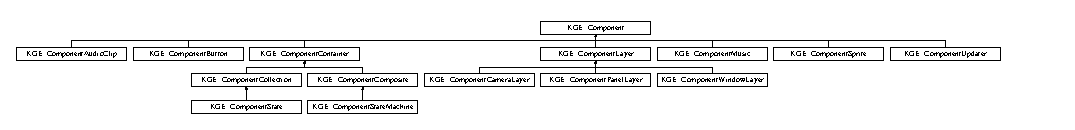
\includegraphics[height=1.303083cm]{class_k_g_e_1_1_component}
\end{center}
\end{figure}
\subsection*{Public Types}
\begin{DoxyCompactItemize}
\item 
enum {\bfseries State} \{ {\bfseries Unset}, 
{\bfseries Active}, 
{\bfseries Dormant}, 
{\bfseries Destroyed}
 \}
\end{DoxyCompactItemize}
\subsection*{Public Member Functions}
\begin{DoxyCompactItemize}
\item 
\hypertarget{class_k_g_e_1_1_component_af85894a43348979804943c44095a6bc7}{{\bfseries Component} (\hyperlink{class_k_g_e_1_1_t_u_i_d}{T\-U\-I\-D}$<$ \hyperlink{class_k_g_e_1_1_component}{Component} $>$\-::Cached\-Reference x\-Parent)}\label{class_k_g_e_1_1_component_af85894a43348979804943c44095a6bc7}

\item 
\hypertarget{class_k_g_e_1_1_component_a33359d0c293e91dc1cd6445d11c09878}{{\bfseries Component} (xml\-\_\-node$<$ char $>$ \&x\-Node, \hyperlink{class_k_g_e_1_1_t_u_i_d}{T\-U\-I\-D}$<$ \hyperlink{class_k_g_e_1_1_component}{Component} $>$\-::Cached\-Reference x\-Parent)}\label{class_k_g_e_1_1_component_a33359d0c293e91dc1cd6445d11c09878}

\item 
\hypertarget{class_k_g_e_1_1_component_a3126cb2bd30ca80dbd4ce228aafc4072}{void {\bfseries On\-Event\-By\-Path} (const char $\ast$sz\-Path, eventparams\-\_\-t \&x\-Event\-Parameters)}\label{class_k_g_e_1_1_component_a3126cb2bd30ca80dbd4ce228aafc4072}

\item 
\hypertarget{class_k_g_e_1_1_component_a5667460ebc2a72c2b75d26e754926948}{\hyperlink{class_k_g_e_1_1_event}{Event}$<$ \hyperlink{class_k_g_e_1_1_component}{Component} $>$ $\ast$ {\bfseries Get\-Event\-By\-Path} (const char $\ast$sz\-Path)}\label{class_k_g_e_1_1_component_a5667460ebc2a72c2b75d26e754926948}

\item 
\hypertarget{class_k_g_e_1_1_component_af8a56a0f8035731eb8c54af5f1a1d50b}{\hyperlink{class_k_g_e_1_1_data}{Data} {\bfseries Get\-Property\-By\-Path} (const char $\ast$sz\-Path)}\label{class_k_g_e_1_1_component_af8a56a0f8035731eb8c54af5f1a1d50b}

\item 
\hypertarget{class_k_g_e_1_1_component_a8263ad0b576478b77eb0aa06eb3e0c82}{{\footnotesize template$<$class T\-Y\-P\-E\-\_\-\-T $>$ }\\T\-Y\-P\-E\-\_\-\-T $\ast$ {\bfseries Get\-Parent\-By\-Type} ()}\label{class_k_g_e_1_1_component_a8263ad0b576478b77eb0aa06eb3e0c82}

\item 
\hypertarget{class_k_g_e_1_1_component_ad20a2b1caaacf735fdd4dfc1332fbb08}{\hyperlink{class_k_g_e_1_1_component}{Component} $\ast$ {\bfseries Get\-Parent\-By\-Type} (const \hyperlink{class_k_g_e_1_1_hash}{Hash} \&x\-Type)}\label{class_k_g_e_1_1_component_ad20a2b1caaacf735fdd4dfc1332fbb08}

\item 
\hypertarget{class_k_g_e_1_1_component_a110fe64c4ae028a0d17f6c887be4753d}{\hyperlink{class_k_g_e_1_1_component}{Component} $\ast$ {\bfseries Get\-Parent\-By\-Name} (const \hyperlink{class_k_g_e_1_1_hash}{Hash} \&x\-Name)}\label{class_k_g_e_1_1_component_a110fe64c4ae028a0d17f6c887be4753d}

\item 
\hypertarget{class_k_g_e_1_1_component_ae97d8043655d44bf23efaf34ad07ac09}{virtual \hyperlink{class_k_g_e_1_1_component_updater}{Component\-Updater} $\ast$ {\bfseries Get\-Updater} ()}\label{class_k_g_e_1_1_component_ae97d8043655d44bf23efaf34ad07ac09}

\item 
\hypertarget{class_k_g_e_1_1_component_a85db1628f659dd44ef0933e4cbcdea78}{virtual \hyperlink{class_k_g_e_1_1_component_layer}{Component\-Layer} $\ast$ {\bfseries Get\-Layer} ()}\label{class_k_g_e_1_1_component_a85db1628f659dd44ef0933e4cbcdea78}

\item 
\hypertarget{class_k_g_e_1_1_component_a9c2c70f08da7fe7d0e94c4eee1ef2c37}{virtual float {\bfseries Get\-Priority} ()}\label{class_k_g_e_1_1_component_a9c2c70f08da7fe7d0e94c4eee1ef2c37}

\item 
\hypertarget{class_k_g_e_1_1_component_aaa31b2c83d8981fa4f7ba0bd2a496062}{const \hyperlink{class_k_g_e_1_1_hash}{Hash} \& {\bfseries Get\-Name} ()}\label{class_k_g_e_1_1_component_aaa31b2c83d8981fa4f7ba0bd2a496062}

\item 
\hypertarget{class_k_g_e_1_1_component_a08ef1943824c6ed24a1f022e5b70e03a}{State {\bfseries Get\-State} ()}\label{class_k_g_e_1_1_component_a08ef1943824c6ed24a1f022e5b70e03a}

\item 
\hypertarget{class_k_g_e_1_1_component_ae79e0c0cb5109749dd62e3f4bcac3dd2}{virtual bool {\bfseries Is\-Composite} () const }\label{class_k_g_e_1_1_component_ae79e0c0cb5109749dd62e3f4bcac3dd2}

\item 
\hypertarget{class_k_g_e_1_1_component_a7587279caf161378404ecaa0ed7582e4}{virtual bool {\bfseries Is\-Collection} () const }\label{class_k_g_e_1_1_component_a7587279caf161378404ecaa0ed7582e4}

\item 
\hypertarget{class_k_g_e_1_1_component_ad18fab646887afea15a21144ea59d5d4}{virtual void {\bfseries On\-Create} (eventparams\-\_\-t \&x\-Event\-Parameters)}\label{class_k_g_e_1_1_component_ad18fab646887afea15a21144ea59d5d4}

\item 
\hypertarget{class_k_g_e_1_1_component_a345806a8602e41e704691f22cfe01dcf}{virtual void {\bfseries On\-Activate} (eventparams\-\_\-t \&x\-Event\-Parameters)}\label{class_k_g_e_1_1_component_a345806a8602e41e704691f22cfe01dcf}

\item 
\hypertarget{class_k_g_e_1_1_component_a9c89319c75b7c01ff870019458f35e68}{virtual void {\bfseries On\-Deactivate} (eventparams\-\_\-t \&x\-Event\-Parameters)}\label{class_k_g_e_1_1_component_a9c89319c75b7c01ff870019458f35e68}

\item 
\hypertarget{class_k_g_e_1_1_component_a55fb5a2d3d18b32c06e5d09ede54e4a9}{virtual void {\bfseries On\-Destroy} (eventparams\-\_\-t \&x\-Event\-Parameters)}\label{class_k_g_e_1_1_component_a55fb5a2d3d18b32c06e5d09ede54e4a9}

\item 
\hypertarget{class_k_g_e_1_1_component_a465878aacc4cc7a260e87379a3803850}{virtual bool {\bfseries Handle\-Input} (sf\-::\-Event \&x\-Event, sf\-::\-Window $\ast$px\-Window)}\label{class_k_g_e_1_1_component_a465878aacc4cc7a260e87379a3803850}

\item 
\hypertarget{class_k_g_e_1_1_component_a4e038c491b68883684e135d4fa9431c4}{virtual void {\bfseries Render} (sf\-::\-Render\-Target \&x\-Target)}\label{class_k_g_e_1_1_component_a4e038c491b68883684e135d4fa9431c4}

\item 
\hypertarget{class_k_g_e_1_1_component_a07e34baf1f9fd29c92e08ded0ad5a798}{virtual void {\bfseries Update} (float f\-D\-T)}\label{class_k_g_e_1_1_component_a07e34baf1f9fd29c92e08ded0ad5a798}

\end{DoxyCompactItemize}
\subsection*{Static Public Member Functions}
\begin{DoxyCompactItemize}
\item 
\hypertarget{class_k_g_e_1_1_component_afe843250d8c92a3f963af549e2bd449d}{static void {\bfseries Delete\-Destroyed} ()}\label{class_k_g_e_1_1_component_afe843250d8c92a3f963af549e2bd449d}

\end{DoxyCompactItemize}
\subsection*{Protected Member Functions}
\begin{DoxyCompactItemize}
\item 
\hypertarget{class_k_g_e_1_1_component_a153f8e07328fc76e7306b6ab64bba4e9}{void {\bfseries Register\-Events} ()}\label{class_k_g_e_1_1_component_a153f8e07328fc76e7306b6ab64bba4e9}

\item 
\hypertarget{class_k_g_e_1_1_component_a402dd1c6164d2731555b19908bf210ab}{virtual void {\bfseries Process\-Name} (xml\-\_\-attribute$<$ char $>$ \&x\-Name)}\label{class_k_g_e_1_1_component_a402dd1c6164d2731555b19908bf210ab}

\item 
\hypertarget{class_k_g_e_1_1_component_aacb0aac1be9ddadadab53712d3079791}{virtual void {\bfseries Process\-Signal} (xml\-\_\-node$<$ char $>$ \&x\-Name)}\label{class_k_g_e_1_1_component_aacb0aac1be9ddadadab53712d3079791}

\end{DoxyCompactItemize}
\subsection*{Protected Attributes}
\begin{DoxyCompactItemize}
\item 
\hypertarget{class_k_g_e_1_1_component_ae406ae60a24d97f3c3627dbd64bc2996}{State {\bfseries m\-\_\-e\-State}}\label{class_k_g_e_1_1_component_ae406ae60a24d97f3c3627dbd64bc2996}

\item 
\hypertarget{class_k_g_e_1_1_component_a66359dc6ac2b450db0f11238d1531867}{\hyperlink{class_k_g_e_1_1_t_u_i_d}{T\-U\-I\-D}$<$ \hyperlink{class_k_g_e_1_1_component}{Component} $>$\-::Cached\-Reference {\bfseries m\-\_\-x\-Parent}}\label{class_k_g_e_1_1_component_a66359dc6ac2b450db0f11238d1531867}

\item 
\hypertarget{class_k_g_e_1_1_component_ad00caafcd6af78a11add9c14f89e1fb9}{xml\-\_\-node$<$ char $>$ $\ast$ {\bfseries m\-\_\-px\-X\-M\-L\-Node}}\label{class_k_g_e_1_1_component_ad00caafcd6af78a11add9c14f89e1fb9}

\item 
\hypertarget{class_k_g_e_1_1_component_a08ba9e5d1ee04c5ea4f770279f4c93a1}{\hyperlink{class_k_g_e_1_1_hash}{Hash} {\bfseries m\-\_\-x\-Name}}\label{class_k_g_e_1_1_component_a08ba9e5d1ee04c5ea4f770279f4c93a1}

\end{DoxyCompactItemize}
\subsection*{Static Protected Attributes}
\begin{DoxyCompactItemize}
\item 
\hypertarget{class_k_g_e_1_1_component_ad5e3a3472239064723d799a37f4481e0}{static list$<$ \hyperlink{class_k_g_e_1_1_component}{Component} $\ast$ $>$ {\bfseries s\-\_\-x\-Destroyed\-Components}}\label{class_k_g_e_1_1_component_ad5e3a3472239064723d799a37f4481e0}

\end{DoxyCompactItemize}


The documentation for this class was generated from the following files\-:\begin{DoxyCompactItemize}
\item 
C\-:/\-Users/\-Vit/\-Documents/\-Git\-Hub/\-K\-G\-E/\-K\-G\-E/\-Core/\-Components/Component.\-hpp\item 
C\-:/\-Users/\-Vit/\-Documents/\-Git\-Hub/\-K\-G\-E/\-K\-G\-E/\-Core/\-Components/Component.\-cpp\end{DoxyCompactItemize}

\hypertarget{class_k_g_e_1_1_component_audio_clip}{\section{K\-G\-E\-:\-:Component\-Audio\-Clip Class Reference}
\label{class_k_g_e_1_1_component_audio_clip}\index{K\-G\-E\-::\-Component\-Audio\-Clip@{K\-G\-E\-::\-Component\-Audio\-Clip}}
}
Inheritance diagram for K\-G\-E\-:\-:Component\-Audio\-Clip\-:\begin{figure}[H]
\begin{center}
\leavevmode
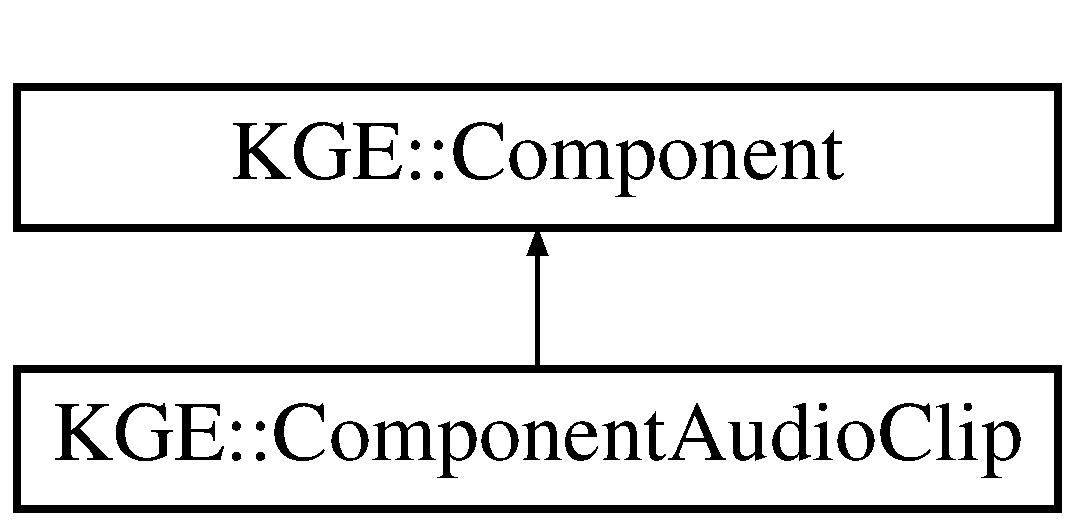
\includegraphics[height=2.000000cm]{class_k_g_e_1_1_component_audio_clip}
\end{center}
\end{figure}
\subsection*{Additional Inherited Members}


The documentation for this class was generated from the following file\-:\begin{DoxyCompactItemize}
\item 
C\-:/\-Users/\-Vit/\-Documents/\-Git\-Hub/\-K\-G\-E/\-K\-G\-E/\-Core/\-Audio/Component\-Audio\-Clip.\-hpp\end{DoxyCompactItemize}

\hypertarget{class_k_g_e_1_1_component_button}{\section{K\-G\-E\-:\-:Component\-Button Class Reference}
\label{class_k_g_e_1_1_component_button}\index{K\-G\-E\-::\-Component\-Button@{K\-G\-E\-::\-Component\-Button}}
}
Inheritance diagram for K\-G\-E\-:\-:Component\-Button\-:\begin{figure}[H]
\begin{center}
\leavevmode
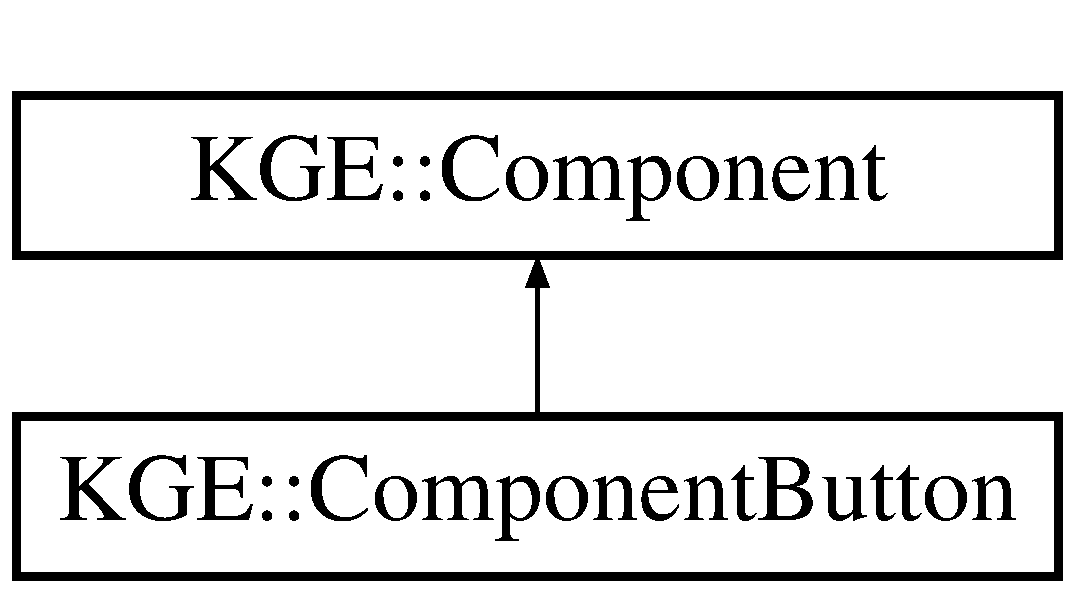
\includegraphics[height=2.000000cm]{class_k_g_e_1_1_component_button}
\end{center}
\end{figure}
\subsection*{Additional Inherited Members}


The documentation for this class was generated from the following file\-:\begin{DoxyCompactItemize}
\item 
C\-:/\-Users/\-Vit/\-Documents/\-Git\-Hub/\-K\-G\-E/\-K\-G\-E/\-Core/\-Interface/Component\-Button.\-hpp\end{DoxyCompactItemize}

\hypertarget{class_k_g_e_1_1_component_camera_layer}{\section{K\-G\-E\-:\-:Component\-Camera\-Layer Class Reference}
\label{class_k_g_e_1_1_component_camera_layer}\index{K\-G\-E\-::\-Component\-Camera\-Layer@{K\-G\-E\-::\-Component\-Camera\-Layer}}
}
Inheritance diagram for K\-G\-E\-:\-:Component\-Camera\-Layer\-:\begin{figure}[H]
\begin{center}
\leavevmode
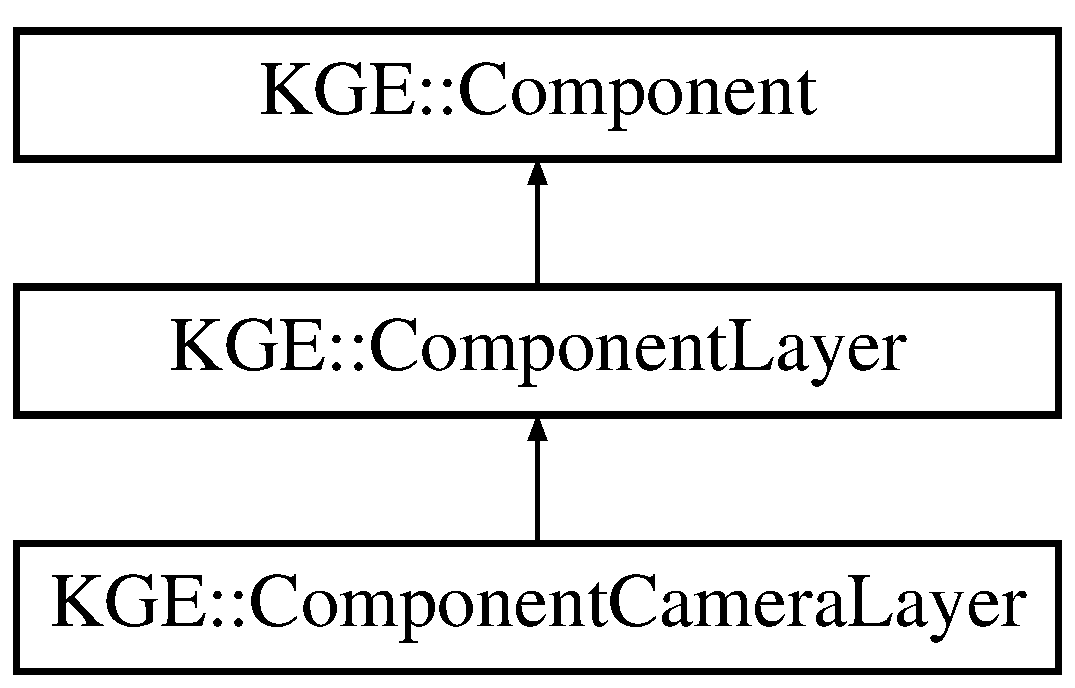
\includegraphics[height=3.000000cm]{class_k_g_e_1_1_component_camera_layer}
\end{center}
\end{figure}
\subsection*{Additional Inherited Members}


The documentation for this class was generated from the following file\-:\begin{DoxyCompactItemize}
\item 
C\-:/\-Users/\-Vit/\-Documents/\-Git\-Hub/\-K\-G\-E/\-K\-G\-E/\-Core/\-Components/\-Basic/Component\-Camera\-Layer.\-hpp\end{DoxyCompactItemize}

\hypertarget{class_k_g_e_1_1_component_collection}{\section{K\-G\-E\-:\-:Component\-Collection Class Reference}
\label{class_k_g_e_1_1_component_collection}\index{K\-G\-E\-::\-Component\-Collection@{K\-G\-E\-::\-Component\-Collection}}
}
Inheritance diagram for K\-G\-E\-:\-:Component\-Collection\-:\begin{figure}[H]
\begin{center}
\leavevmode
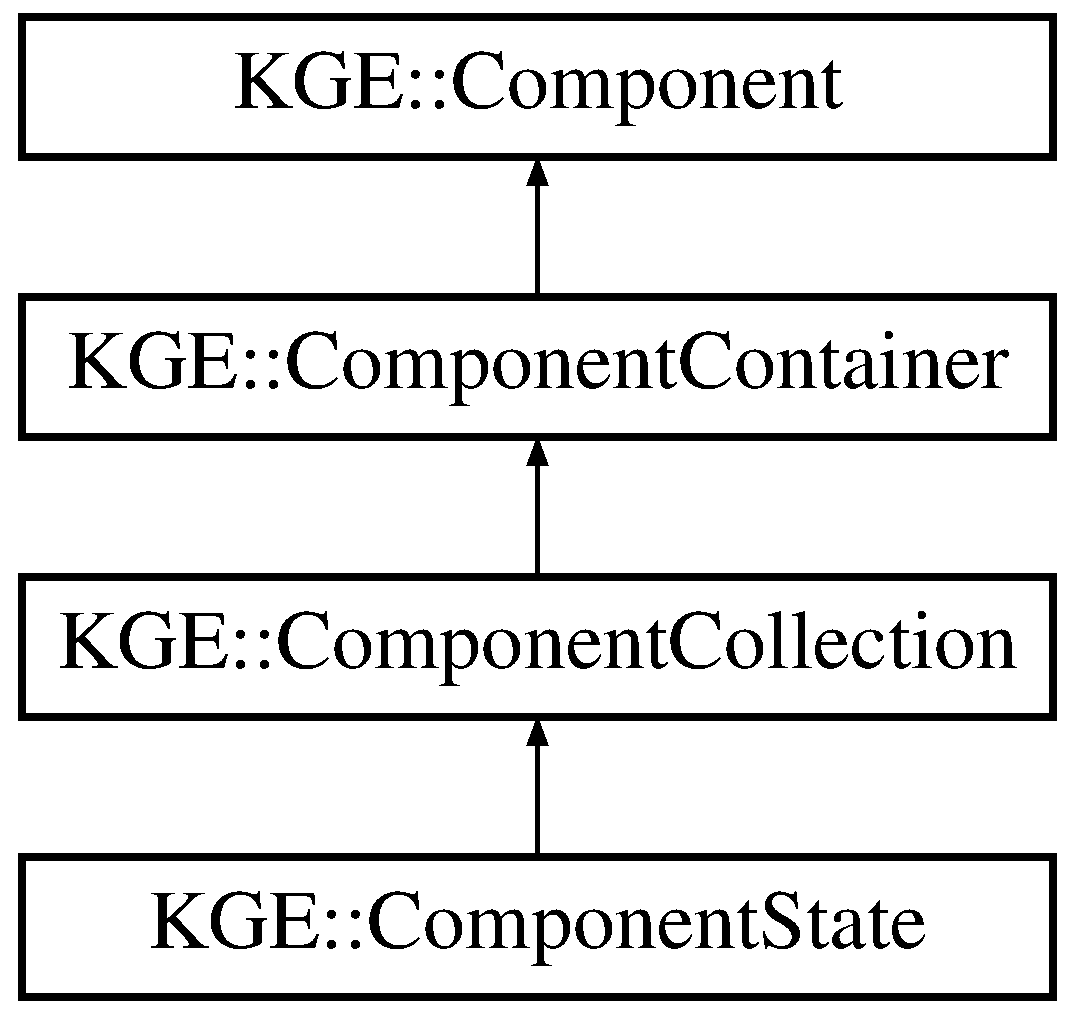
\includegraphics[height=4.000000cm]{class_k_g_e_1_1_component_collection}
\end{center}
\end{figure}
\subsection*{Additional Inherited Members}


The documentation for this class was generated from the following file\-:\begin{DoxyCompactItemize}
\item 
C\-:/\-Users/\-Vit/\-Documents/\-Git\-Hub/\-K\-G\-E/\-K\-G\-E/\-Core/\-Components/Component\-Collection.\-hpp\end{DoxyCompactItemize}

\hypertarget{class_k_g_e_1_1_component_composite}{\section{K\-G\-E\-:\-:Component\-Composite Class Reference}
\label{class_k_g_e_1_1_component_composite}\index{K\-G\-E\-::\-Component\-Composite@{K\-G\-E\-::\-Component\-Composite}}
}
Inheritance diagram for K\-G\-E\-:\-:Component\-Composite\-:\begin{figure}[H]
\begin{center}
\leavevmode
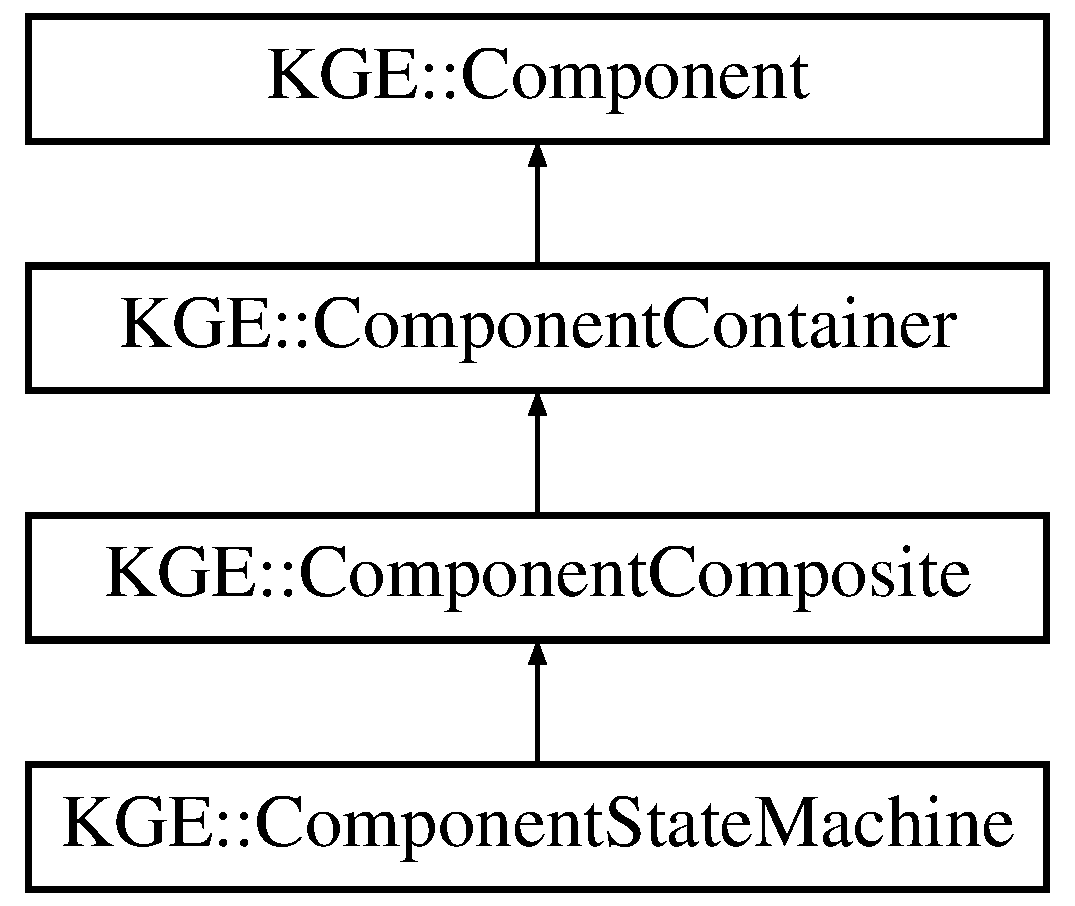
\includegraphics[height=4.000000cm]{class_k_g_e_1_1_component_composite}
\end{center}
\end{figure}
\subsection*{Additional Inherited Members}


The documentation for this class was generated from the following files\-:\begin{DoxyCompactItemize}
\item 
C\-:/\-Users/\-Vit/\-Documents/\-Git\-Hub/\-K\-G\-E/\-K\-G\-E/\-Core/\-Components/Component\-Composite.\-hpp\item 
C\-:/\-Users/\-Vit/\-Documents/\-Git\-Hub/\-K\-G\-E/\-K\-G\-E/\-Core/\-Components/Component\-Composite.\-cpp\end{DoxyCompactItemize}

\hypertarget{class_k_g_e_1_1_component_container}{\section{K\-G\-E\-:\-:Component\-Container Class Reference}
\label{class_k_g_e_1_1_component_container}\index{K\-G\-E\-::\-Component\-Container@{K\-G\-E\-::\-Component\-Container}}
}
Inheritance diagram for K\-G\-E\-:\-:Component\-Container\-:\begin{figure}[H]
\begin{center}
\leavevmode
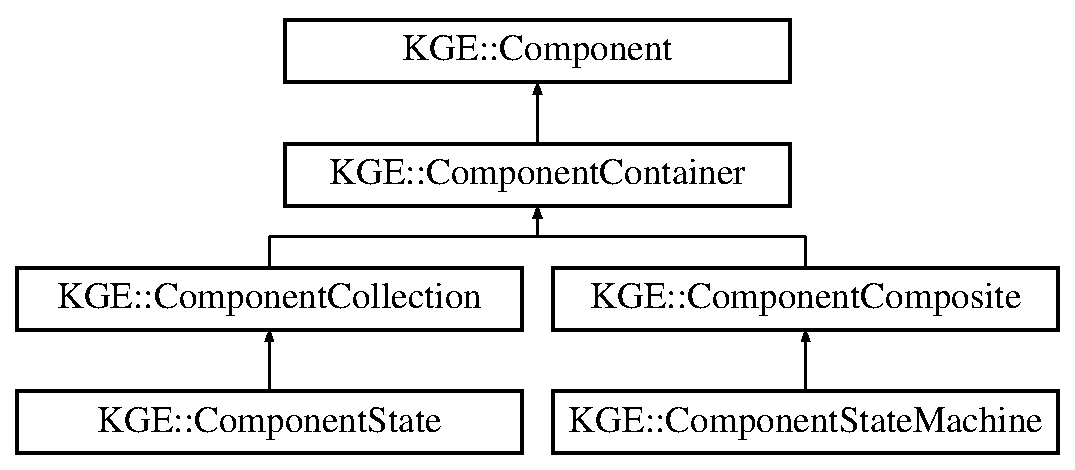
\includegraphics[height=4.000000cm]{class_k_g_e_1_1_component_container}
\end{center}
\end{figure}
\subsection*{Public Member Functions}
\begin{DoxyCompactItemize}
\item 
\hypertarget{class_k_g_e_1_1_component_container_ad12b900ef00af93b7c8560ec3195762e}{{\bfseries Component\-Container} (\hyperlink{class_k_g_e_1_1_t_u_i_d}{T\-U\-I\-D}$<$ \hyperlink{class_k_g_e_1_1_component}{Component} $>$\-::Cached\-Reference x\-Parent)}\label{class_k_g_e_1_1_component_container_ad12b900ef00af93b7c8560ec3195762e}

\item 
\hypertarget{class_k_g_e_1_1_component_container_aee612c9e180ebe71e6b46f8a8baf778d}{{\bfseries Component\-Container} (xml\-\_\-node$<$ char $>$ \&x\-Node, \hyperlink{class_k_g_e_1_1_t_u_i_d}{T\-U\-I\-D}$<$ \hyperlink{class_k_g_e_1_1_component}{Component} $>$\-::Cached\-Reference x\-Parent)}\label{class_k_g_e_1_1_component_container_aee612c9e180ebe71e6b46f8a8baf778d}

\item 
\hypertarget{class_k_g_e_1_1_component_container_af830c7777cc2bb5ee14453a53d34789e}{virtual void {\bfseries On\-Activate} (eventparams\-\_\-t \&x\-Event\-Parameters)}\label{class_k_g_e_1_1_component_container_af830c7777cc2bb5ee14453a53d34789e}

\item 
\hypertarget{class_k_g_e_1_1_component_container_a763825608230c978d6df1662793cb547}{virtual void {\bfseries On\-Deactivate} (eventparams\-\_\-t \&x\-Event\-Parameters)}\label{class_k_g_e_1_1_component_container_a763825608230c978d6df1662793cb547}

\item 
\hypertarget{class_k_g_e_1_1_component_container_ac8dd90ad88772cd83f0c2054cc65d918}{virtual void {\bfseries On\-Destroy} (eventparams\-\_\-t \&x\-Event\-Parameters)}\label{class_k_g_e_1_1_component_container_ac8dd90ad88772cd83f0c2054cc65d918}

\end{DoxyCompactItemize}
\subsection*{Protected Member Functions}
\begin{DoxyCompactItemize}
\item 
\hypertarget{class_k_g_e_1_1_component_container_a9126f38630214eb22f670d1f07f78e1c}{void {\bfseries Populate\-Component} (xml\-\_\-node$<$ char $>$ \&x\-Component\-Node)}\label{class_k_g_e_1_1_component_container_a9126f38630214eb22f670d1f07f78e1c}

\end{DoxyCompactItemize}
\subsection*{Protected Attributes}
\begin{DoxyCompactItemize}
\item 
\hypertarget{class_k_g_e_1_1_component_container_a745972f0622830dc7380e5dd91016071}{componentcontainer\-\_\-t {\bfseries m\-\_\-x\-Components}}\label{class_k_g_e_1_1_component_container_a745972f0622830dc7380e5dd91016071}

\end{DoxyCompactItemize}
\subsection*{Additional Inherited Members}


The documentation for this class was generated from the following files\-:\begin{DoxyCompactItemize}
\item 
C\-:/\-Users/\-Vit/\-Documents/\-Git\-Hub/\-K\-G\-E/\-K\-G\-E/\-Core/\-Components/Component.\-hpp\item 
C\-:/\-Users/\-Vit/\-Documents/\-Git\-Hub/\-K\-G\-E/\-K\-G\-E/\-Core/\-Components/Component.\-cpp\end{DoxyCompactItemize}

\hypertarget{class_k_g_e_1_1_component_layer}{\section{K\-G\-E\-:\-:Component\-Layer Class Reference}
\label{class_k_g_e_1_1_component_layer}\index{K\-G\-E\-::\-Component\-Layer@{K\-G\-E\-::\-Component\-Layer}}
}
Inheritance diagram for K\-G\-E\-:\-:Component\-Layer\-:\begin{figure}[H]
\begin{center}
\leavevmode
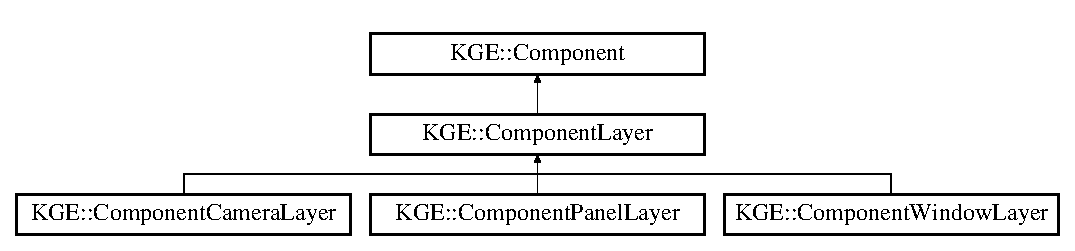
\includegraphics[height=2.931937cm]{class_k_g_e_1_1_component_layer}
\end{center}
\end{figure}
\subsection*{Protected Attributes}
\begin{DoxyCompactItemize}
\item 
\hypertarget{class_k_g_e_1_1_component_layer_a8e4c60d1b64f97420621fe5e108683d0}{componentcontainer\-\_\-t {\bfseries m\-\_\-x\-Handle\-Input\-List}}\label{class_k_g_e_1_1_component_layer_a8e4c60d1b64f97420621fe5e108683d0}

\item 
\hypertarget{class_k_g_e_1_1_component_layer_aa2d8c0ddbd70e762e2168438237c58b1}{componentcontainer\-\_\-t {\bfseries m\-\_\-x\-Render\-List}}\label{class_k_g_e_1_1_component_layer_aa2d8c0ddbd70e762e2168438237c58b1}

\end{DoxyCompactItemize}
\subsection*{Additional Inherited Members}


The documentation for this class was generated from the following files\-:\begin{DoxyCompactItemize}
\item 
C\-:/\-Users/\-Vit/\-Documents/\-Git\-Hub/\-K\-G\-E/\-K\-G\-E/\-Core/\-Components/\-Basic/Component\-Layer.\-hpp\item 
C\-:/\-Users/\-Vit/\-Documents/\-Git\-Hub/\-K\-G\-E/\-K\-G\-E/\-Core/\-Components/\-Basic/Component\-Layer.\-cpp\end{DoxyCompactItemize}

\hypertarget{class_k_g_e_1_1_component_music}{\section{K\-G\-E\-:\-:Component\-Music Class Reference}
\label{class_k_g_e_1_1_component_music}\index{K\-G\-E\-::\-Component\-Music@{K\-G\-E\-::\-Component\-Music}}
}
Inheritance diagram for K\-G\-E\-:\-:Component\-Music\-:\begin{figure}[H]
\begin{center}
\leavevmode
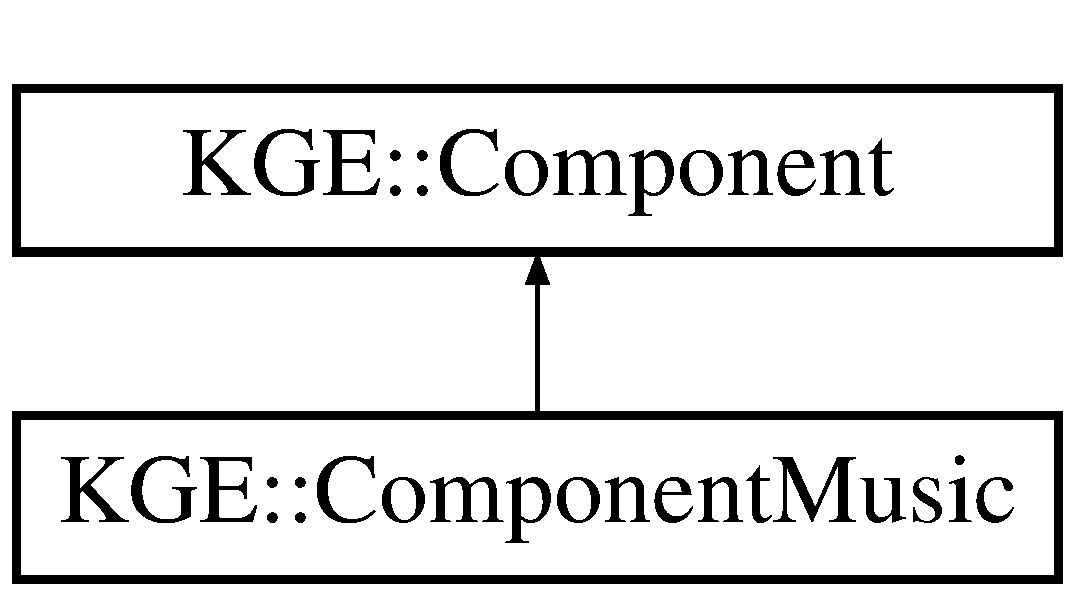
\includegraphics[height=2.000000cm]{class_k_g_e_1_1_component_music}
\end{center}
\end{figure}
\subsection*{Additional Inherited Members}


The documentation for this class was generated from the following file\-:\begin{DoxyCompactItemize}
\item 
C\-:/\-Users/\-Vit/\-Documents/\-Git\-Hub/\-K\-G\-E/\-K\-G\-E/\-Core/\-Audio/Component\-Music.\-hpp\end{DoxyCompactItemize}

\hypertarget{class_k_g_e_1_1_component_panel_layer}{\section{K\-G\-E\-:\-:Component\-Panel\-Layer Class Reference}
\label{class_k_g_e_1_1_component_panel_layer}\index{K\-G\-E\-::\-Component\-Panel\-Layer@{K\-G\-E\-::\-Component\-Panel\-Layer}}
}
Inheritance diagram for K\-G\-E\-:\-:Component\-Panel\-Layer\-:\begin{figure}[H]
\begin{center}
\leavevmode
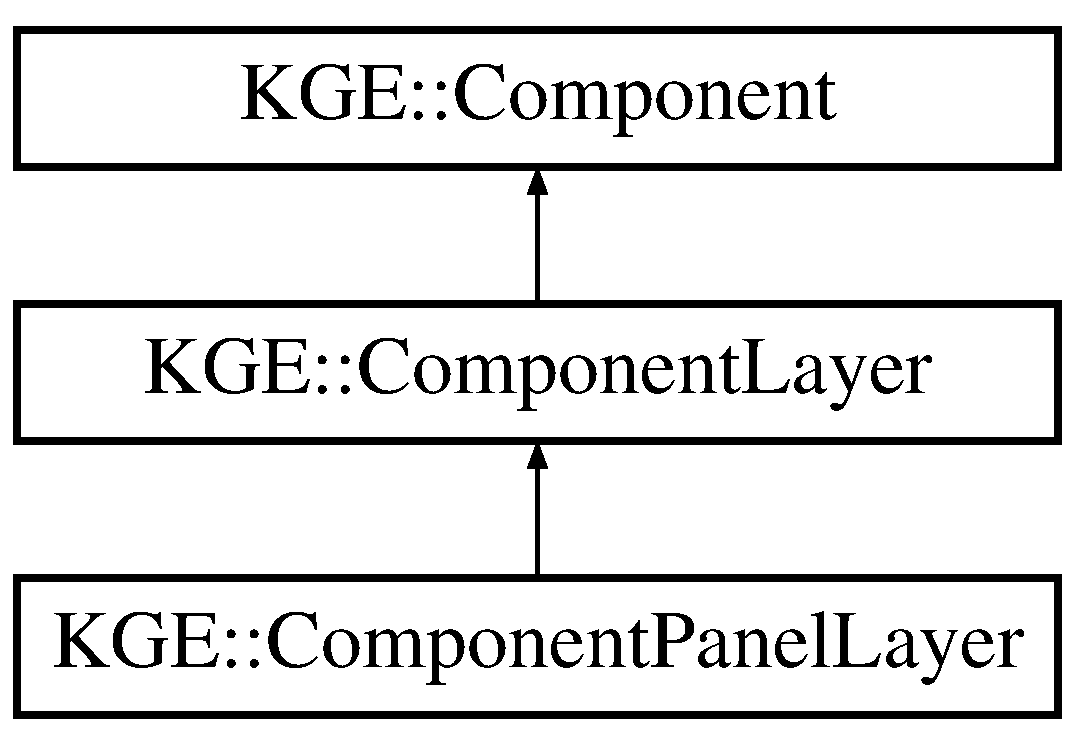
\includegraphics[height=3.000000cm]{class_k_g_e_1_1_component_panel_layer}
\end{center}
\end{figure}
\subsection*{Additional Inherited Members}


The documentation for this class was generated from the following file\-:\begin{DoxyCompactItemize}
\item 
C\-:/\-Users/\-Vit/\-Documents/\-Git\-Hub/\-K\-G\-E/\-K\-G\-E/\-Core/\-Components/\-Basic/Component\-Panel\-Layer.\-hpp\end{DoxyCompactItemize}

\hypertarget{class_k_g_e_1_1_component_sprite}{\section{K\-G\-E\-:\-:Component\-Sprite Class Reference}
\label{class_k_g_e_1_1_component_sprite}\index{K\-G\-E\-::\-Component\-Sprite@{K\-G\-E\-::\-Component\-Sprite}}
}
Inheritance diagram for K\-G\-E\-:\-:Component\-Sprite\-:\begin{figure}[H]
\begin{center}
\leavevmode
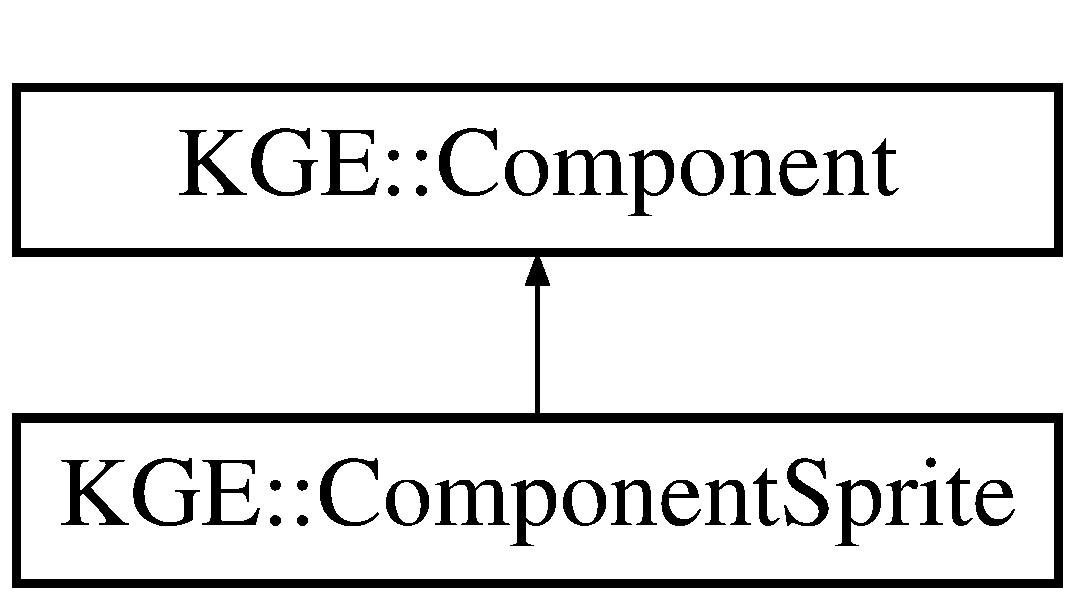
\includegraphics[height=2.000000cm]{class_k_g_e_1_1_component_sprite}
\end{center}
\end{figure}
\subsection*{Additional Inherited Members}


The documentation for this class was generated from the following file\-:\begin{DoxyCompactItemize}
\item 
C\-:/\-Users/\-Vit/\-Documents/\-Git\-Hub/\-K\-G\-E/\-K\-G\-E/\-Core/\-Graphics/Component\-Sprite.\-hpp\end{DoxyCompactItemize}

\hypertarget{class_k_g_e_1_1_component_state}{\section{K\-G\-E\-:\-:Component\-State Class Reference}
\label{class_k_g_e_1_1_component_state}\index{K\-G\-E\-::\-Component\-State@{K\-G\-E\-::\-Component\-State}}
}
Inheritance diagram for K\-G\-E\-:\-:Component\-State\-:\begin{figure}[H]
\begin{center}
\leavevmode
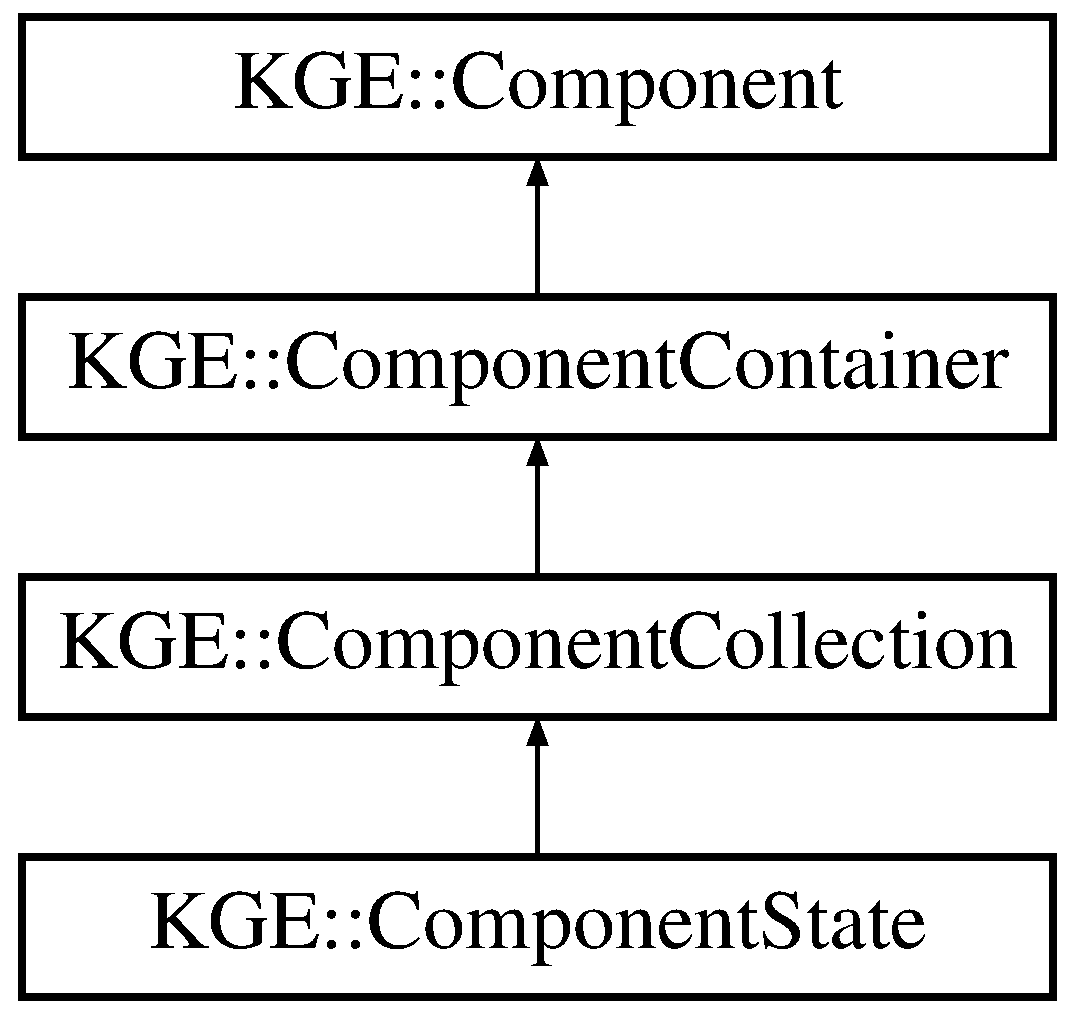
\includegraphics[height=4.000000cm]{class_k_g_e_1_1_component_state}
\end{center}
\end{figure}
\subsection*{Additional Inherited Members}


The documentation for this class was generated from the following file\-:\begin{DoxyCompactItemize}
\item 
C\-:/\-Users/\-Vit/\-Documents/\-Git\-Hub/\-K\-G\-E/\-K\-G\-E/\-Core/\-A\-I/Component\-State.\-hpp\end{DoxyCompactItemize}

\hypertarget{class_k_g_e_1_1_component_state_machine}{\section{K\-G\-E\-:\-:Component\-State\-Machine Class Reference}
\label{class_k_g_e_1_1_component_state_machine}\index{K\-G\-E\-::\-Component\-State\-Machine@{K\-G\-E\-::\-Component\-State\-Machine}}
}
Inheritance diagram for K\-G\-E\-:\-:Component\-State\-Machine\-:\begin{figure}[H]
\begin{center}
\leavevmode
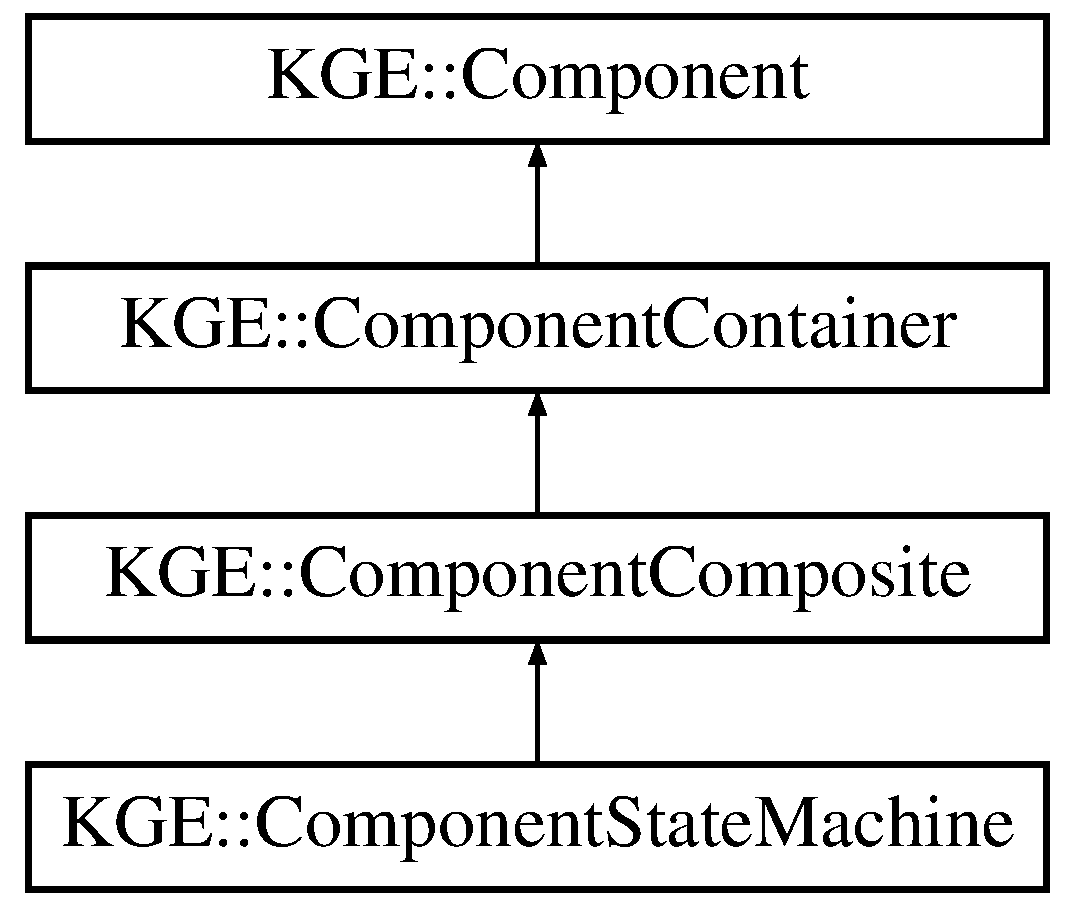
\includegraphics[height=4.000000cm]{class_k_g_e_1_1_component_state_machine}
\end{center}
\end{figure}
\subsection*{Public Member Functions}
\begin{DoxyCompactItemize}
\item 
\hypertarget{class_k_g_e_1_1_component_state_machine_a746c723bc378d677011aa4b53f88bcbe}{{\bfseries Component\-State\-Machine} (\hyperlink{class_k_g_e_1_1_t_u_i_d}{T\-U\-I\-D}$<$ \hyperlink{class_k_g_e_1_1_component}{Component} $>$\-::Cached\-Reference x\-Parent)}\label{class_k_g_e_1_1_component_state_machine_a746c723bc378d677011aa4b53f88bcbe}

\item 
\hypertarget{class_k_g_e_1_1_component_state_machine_a904e7640f0987d5efee2555976df811d}{{\bfseries Component\-State\-Machine} (xml\-\_\-node$<$ char $>$ \&x\-Node, \hyperlink{class_k_g_e_1_1_t_u_i_d}{T\-U\-I\-D}$<$ \hyperlink{class_k_g_e_1_1_component}{Component} $>$\-::Cached\-Reference x\-Parent)}\label{class_k_g_e_1_1_component_state_machine_a904e7640f0987d5efee2555976df811d}

\item 
\hypertarget{class_k_g_e_1_1_component_state_machine_a65dbfbf05f45eb56cfe9a2f347f7c7c4}{virtual void {\bfseries On\-Activate} (eventparams\-\_\-t \&x\-Event\-Parameters)}\label{class_k_g_e_1_1_component_state_machine_a65dbfbf05f45eb56cfe9a2f347f7c7c4}

\item 
\hypertarget{class_k_g_e_1_1_component_state_machine_a93ec82209352e3f96d010bc457c8f22d}{virtual void {\bfseries On\-Deactivate} (eventparams\-\_\-t \&x\-Event\-Parameters)}\label{class_k_g_e_1_1_component_state_machine_a93ec82209352e3f96d010bc457c8f22d}

\item 
\hypertarget{class_k_g_e_1_1_component_state_machine_a98d710868fd9ec049a4852be56e6c35c}{virtual void {\bfseries On\-Destroy} (eventparams\-\_\-t \&x\-Event\-Parameters)}\label{class_k_g_e_1_1_component_state_machine_a98d710868fd9ec049a4852be56e6c35c}

\item 
\hypertarget{class_k_g_e_1_1_component_state_machine_ad52c88d8693f44464609e365787dd22a}{virtual void {\bfseries On\-Change\-State} (eventparams\-\_\-t \&x\-Event\-Parameters)}\label{class_k_g_e_1_1_component_state_machine_ad52c88d8693f44464609e365787dd22a}

\item 
\hypertarget{class_k_g_e_1_1_component_state_machine_a0f5e40be63810f0566219a725f725f5b}{virtual void {\bfseries Set\-State} (const \hyperlink{class_k_g_e_1_1_hash}{Hash} \&x\-State\-Hash)}\label{class_k_g_e_1_1_component_state_machine_a0f5e40be63810f0566219a725f725f5b}

\end{DoxyCompactItemize}
\subsection*{Protected Member Functions}
\begin{DoxyCompactItemize}
\item 
\hypertarget{class_k_g_e_1_1_component_state_machine_a5a0193964976a9cdbf7df765bb77c444}{void {\bfseries Register\-Events} ()}\label{class_k_g_e_1_1_component_state_machine_a5a0193964976a9cdbf7df765bb77c444}

\item 
\hypertarget{class_k_g_e_1_1_component_state_machine_a4b4662d44a1b659ebf6cf9504f82c4b9}{virtual void {\bfseries Populate\-Initial\-State} (xml\-\_\-attribute$<$ char $>$ \&x\-Initial\-State)}\label{class_k_g_e_1_1_component_state_machine_a4b4662d44a1b659ebf6cf9504f82c4b9}

\item 
\hypertarget{class_k_g_e_1_1_component_state_machine_a518cd4b1c2c8af852109f2ffb7e9b3ae}{virtual void {\bfseries Populate\-State} (xml\-\_\-node$<$ char $>$ \&x\-State)}\label{class_k_g_e_1_1_component_state_machine_a518cd4b1c2c8af852109f2ffb7e9b3ae}

\end{DoxyCompactItemize}
\subsection*{Protected Attributes}
\begin{DoxyCompactItemize}
\item 
\hypertarget{class_k_g_e_1_1_component_state_machine_a8c59f416a93dc7eec37fb6cd0b90d488}{\hyperlink{class_k_g_e_1_1_hash}{Hash} {\bfseries m\-\_\-x\-Initial\-State}}\label{class_k_g_e_1_1_component_state_machine_a8c59f416a93dc7eec37fb6cd0b90d488}

\item 
\hypertarget{class_k_g_e_1_1_component_state_machine_a37c5962df358e40bd8c0807c0dd143ec}{\hyperlink{class_k_g_e_1_1_component_state}{Component\-State} $\ast$ {\bfseries m\-\_\-px\-Current\-State}}\label{class_k_g_e_1_1_component_state_machine_a37c5962df358e40bd8c0807c0dd143ec}

\item 
\hypertarget{class_k_g_e_1_1_component_state_machine_a6a9b3302a8b0b76c7bf6292683dd3b78}{unordered\-\_\-map$<$ \hyperlink{class_k_g_e_1_1_hash}{Hash}, xml\-\_\-node\\*
$<$ char $>$ $\ast$, \hyperlink{struct_k_g_e_1_1_hash_1_1_hasher}{Hash\-::\-Hasher} $>$ {\bfseries m\-\_\-x\-States}}\label{class_k_g_e_1_1_component_state_machine_a6a9b3302a8b0b76c7bf6292683dd3b78}

\end{DoxyCompactItemize}
\subsection*{Additional Inherited Members}


The documentation for this class was generated from the following files\-:\begin{DoxyCompactItemize}
\item 
C\-:/\-Users/\-Vit/\-Documents/\-Git\-Hub/\-K\-G\-E/\-K\-G\-E/\-Core/\-A\-I/Component\-State\-Machine.\-hpp\item 
C\-:/\-Users/\-Vit/\-Documents/\-Git\-Hub/\-K\-G\-E/\-K\-G\-E/\-Core/\-A\-I/Component\-State\-Machine.\-cpp\end{DoxyCompactItemize}

\hypertarget{class_k_g_e_1_1_component_updater}{\section{K\-G\-E\-:\-:Component\-Updater Class Reference}
\label{class_k_g_e_1_1_component_updater}\index{K\-G\-E\-::\-Component\-Updater@{K\-G\-E\-::\-Component\-Updater}}
}
Inheritance diagram for K\-G\-E\-:\-:Component\-Updater\-:\begin{figure}[H]
\begin{center}
\leavevmode
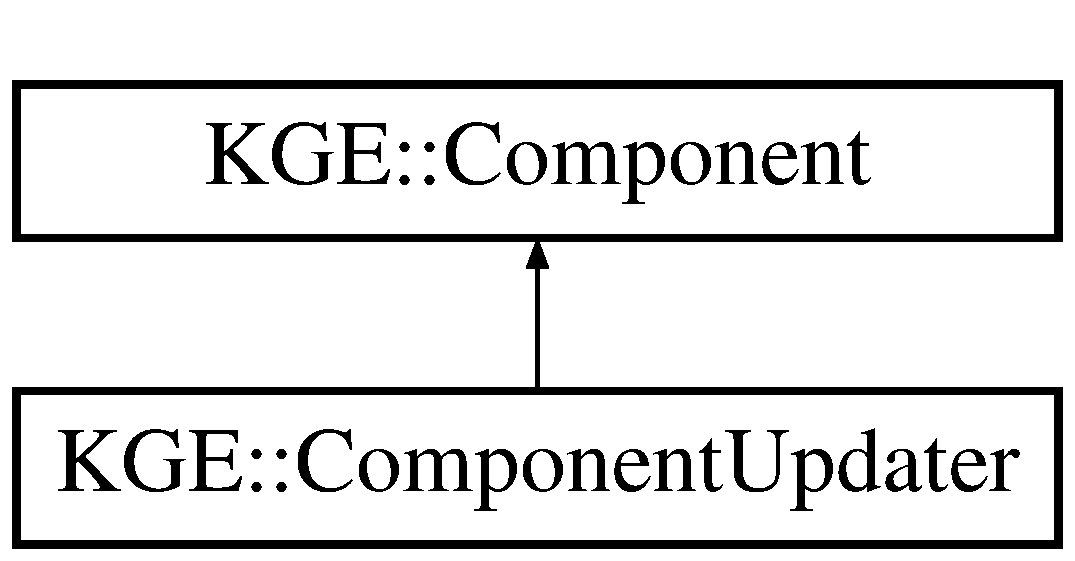
\includegraphics[height=2.000000cm]{class_k_g_e_1_1_component_updater}
\end{center}
\end{figure}
\subsection*{Protected Attributes}
\begin{DoxyCompactItemize}
\item 
\hypertarget{class_k_g_e_1_1_component_updater_aa2d8cfa86df1a05b5f7eb107d136a3b7}{componentcontainer\-\_\-t {\bfseries m\-\_\-x\-Update\-List}}\label{class_k_g_e_1_1_component_updater_aa2d8cfa86df1a05b5f7eb107d136a3b7}

\end{DoxyCompactItemize}
\subsection*{Static Protected Attributes}
\begin{DoxyCompactItemize}
\item 
\hypertarget{class_k_g_e_1_1_component_updater_a9aebe649bdac78f73812610046a4aa86}{static unordered\-\_\-set\\*
$<$ \hyperlink{class_k_g_e_1_1_component_updater}{Component\-Updater} $\ast$, Hasher $>$ {\bfseries s\-\_\-x\-All\-Updaters}}\label{class_k_g_e_1_1_component_updater_a9aebe649bdac78f73812610046a4aa86}

\end{DoxyCompactItemize}
\subsection*{Additional Inherited Members}


The documentation for this class was generated from the following files\-:\begin{DoxyCompactItemize}
\item 
C\-:/\-Users/\-Vit/\-Documents/\-Git\-Hub/\-K\-G\-E/\-K\-G\-E/\-Core/\-Components/\-Basic/Component\-Updater.\-hpp\item 
C\-:/\-Users/\-Vit/\-Documents/\-Git\-Hub/\-K\-G\-E/\-K\-G\-E/\-Core/\-Components/\-Basic/Component\-Updater.\-cpp\end{DoxyCompactItemize}

\hypertarget{class_k_g_e_1_1_component_window_layer}{\section{K\-G\-E\-:\-:Component\-Window\-Layer Class Reference}
\label{class_k_g_e_1_1_component_window_layer}\index{K\-G\-E\-::\-Component\-Window\-Layer@{K\-G\-E\-::\-Component\-Window\-Layer}}
}
Inheritance diagram for K\-G\-E\-:\-:Component\-Window\-Layer\-:\begin{figure}[H]
\begin{center}
\leavevmode
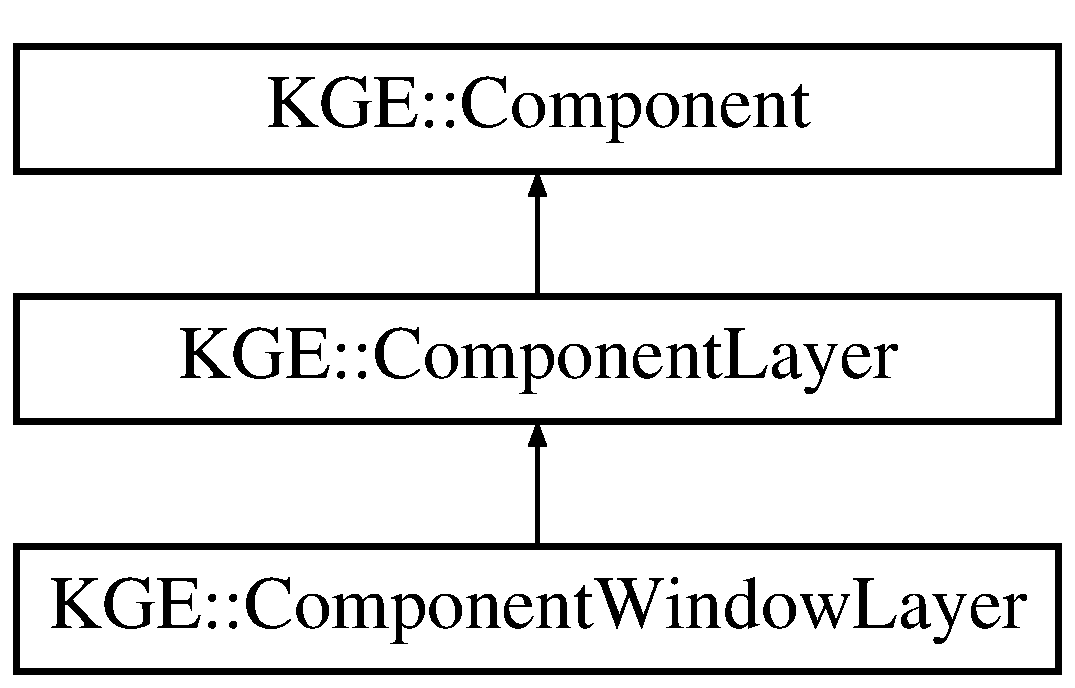
\includegraphics[height=3.000000cm]{class_k_g_e_1_1_component_window_layer}
\end{center}
\end{figure}
\subsection*{Classes}
\begin{DoxyCompactItemize}
\item 
struct \hyperlink{struct_k_g_e_1_1_component_window_layer_1_1_hasher}{Hasher}
\end{DoxyCompactItemize}
\subsection*{Public Member Functions}
\begin{DoxyCompactItemize}
\item 
\hypertarget{class_k_g_e_1_1_component_window_layer_adff3a5c837939b6834886eaddd61c8a0}{{\bfseries Component\-Window\-Layer} (\hyperlink{class_k_g_e_1_1_t_u_i_d}{T\-U\-I\-D}$<$ \hyperlink{class_k_g_e_1_1_component}{Component} $>$\-::Cached\-Reference x\-Parent)}\label{class_k_g_e_1_1_component_window_layer_adff3a5c837939b6834886eaddd61c8a0}

\item 
\hypertarget{class_k_g_e_1_1_component_window_layer_a913d14e032d315d2b9c692fed84bd060}{{\bfseries Component\-Window\-Layer} (xml\-\_\-node$<$ char $>$ \&x\-Node, \hyperlink{class_k_g_e_1_1_t_u_i_d}{T\-U\-I\-D}$<$ \hyperlink{class_k_g_e_1_1_component}{Component} $>$\-::Cached\-Reference x\-Parent)}\label{class_k_g_e_1_1_component_window_layer_a913d14e032d315d2b9c692fed84bd060}

\item 
\hypertarget{class_k_g_e_1_1_component_window_layer_ae112cb973520b10f89d56d33f8d21bcb}{virtual void {\bfseries Handle\-Input} ()}\label{class_k_g_e_1_1_component_window_layer_ae112cb973520b10f89d56d33f8d21bcb}

\item 
\hypertarget{class_k_g_e_1_1_component_window_layer_a5947ec5f47c149bf39a122befd470994}{virtual void {\bfseries Render} ()}\label{class_k_g_e_1_1_component_window_layer_a5947ec5f47c149bf39a122befd470994}

\item 
\hypertarget{class_k_g_e_1_1_component_window_layer_aa5d6ce2298b39010a7c158abc86e3037}{virtual void {\bfseries On\-Activate} (eventparams\-\_\-t \&x\-Event\-Parameters)}\label{class_k_g_e_1_1_component_window_layer_aa5d6ce2298b39010a7c158abc86e3037}

\item 
\hypertarget{class_k_g_e_1_1_component_window_layer_a9855c99a112704899a72e3d0976e02b0}{virtual void {\bfseries On\-Deactivate} (eventparams\-\_\-t \&x\-Event\-Parameters)}\label{class_k_g_e_1_1_component_window_layer_a9855c99a112704899a72e3d0976e02b0}

\end{DoxyCompactItemize}
\subsection*{Static Public Member Functions}
\begin{DoxyCompactItemize}
\item 
\hypertarget{class_k_g_e_1_1_component_window_layer_a30e4e97870e7e913dc1a5576b1601a4c}{static void {\bfseries Handle\-Input\-All} ()}\label{class_k_g_e_1_1_component_window_layer_a30e4e97870e7e913dc1a5576b1601a4c}

\item 
\hypertarget{class_k_g_e_1_1_component_window_layer_a17371ec97dd4ed985e50548b46f17b56}{static void {\bfseries Render\-All} ()}\label{class_k_g_e_1_1_component_window_layer_a17371ec97dd4ed985e50548b46f17b56}

\end{DoxyCompactItemize}
\subsection*{Protected Member Functions}
\begin{DoxyCompactItemize}
\item 
\hypertarget{class_k_g_e_1_1_component_window_layer_ac2c03f63683b526314d12e807a77f8d3}{virtual void {\bfseries Process\-Fullscreen} (xml\-\_\-attribute$<$ char $>$ \&x\-Name)}\label{class_k_g_e_1_1_component_window_layer_ac2c03f63683b526314d12e807a77f8d3}

\item 
\hypertarget{class_k_g_e_1_1_component_window_layer_af2247d2fff32c7b9c915e69ab1780e6e}{virtual void {\bfseries Process\-X\-Resolution} (xml\-\_\-attribute$<$ char $>$ \&x\-Name)}\label{class_k_g_e_1_1_component_window_layer_af2247d2fff32c7b9c915e69ab1780e6e}

\item 
\hypertarget{class_k_g_e_1_1_component_window_layer_a576eaf86f928b883a022121218458889}{virtual void {\bfseries Process\-Y\-Resolution} (xml\-\_\-attribute$<$ char $>$ \&x\-Name)}\label{class_k_g_e_1_1_component_window_layer_a576eaf86f928b883a022121218458889}

\end{DoxyCompactItemize}
\subsection*{Protected Attributes}
\begin{DoxyCompactItemize}
\item 
\hypertarget{class_k_g_e_1_1_component_window_layer_a6fbbd4e03bf3ffbe2190e3529665c6af}{sf\-::\-Render\-Window $\ast$ {\bfseries m\-\_\-px\-Window}}\label{class_k_g_e_1_1_component_window_layer_a6fbbd4e03bf3ffbe2190e3529665c6af}

\item 
\hypertarget{class_k_g_e_1_1_component_window_layer_a9ab9cfb60882471333b2bfb7f7065e69}{bool {\bfseries m\-\_\-b\-Fullscreen}}\label{class_k_g_e_1_1_component_window_layer_a9ab9cfb60882471333b2bfb7f7065e69}

\item 
\hypertarget{class_k_g_e_1_1_component_window_layer_ae9814c5fdc41c8020805af4dc0b8b6f9}{bool {\bfseries m\-\_\-b\-Native\-Resolution}}\label{class_k_g_e_1_1_component_window_layer_ae9814c5fdc41c8020805af4dc0b8b6f9}

\item 
\hypertarget{class_k_g_e_1_1_component_window_layer_aa90ae11ee4bb4a9e6b03557d6e78414c}{int {\bfseries m\-\_\-i\-X\-Resolution}}\label{class_k_g_e_1_1_component_window_layer_aa90ae11ee4bb4a9e6b03557d6e78414c}

\item 
\hypertarget{class_k_g_e_1_1_component_window_layer_a2612b10d8401d27e43bf429abb7d51f9}{int {\bfseries m\-\_\-i\-Y\-Resolution}}\label{class_k_g_e_1_1_component_window_layer_a2612b10d8401d27e43bf429abb7d51f9}

\end{DoxyCompactItemize}
\subsection*{Static Protected Attributes}
\begin{DoxyCompactItemize}
\item 
\hypertarget{class_k_g_e_1_1_component_window_layer_a03c90d11942ce14f555bae76356a560b}{static unordered\-\_\-set\\*
$<$ \hyperlink{class_k_g_e_1_1_component_window_layer}{Component\-Window\-Layer} \\*
$\ast$, \hyperlink{struct_k_g_e_1_1_component_window_layer_1_1_hasher}{Hasher} $>$ {\bfseries s\-\_\-x\-All\-Windows}}\label{class_k_g_e_1_1_component_window_layer_a03c90d11942ce14f555bae76356a560b}

\end{DoxyCompactItemize}
\subsection*{Additional Inherited Members}


The documentation for this class was generated from the following files\-:\begin{DoxyCompactItemize}
\item 
C\-:/\-Users/\-Vit/\-Documents/\-Git\-Hub/\-K\-G\-E/\-K\-G\-E/\-Core/\-Components/\-Basic/Component\-Window\-Layer.\-hpp\item 
C\-:/\-Users/\-Vit/\-Documents/\-Git\-Hub/\-K\-G\-E/\-K\-G\-E/\-Core/\-Components/\-Basic/Component\-Window\-Layer.\-cpp\end{DoxyCompactItemize}

\hypertarget{class_k_g_e_1_1_create_functor}{\section{K\-G\-E\-:\-:Create\-Functor$<$ root\-\_\-t, this\-\_\-t $>$ Class Template Reference}
\label{class_k_g_e_1_1_create_functor}\index{K\-G\-E\-::\-Create\-Functor$<$ root\-\_\-t, this\-\_\-t $>$@{K\-G\-E\-::\-Create\-Functor$<$ root\-\_\-t, this\-\_\-t $>$}}
}
Inheritance diagram for K\-G\-E\-:\-:Create\-Functor$<$ root\-\_\-t, this\-\_\-t $>$\-:\begin{figure}[H]
\begin{center}
\leavevmode
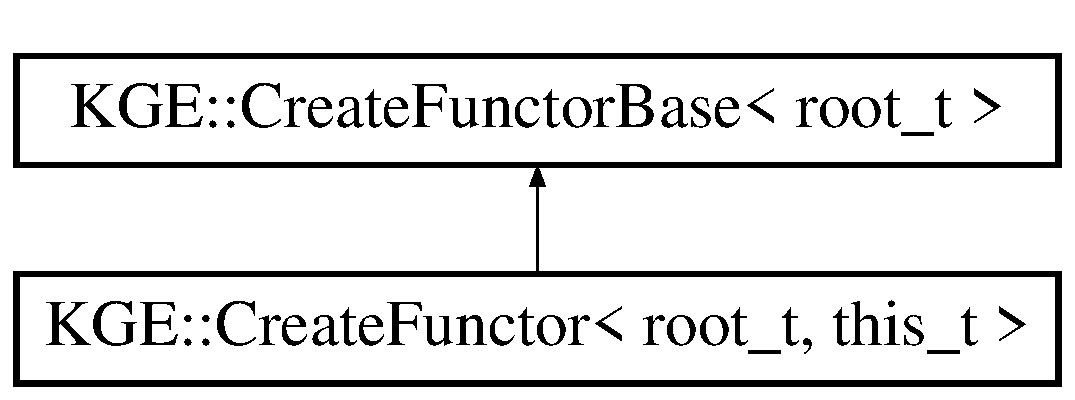
\includegraphics[height=2.000000cm]{class_k_g_e_1_1_create_functor}
\end{center}
\end{figure}
\subsection*{Public Member Functions}
\begin{DoxyCompactItemize}
\item 
\hypertarget{class_k_g_e_1_1_create_functor_a488fd93790fe3db78de1d435e272024e}{virtual root\-\_\-t $\ast$ {\bfseries operator()} ()}\label{class_k_g_e_1_1_create_functor_a488fd93790fe3db78de1d435e272024e}

\end{DoxyCompactItemize}


The documentation for this class was generated from the following file\-:\begin{DoxyCompactItemize}
\item 
C\-:/\-Users/\-Vit/\-Documents/\-Git\-Hub/\-K\-G\-E/\-K\-G\-E/\-Core/\-Class\-Capabilities/Class\-Factory.\-hpp\end{DoxyCompactItemize}

\hypertarget{class_k_g_e_1_1_create_functor1_arg}{\section{K\-G\-E\-:\-:Create\-Functor1\-Arg$<$ root\-\_\-t, this\-\_\-t, arg0\-\_\-t $>$ Class Template Reference}
\label{class_k_g_e_1_1_create_functor1_arg}\index{K\-G\-E\-::\-Create\-Functor1\-Arg$<$ root\-\_\-t, this\-\_\-t, arg0\-\_\-t $>$@{K\-G\-E\-::\-Create\-Functor1\-Arg$<$ root\-\_\-t, this\-\_\-t, arg0\-\_\-t $>$}}
}
Inheritance diagram for K\-G\-E\-:\-:Create\-Functor1\-Arg$<$ root\-\_\-t, this\-\_\-t, arg0\-\_\-t $>$\-:\begin{figure}[H]
\begin{center}
\leavevmode
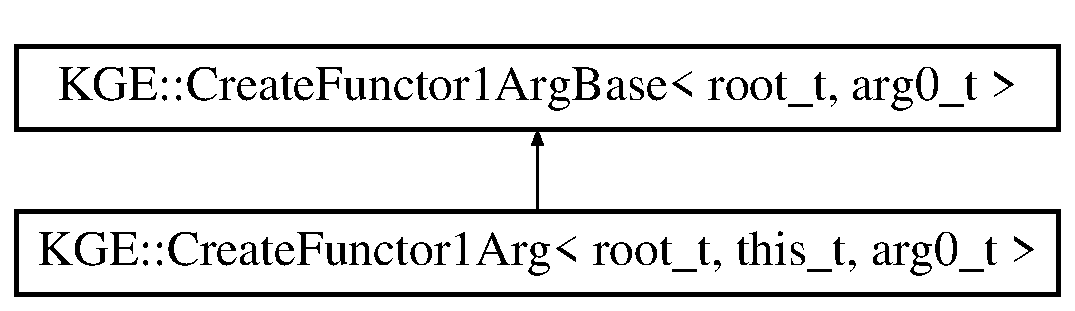
\includegraphics[height=2.000000cm]{class_k_g_e_1_1_create_functor1_arg}
\end{center}
\end{figure}
\subsection*{Public Member Functions}
\begin{DoxyCompactItemize}
\item 
\hypertarget{class_k_g_e_1_1_create_functor1_arg_aabc7a3edb3f9d67cdeba51146686a4de}{virtual root\-\_\-t $\ast$ {\bfseries operator()} (arg0\-\_\-t x\-Arg0)}\label{class_k_g_e_1_1_create_functor1_arg_aabc7a3edb3f9d67cdeba51146686a4de}

\end{DoxyCompactItemize}


The documentation for this class was generated from the following file\-:\begin{DoxyCompactItemize}
\item 
C\-:/\-Users/\-Vit/\-Documents/\-Git\-Hub/\-K\-G\-E/\-K\-G\-E/\-Core/\-Class\-Capabilities/Class\-Factory.\-hpp\end{DoxyCompactItemize}

\hypertarget{class_k_g_e_1_1_create_functor1_arg_base}{\section{K\-G\-E\-:\-:Create\-Functor1\-Arg\-Base$<$ root\-\_\-t, arg0\-\_\-t $>$ Class Template Reference}
\label{class_k_g_e_1_1_create_functor1_arg_base}\index{K\-G\-E\-::\-Create\-Functor1\-Arg\-Base$<$ root\-\_\-t, arg0\-\_\-t $>$@{K\-G\-E\-::\-Create\-Functor1\-Arg\-Base$<$ root\-\_\-t, arg0\-\_\-t $>$}}
}
Inheritance diagram for K\-G\-E\-:\-:Create\-Functor1\-Arg\-Base$<$ root\-\_\-t, arg0\-\_\-t $>$\-:\begin{figure}[H]
\begin{center}
\leavevmode
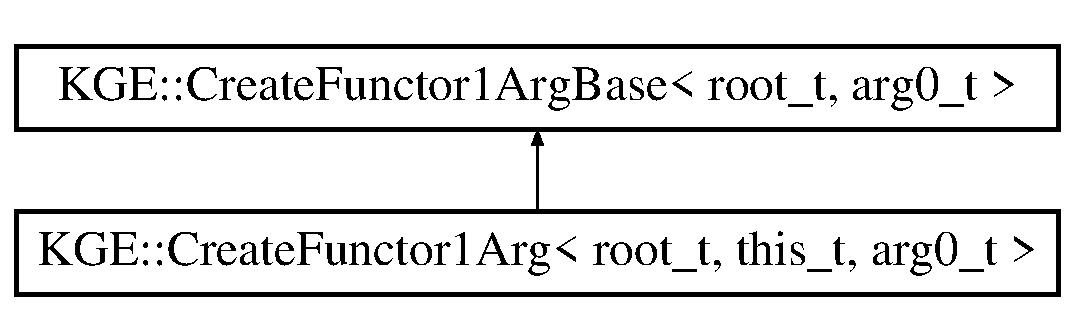
\includegraphics[height=2.000000cm]{class_k_g_e_1_1_create_functor1_arg_base}
\end{center}
\end{figure}
\subsection*{Public Member Functions}
\begin{DoxyCompactItemize}
\item 
\hypertarget{class_k_g_e_1_1_create_functor1_arg_base_af10dd2de0f588c119d16997d0462539a}{virtual root\-\_\-t $\ast$ {\bfseries operator()} (arg0\-\_\-t x\-Arg0)=0}\label{class_k_g_e_1_1_create_functor1_arg_base_af10dd2de0f588c119d16997d0462539a}

\end{DoxyCompactItemize}


The documentation for this class was generated from the following file\-:\begin{DoxyCompactItemize}
\item 
C\-:/\-Users/\-Vit/\-Documents/\-Git\-Hub/\-K\-G\-E/\-K\-G\-E/\-Core/\-Class\-Capabilities/Class\-Factory.\-hpp\end{DoxyCompactItemize}

\hypertarget{class_k_g_e_1_1_create_functor2_args}{\section{K\-G\-E\-:\-:Create\-Functor2\-Args$<$ root\-\_\-t, this\-\_\-t, arg0\-\_\-t, arg1\-\_\-t $>$ Class Template Reference}
\label{class_k_g_e_1_1_create_functor2_args}\index{K\-G\-E\-::\-Create\-Functor2\-Args$<$ root\-\_\-t, this\-\_\-t, arg0\-\_\-t, arg1\-\_\-t $>$@{K\-G\-E\-::\-Create\-Functor2\-Args$<$ root\-\_\-t, this\-\_\-t, arg0\-\_\-t, arg1\-\_\-t $>$}}
}
Inheritance diagram for K\-G\-E\-:\-:Create\-Functor2\-Args$<$ root\-\_\-t, this\-\_\-t, arg0\-\_\-t, arg1\-\_\-t $>$\-:\begin{figure}[H]
\begin{center}
\leavevmode
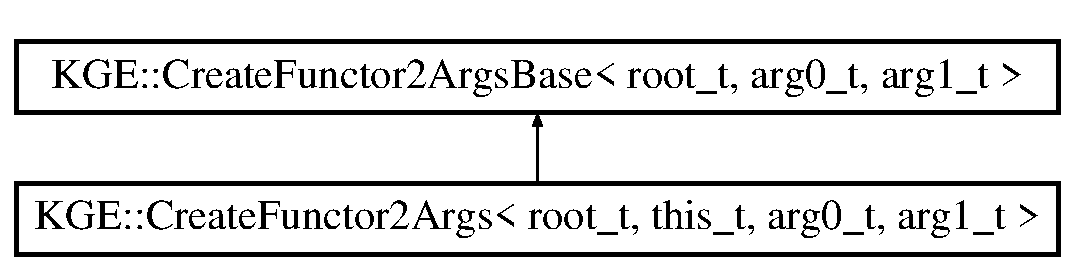
\includegraphics[height=2.000000cm]{class_k_g_e_1_1_create_functor2_args}
\end{center}
\end{figure}
\subsection*{Public Member Functions}
\begin{DoxyCompactItemize}
\item 
\hypertarget{class_k_g_e_1_1_create_functor2_args_a3b0c62d7f1d9c72625e74047cecc5967}{virtual root\-\_\-t $\ast$ {\bfseries operator()} (arg0\-\_\-t x\-Arg0, arg1\-\_\-t x\-Arg1)}\label{class_k_g_e_1_1_create_functor2_args_a3b0c62d7f1d9c72625e74047cecc5967}

\end{DoxyCompactItemize}


The documentation for this class was generated from the following file\-:\begin{DoxyCompactItemize}
\item 
C\-:/\-Users/\-Vit/\-Documents/\-Git\-Hub/\-K\-G\-E/\-K\-G\-E/\-Core/\-Class\-Capabilities/Class\-Factory.\-hpp\end{DoxyCompactItemize}

\hypertarget{class_k_g_e_1_1_create_functor2_args_base}{\section{K\-G\-E\-:\-:Create\-Functor2\-Args\-Base$<$ root\-\_\-t, arg0\-\_\-t, arg1\-\_\-t $>$ Class Template Reference}
\label{class_k_g_e_1_1_create_functor2_args_base}\index{K\-G\-E\-::\-Create\-Functor2\-Args\-Base$<$ root\-\_\-t, arg0\-\_\-t, arg1\-\_\-t $>$@{K\-G\-E\-::\-Create\-Functor2\-Args\-Base$<$ root\-\_\-t, arg0\-\_\-t, arg1\-\_\-t $>$}}
}
Inheritance diagram for K\-G\-E\-:\-:Create\-Functor2\-Args\-Base$<$ root\-\_\-t, arg0\-\_\-t, arg1\-\_\-t $>$\-:\begin{figure}[H]
\begin{center}
\leavevmode
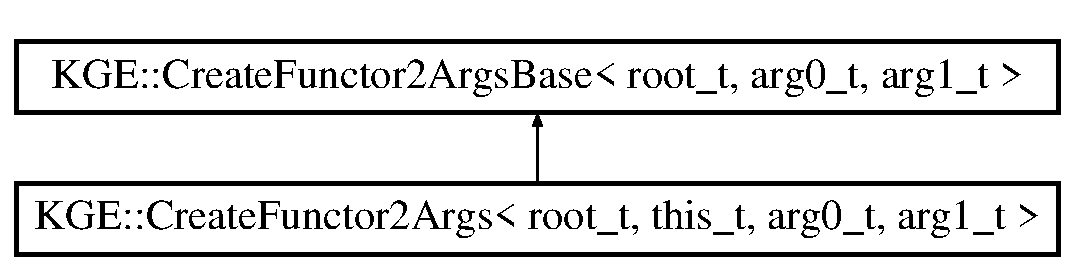
\includegraphics[height=2.000000cm]{class_k_g_e_1_1_create_functor2_args_base}
\end{center}
\end{figure}
\subsection*{Public Member Functions}
\begin{DoxyCompactItemize}
\item 
\hypertarget{class_k_g_e_1_1_create_functor2_args_base_a76c17555b2b35eedeb6ff56bf021e82f}{virtual root\-\_\-t $\ast$ {\bfseries operator()} (arg0\-\_\-t x\-Arg0, arg1\-\_\-t x\-Arg1)=0}\label{class_k_g_e_1_1_create_functor2_args_base_a76c17555b2b35eedeb6ff56bf021e82f}

\end{DoxyCompactItemize}


The documentation for this class was generated from the following file\-:\begin{DoxyCompactItemize}
\item 
C\-:/\-Users/\-Vit/\-Documents/\-Git\-Hub/\-K\-G\-E/\-K\-G\-E/\-Core/\-Class\-Capabilities/Class\-Factory.\-hpp\end{DoxyCompactItemize}

\hypertarget{class_k_g_e_1_1_create_functor_base}{\section{K\-G\-E\-:\-:Create\-Functor\-Base$<$ root\-\_\-t $>$ Class Template Reference}
\label{class_k_g_e_1_1_create_functor_base}\index{K\-G\-E\-::\-Create\-Functor\-Base$<$ root\-\_\-t $>$@{K\-G\-E\-::\-Create\-Functor\-Base$<$ root\-\_\-t $>$}}
}
Inheritance diagram for K\-G\-E\-:\-:Create\-Functor\-Base$<$ root\-\_\-t $>$\-:\begin{figure}[H]
\begin{center}
\leavevmode
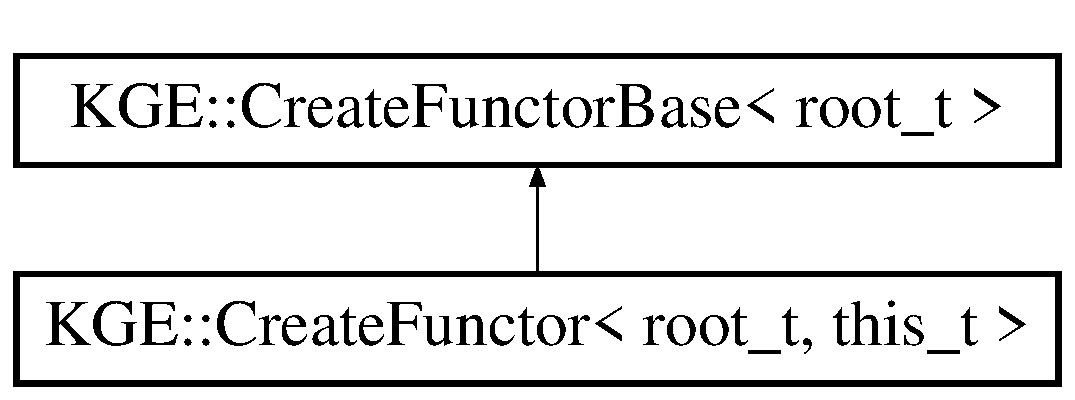
\includegraphics[height=2.000000cm]{class_k_g_e_1_1_create_functor_base}
\end{center}
\end{figure}
\subsection*{Public Member Functions}
\begin{DoxyCompactItemize}
\item 
\hypertarget{class_k_g_e_1_1_create_functor_base_adb47c3c6c9ce98e61ed3906f6f14cce0}{virtual root\-\_\-t $\ast$ {\bfseries operator()} ()=0}\label{class_k_g_e_1_1_create_functor_base_adb47c3c6c9ce98e61ed3906f6f14cce0}

\end{DoxyCompactItemize}


The documentation for this class was generated from the following file\-:\begin{DoxyCompactItemize}
\item 
C\-:/\-Users/\-Vit/\-Documents/\-Git\-Hub/\-K\-G\-E/\-K\-G\-E/\-Core/\-Class\-Capabilities/Class\-Factory.\-hpp\end{DoxyCompactItemize}

\hypertarget{class_k_g_e_1_1_create_functor_x_m_l}{\section{K\-G\-E\-:\-:Create\-Functor\-X\-M\-L$<$ root\-\_\-t, this\-\_\-t $>$ Class Template Reference}
\label{class_k_g_e_1_1_create_functor_x_m_l}\index{K\-G\-E\-::\-Create\-Functor\-X\-M\-L$<$ root\-\_\-t, this\-\_\-t $>$@{K\-G\-E\-::\-Create\-Functor\-X\-M\-L$<$ root\-\_\-t, this\-\_\-t $>$}}
}
Inheritance diagram for K\-G\-E\-:\-:Create\-Functor\-X\-M\-L$<$ root\-\_\-t, this\-\_\-t $>$\-:\begin{figure}[H]
\begin{center}
\leavevmode
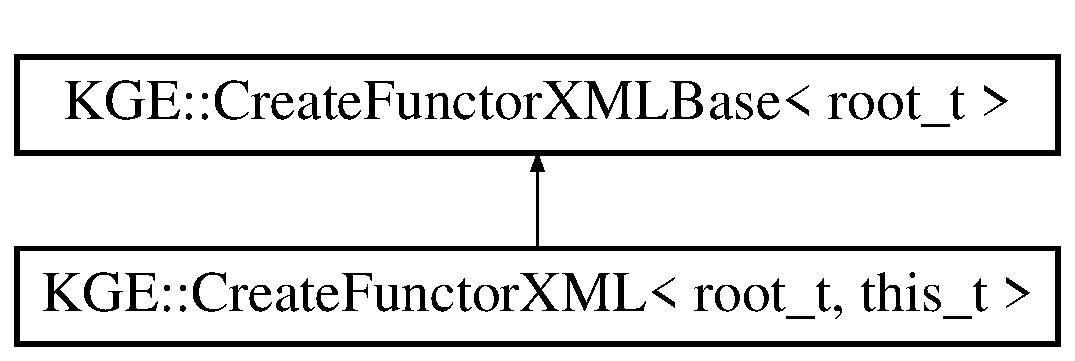
\includegraphics[height=2.000000cm]{class_k_g_e_1_1_create_functor_x_m_l}
\end{center}
\end{figure}
\subsection*{Public Member Functions}
\begin{DoxyCompactItemize}
\item 
\hypertarget{class_k_g_e_1_1_create_functor_x_m_l_a46d109e27e5a68099766f7e231498b94}{virtual root\-\_\-t $\ast$ {\bfseries operator()} (xml\-\_\-node$<$ char $>$ \&x\-Node)}\label{class_k_g_e_1_1_create_functor_x_m_l_a46d109e27e5a68099766f7e231498b94}

\end{DoxyCompactItemize}


The documentation for this class was generated from the following file\-:\begin{DoxyCompactItemize}
\item 
C\-:/\-Users/\-Vit/\-Documents/\-Git\-Hub/\-K\-G\-E/\-K\-G\-E/\-Core/\-Class\-Capabilities/Class\-Factory.\-hpp\end{DoxyCompactItemize}

\hypertarget{class_k_g_e_1_1_create_functor_x_m_l1_arg}{\section{K\-G\-E\-:\-:Create\-Functor\-X\-M\-L1\-Arg$<$ root\-\_\-t, this\-\_\-t, arg0\-\_\-t $>$ Class Template Reference}
\label{class_k_g_e_1_1_create_functor_x_m_l1_arg}\index{K\-G\-E\-::\-Create\-Functor\-X\-M\-L1\-Arg$<$ root\-\_\-t, this\-\_\-t, arg0\-\_\-t $>$@{K\-G\-E\-::\-Create\-Functor\-X\-M\-L1\-Arg$<$ root\-\_\-t, this\-\_\-t, arg0\-\_\-t $>$}}
}
Inheritance diagram for K\-G\-E\-:\-:Create\-Functor\-X\-M\-L1\-Arg$<$ root\-\_\-t, this\-\_\-t, arg0\-\_\-t $>$\-:\begin{figure}[H]
\begin{center}
\leavevmode
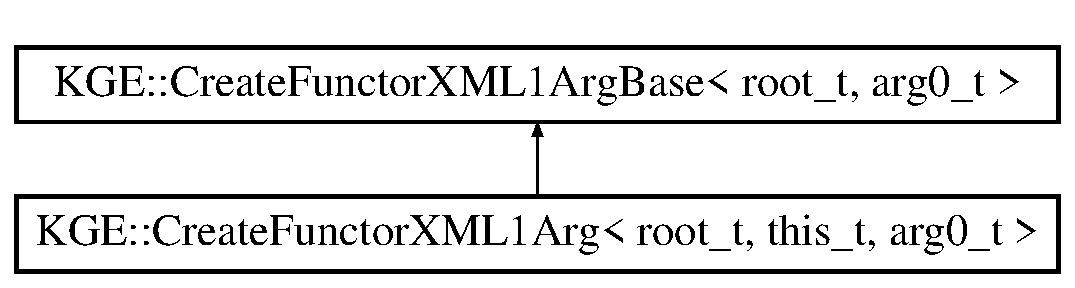
\includegraphics[height=2.000000cm]{class_k_g_e_1_1_create_functor_x_m_l1_arg}
\end{center}
\end{figure}
\subsection*{Public Member Functions}
\begin{DoxyCompactItemize}
\item 
\hypertarget{class_k_g_e_1_1_create_functor_x_m_l1_arg_a4a13152280271c6516e32138971fe560}{virtual root\-\_\-t $\ast$ {\bfseries operator()} (xml\-\_\-node$<$ char $>$ \&x\-Node, arg0\-\_\-t x\-Arg0)}\label{class_k_g_e_1_1_create_functor_x_m_l1_arg_a4a13152280271c6516e32138971fe560}

\end{DoxyCompactItemize}


The documentation for this class was generated from the following file\-:\begin{DoxyCompactItemize}
\item 
C\-:/\-Users/\-Vit/\-Documents/\-Git\-Hub/\-K\-G\-E/\-K\-G\-E/\-Core/\-Class\-Capabilities/Class\-Factory.\-hpp\end{DoxyCompactItemize}

\hypertarget{class_k_g_e_1_1_create_functor_x_m_l1_arg_base}{\section{K\-G\-E\-:\-:Create\-Functor\-X\-M\-L1\-Arg\-Base$<$ root\-\_\-t, arg0\-\_\-t $>$ Class Template Reference}
\label{class_k_g_e_1_1_create_functor_x_m_l1_arg_base}\index{K\-G\-E\-::\-Create\-Functor\-X\-M\-L1\-Arg\-Base$<$ root\-\_\-t, arg0\-\_\-t $>$@{K\-G\-E\-::\-Create\-Functor\-X\-M\-L1\-Arg\-Base$<$ root\-\_\-t, arg0\-\_\-t $>$}}
}
Inheritance diagram for K\-G\-E\-:\-:Create\-Functor\-X\-M\-L1\-Arg\-Base$<$ root\-\_\-t, arg0\-\_\-t $>$\-:\begin{figure}[H]
\begin{center}
\leavevmode
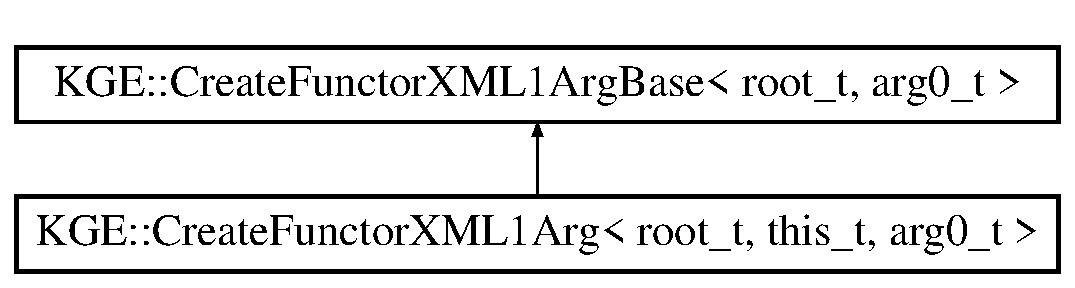
\includegraphics[height=2.000000cm]{class_k_g_e_1_1_create_functor_x_m_l1_arg_base}
\end{center}
\end{figure}
\subsection*{Public Member Functions}
\begin{DoxyCompactItemize}
\item 
\hypertarget{class_k_g_e_1_1_create_functor_x_m_l1_arg_base_a4a9ee65f7b8a81db6b7148ff42cd87bb}{virtual root\-\_\-t $\ast$ {\bfseries operator()} (xml\-\_\-node$<$ char $>$ \&x\-Node, arg0\-\_\-t x\-Arg0)=0}\label{class_k_g_e_1_1_create_functor_x_m_l1_arg_base_a4a9ee65f7b8a81db6b7148ff42cd87bb}

\end{DoxyCompactItemize}


The documentation for this class was generated from the following file\-:\begin{DoxyCompactItemize}
\item 
C\-:/\-Users/\-Vit/\-Documents/\-Git\-Hub/\-K\-G\-E/\-K\-G\-E/\-Core/\-Class\-Capabilities/Class\-Factory.\-hpp\end{DoxyCompactItemize}

\hypertarget{class_k_g_e_1_1_create_functor_x_m_l_base}{\section{K\-G\-E\-:\-:Create\-Functor\-X\-M\-L\-Base$<$ root\-\_\-t $>$ Class Template Reference}
\label{class_k_g_e_1_1_create_functor_x_m_l_base}\index{K\-G\-E\-::\-Create\-Functor\-X\-M\-L\-Base$<$ root\-\_\-t $>$@{K\-G\-E\-::\-Create\-Functor\-X\-M\-L\-Base$<$ root\-\_\-t $>$}}
}
Inheritance diagram for K\-G\-E\-:\-:Create\-Functor\-X\-M\-L\-Base$<$ root\-\_\-t $>$\-:\begin{figure}[H]
\begin{center}
\leavevmode
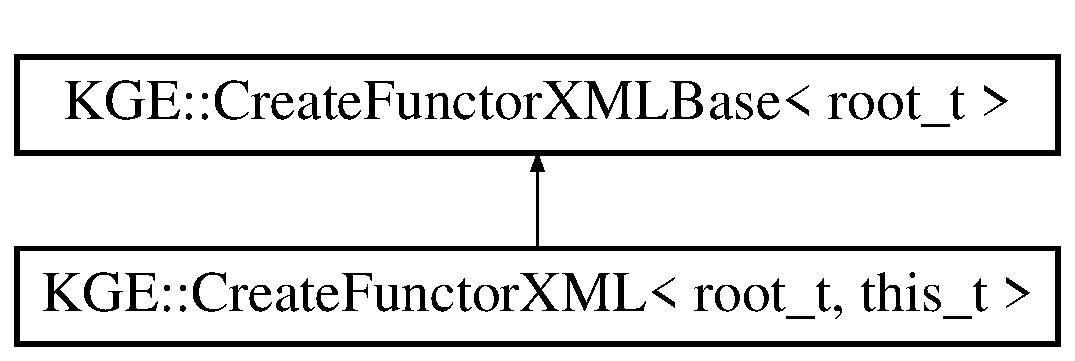
\includegraphics[height=2.000000cm]{class_k_g_e_1_1_create_functor_x_m_l_base}
\end{center}
\end{figure}
\subsection*{Public Member Functions}
\begin{DoxyCompactItemize}
\item 
\hypertarget{class_k_g_e_1_1_create_functor_x_m_l_base_ae974454b91daa10123929a292bc5c8ee}{virtual root\-\_\-t $\ast$ {\bfseries operator()} (xml\-\_\-node$<$ char $>$ \&x\-Node)=0}\label{class_k_g_e_1_1_create_functor_x_m_l_base_ae974454b91daa10123929a292bc5c8ee}

\end{DoxyCompactItemize}


The documentation for this class was generated from the following file\-:\begin{DoxyCompactItemize}
\item 
C\-:/\-Users/\-Vit/\-Documents/\-Git\-Hub/\-K\-G\-E/\-K\-G\-E/\-Core/\-Class\-Capabilities/Class\-Factory.\-hpp\end{DoxyCompactItemize}

\hypertarget{class_k_g_e_1_1_data}{\section{K\-G\-E\-:\-:Data Class Reference}
\label{class_k_g_e_1_1_data}\index{K\-G\-E\-::\-Data@{K\-G\-E\-::\-Data}}
}


{\ttfamily \#include $<$Data.\-hpp$>$}

\subsection*{Public Types}
\begin{DoxyCompactItemize}
\item 
enum \hyperlink{class_k_g_e_1_1_data_acc872a3e856e6d9b554d36d9f534308f}{D\-A\-T\-A\-\_\-\-T\-Y\-P\-E\-S} \{ \\*
{\bfseries U\-N\-S\-E\-T} = 0, 
{\bfseries B\-O\-O\-L}, 
{\bfseries I\-N\-T}, 
{\bfseries U\-I\-N\-T}, 
\\*
{\bfseries F\-L\-O\-A\-T}, 
{\bfseries S\-T\-R\-I\-N\-G}, 
{\bfseries C\-O\-M\-P\-O\-N\-E\-N\-T}, 
{\bfseries H\-A\-S\-H}, 
\\*
{\bfseries V\-E\-C2\-F}, 
{\bfseries R\-E\-N\-D\-E\-R\-T\-A\-R\-G\-E\-T}, 
{\bfseries W\-I\-N\-D\-O\-W}, 
{\bfseries E\-V\-E\-N\-T}
 \}
\begin{DoxyCompactList}\small\item\em \hyperlink{class_k_g_e_1_1_data}{Data} types that the class supports. \end{DoxyCompactList}\end{DoxyCompactItemize}
\subsection*{Public Member Functions}
\begin{DoxyCompactItemize}
\item 
\hypertarget{class_k_g_e_1_1_data_a99e94ff565fe37237ab9fb5b76fbb891}{{\bfseries Data} (bool b\-Value)}\label{class_k_g_e_1_1_data_a99e94ff565fe37237ab9fb5b76fbb891}

\item 
\hypertarget{class_k_g_e_1_1_data_a7d20a85d571fc97595811caad264a617}{{\bfseries Data} (int i\-Value)}\label{class_k_g_e_1_1_data_a7d20a85d571fc97595811caad264a617}

\item 
\hypertarget{class_k_g_e_1_1_data_ac809b9857e669c63df74886c87423f7f}{{\bfseries Data} (u\-\_\-int u\-Value)}\label{class_k_g_e_1_1_data_ac809b9857e669c63df74886c87423f7f}

\item 
\hypertarget{class_k_g_e_1_1_data_a269e9cfaffcd217bc3a7aff6cdb787ac}{{\bfseries Data} (float f\-Value)}\label{class_k_g_e_1_1_data_a269e9cfaffcd217bc3a7aff6cdb787ac}

\item 
\hypertarget{class_k_g_e_1_1_data_a9615c4b192077642dfd501922a8b704e}{{\bfseries Data} (const string \&sz\-Value)}\label{class_k_g_e_1_1_data_a9615c4b192077642dfd501922a8b704e}

\item 
\hypertarget{class_k_g_e_1_1_data_a52c78fd395200fa4d65101aaec82916f}{{\bfseries Data} (\hyperlink{class_k_g_e_1_1_component}{Component} $\ast$px\-Value)}\label{class_k_g_e_1_1_data_a52c78fd395200fa4d65101aaec82916f}

\item 
\hypertarget{class_k_g_e_1_1_data_ae8634ad86f0401f84d1d15f304807dac}{{\bfseries Data} (const \hyperlink{class_k_g_e_1_1_hash}{Hash} \&x\-Value)}\label{class_k_g_e_1_1_data_ae8634ad86f0401f84d1d15f304807dac}

\item 
\hypertarget{class_k_g_e_1_1_data_a1db298fde4e4e49aa53c6ae2090883a5}{{\bfseries Data} (const \hyperlink{struct_k_g_e_1_1_vec2f}{Vec2f} \&x\-Value)}\label{class_k_g_e_1_1_data_a1db298fde4e4e49aa53c6ae2090883a5}

\item 
\hypertarget{class_k_g_e_1_1_data_a88890cc90d6eaa8f3a10f3b7b6a2b871}{{\bfseries Data} (sf\-::\-Render\-Target $\ast$px\-Value)}\label{class_k_g_e_1_1_data_a88890cc90d6eaa8f3a10f3b7b6a2b871}

\item 
\hypertarget{class_k_g_e_1_1_data_a2be099af146b3a57eed1be87bd3a89e6}{{\bfseries Data} (sf\-::\-Window $\ast$px\-Value)}\label{class_k_g_e_1_1_data_a2be099af146b3a57eed1be87bd3a89e6}

\item 
\hypertarget{class_k_g_e_1_1_data_a48d2dd70314d5b87bd99791ead671b28}{{\bfseries Data} (sf\-::\-Event $\ast$px\-Value)}\label{class_k_g_e_1_1_data_a48d2dd70314d5b87bd99791ead671b28}

\item 
\hypertarget{class_k_g_e_1_1_data_a8f08237def00b34cd3bfe420dd3720d3}{{\bfseries Data} (const \hyperlink{class_k_g_e_1_1_data}{Data} \&x\-Copy)}\label{class_k_g_e_1_1_data_a8f08237def00b34cd3bfe420dd3720d3}

\item 
\hypertarget{class_k_g_e_1_1_data_a3b49658c26f1792c8dd4f9da812357f7}{virtual bool $\ast$ {\bfseries As\-Bool} ()}\label{class_k_g_e_1_1_data_a3b49658c26f1792c8dd4f9da812357f7}

\item 
\hypertarget{class_k_g_e_1_1_data_a1900047eebe92f0ef64da5cce90a6d62}{virtual int $\ast$ {\bfseries As\-Int} ()}\label{class_k_g_e_1_1_data_a1900047eebe92f0ef64da5cce90a6d62}

\item 
\hypertarget{class_k_g_e_1_1_data_aebaab43478e1f891772ba4660c28273f}{virtual u\-\_\-int $\ast$ {\bfseries As\-U\-Int} ()}\label{class_k_g_e_1_1_data_aebaab43478e1f891772ba4660c28273f}

\item 
\hypertarget{class_k_g_e_1_1_data_aae0eb1f179567fbfde5cf5c77b133cc1}{virtual float $\ast$ {\bfseries As\-Float} ()}\label{class_k_g_e_1_1_data_aae0eb1f179567fbfde5cf5c77b133cc1}

\item 
\hypertarget{class_k_g_e_1_1_data_aa6bfb5946aa10563fb2318914b1b0842}{virtual string $\ast$ {\bfseries As\-String} ()}\label{class_k_g_e_1_1_data_aa6bfb5946aa10563fb2318914b1b0842}

\item 
\hypertarget{class_k_g_e_1_1_data_ab33682d26e0c5abc5d8f42f223a6248e}{virtual \hyperlink{class_k_g_e_1_1_component}{Component} $\ast$ {\bfseries As\-Component} ()}\label{class_k_g_e_1_1_data_ab33682d26e0c5abc5d8f42f223a6248e}

\item 
\hypertarget{class_k_g_e_1_1_data_a9db175691bcae9f308ccbec74dd30566}{virtual \hyperlink{class_k_g_e_1_1_hash}{Hash} $\ast$ {\bfseries As\-Hash} ()}\label{class_k_g_e_1_1_data_a9db175691bcae9f308ccbec74dd30566}

\item 
\hypertarget{class_k_g_e_1_1_data_abdf66ea9cddd1847cc3ecb09219f4031}{virtual \hyperlink{struct_k_g_e_1_1_vec2f}{Vec2f} $\ast$ {\bfseries As\-Vec2f} ()}\label{class_k_g_e_1_1_data_abdf66ea9cddd1847cc3ecb09219f4031}

\item 
\hypertarget{class_k_g_e_1_1_data_ae8f1d21b0687e36f6cce97a6c3aed5ff}{virtual sf\-::\-Render\-Target $\ast$ {\bfseries As\-Render\-Target} ()}\label{class_k_g_e_1_1_data_ae8f1d21b0687e36f6cce97a6c3aed5ff}

\item 
\hypertarget{class_k_g_e_1_1_data_ac4baaf11bd6728d9cd9d63ff6fe8bbaa}{virtual sf\-::\-Window $\ast$ {\bfseries As\-Window} ()}\label{class_k_g_e_1_1_data_ac4baaf11bd6728d9cd9d63ff6fe8bbaa}

\item 
\hypertarget{class_k_g_e_1_1_data_a30ad6275889382b2d6e8ec30ff00e9f3}{virtual sf\-::\-Event $\ast$ {\bfseries As\-Event} ()}\label{class_k_g_e_1_1_data_a30ad6275889382b2d6e8ec30ff00e9f3}

\item 
\hypertarget{class_k_g_e_1_1_data_ae441b92dfdddc37e9d9f9569f5708dfa}{{\footnotesize template$<$typename type\-\_\-t $>$ }\\type\-\_\-t $\ast$ {\bfseries As\-Type} ()}\label{class_k_g_e_1_1_data_ae441b92dfdddc37e9d9f9569f5708dfa}

\item 
\hypertarget{class_k_g_e_1_1_data_ae067732636c584bb9121b8723e2eb516}{{\footnotesize template$<$$>$ }\\bool $\ast$ {\bfseries As\-Type} ()}\label{class_k_g_e_1_1_data_ae067732636c584bb9121b8723e2eb516}

\item 
\hypertarget{class_k_g_e_1_1_data_a9c93f6bfd0dedc3a5358782deb31ec16}{{\footnotesize template$<$$>$ }\\int $\ast$ {\bfseries As\-Type} ()}\label{class_k_g_e_1_1_data_a9c93f6bfd0dedc3a5358782deb31ec16}

\item 
\hypertarget{class_k_g_e_1_1_data_af99913afa7d34f7136ba1caa5d078ff0}{{\footnotesize template$<$$>$ }\\u\-\_\-int $\ast$ {\bfseries As\-Type} ()}\label{class_k_g_e_1_1_data_af99913afa7d34f7136ba1caa5d078ff0}

\item 
\hypertarget{class_k_g_e_1_1_data_aa7b9df68f1d2a59c54c2d0d17ede27a3}{{\footnotesize template$<$$>$ }\\float $\ast$ {\bfseries As\-Type} ()}\label{class_k_g_e_1_1_data_aa7b9df68f1d2a59c54c2d0d17ede27a3}

\item 
\hypertarget{class_k_g_e_1_1_data_a0df677588b351f1faf12d28be6179f51}{{\footnotesize template$<$$>$ }\\string $\ast$ {\bfseries As\-Type} ()}\label{class_k_g_e_1_1_data_a0df677588b351f1faf12d28be6179f51}

\item 
\hypertarget{class_k_g_e_1_1_data_ae4b311a61df702ba64e9af9d9a1f9d09}{{\footnotesize template$<$$>$ }\\\hyperlink{class_k_g_e_1_1_component}{Component} $\ast$ {\bfseries As\-Type} ()}\label{class_k_g_e_1_1_data_ae4b311a61df702ba64e9af9d9a1f9d09}

\item 
\hypertarget{class_k_g_e_1_1_data_a20d87bed9791473bdec7bdf5f46cff47}{{\footnotesize template$<$$>$ }\\\hyperlink{class_k_g_e_1_1_hash}{Hash} $\ast$ {\bfseries As\-Type} ()}\label{class_k_g_e_1_1_data_a20d87bed9791473bdec7bdf5f46cff47}

\item 
\hypertarget{class_k_g_e_1_1_data_ae30d13c2899a40892fd22bd3646e8dd6}{{\footnotesize template$<$$>$ }\\\hyperlink{struct_k_g_e_1_1_vec2f}{Vec2f} $\ast$ {\bfseries As\-Type} ()}\label{class_k_g_e_1_1_data_ae30d13c2899a40892fd22bd3646e8dd6}

\item 
\hypertarget{class_k_g_e_1_1_data_a919532108aa4b35f536e9fe64fe90f15}{{\footnotesize template$<$$>$ }\\sf\-::\-Render\-Target $\ast$ {\bfseries As\-Type} ()}\label{class_k_g_e_1_1_data_a919532108aa4b35f536e9fe64fe90f15}

\item 
\hypertarget{class_k_g_e_1_1_data_a78a699ce8e5f10b699621fe57024683c}{{\footnotesize template$<$$>$ }\\sf\-::\-Window $\ast$ {\bfseries As\-Type} ()}\label{class_k_g_e_1_1_data_a78a699ce8e5f10b699621fe57024683c}

\item 
\hypertarget{class_k_g_e_1_1_data_a83804415d4aa5d20e98aa6cd1986b111}{{\footnotesize template$<$$>$ }\\sf\-::\-Event $\ast$ {\bfseries As\-Type} ()}\label{class_k_g_e_1_1_data_a83804415d4aa5d20e98aa6cd1986b111}

\item 
\hypertarget{class_k_g_e_1_1_data_a8a82c58b3228fde51e059080a8bf5df7}{virtual \hyperlink{class_k_g_e_1_1_data_acc872a3e856e6d9b554d36d9f534308f}{D\-A\-T\-A\-\_\-\-T\-Y\-P\-E\-S} {\bfseries Get\-Type} () const }\label{class_k_g_e_1_1_data_a8a82c58b3228fde51e059080a8bf5df7}

\item 
\hypertarget{class_k_g_e_1_1_data_a8333dd8ae22ac619712adbdb83c09800}{bool \hyperlink{class_k_g_e_1_1_data_a8333dd8ae22ac619712adbdb83c09800}{operator!=} (const \hyperlink{class_k_g_e_1_1_data}{Data} \&x\-R\-H\-S) const }\label{class_k_g_e_1_1_data_a8333dd8ae22ac619712adbdb83c09800}

\begin{DoxyCompactList}\small\item\em Overloaded inequality operator\-: implemented in terms of the equality operator. \end{DoxyCompactList}\item 
\hypertarget{class_k_g_e_1_1_data_ae2b3bf0593f3d9559204ed12b105c7c5}{bool \hyperlink{class_k_g_e_1_1_data_ae2b3bf0593f3d9559204ed12b105c7c5}{operator==} (const \hyperlink{class_k_g_e_1_1_data}{Data} \&x\-R\-H\-S) const }\label{class_k_g_e_1_1_data_ae2b3bf0593f3d9559204ed12b105c7c5}

\begin{DoxyCompactList}\small\item\em Overloaded equality operator\-: returns false if both \hyperlink{class_k_g_e_1_1_data}{Data} instances store different types or. \end{DoxyCompactList}\end{DoxyCompactItemize}
\subsection*{Protected Attributes}
\begin{DoxyCompactItemize}
\item 
\hypertarget{class_k_g_e_1_1_data_a8880e6ed5a798e09c917317afa337e01}{\begin{tabbing}
xx\=xx\=xx\=xx\=xx\=xx\=xx\=xx\=xx\=\kill
union \{\\
\hypertarget{union_k_g_e_1_1_data_1_1@0_a4d0dd8b60abb46df1cd1744275ef1da7}{\>bool {\bfseries b}\\
\hypertarget{union_k_g_e_1_1_data_1_1@0_ad096f23d39e860f9d6a001273a0b232b}{\>int {\bfseries i}\\
\hypertarget{union_k_g_e_1_1_data_1_1@0_a4bc97770313d84af56ea6b59d4179d99}{\>u\_int {\bfseries u}\\
\hypertarget{union_k_g_e_1_1_data_1_1@0_a0eefe1ffc4136b03ee2205a6333fca5f}{\>float {\bfseries f}\\
\hypertarget{union_k_g_e_1_1_data_1_1@0_aa43bfe02e7762c9efad8b0b48e4a7664}{\>\hyperlink{class_k_g_e_1_1_component}{Component} $\ast$ {\bfseries c}\\
\hypertarget{union_k_g_e_1_1_data_1_1@0_aafe8eee1150c1ad3a9e0651a965a2f36}{\>sf::RenderTarget $\ast$ {\bfseries rt}\\
\hypertarget{union_k_g_e_1_1_data_1_1@0_af51df1c980e8824c0cb0f0306111f87a}{\>sf::Window $\ast$ {\bfseries w}\\
\hypertarget{union_k_g_e_1_1_data_1_1@0_ae51fe96bcc5458b6c6f0590eb1a729e3}{\>sf::Event $\ast$ {\bfseries e}\\
\} {\bfseries m\_xProperty}}\label{class_k_g_e_1_1_data_a8880e6ed5a798e09c917317afa337e01}
\\

\end{tabbing}\item 
\hypertarget{class_k_g_e_1_1_data_a7a507ee6985488d936a2270c96e26cd6}{string {\bfseries m\-\_\-x\-Property\-S}}\label{class_k_g_e_1_1_data_a7a507ee6985488d936a2270c96e26cd6}

\item 
\hypertarget{class_k_g_e_1_1_data_ab3d1e90f24431fdaddf7787f5a808095}{\hyperlink{class_k_g_e_1_1_hash}{Hash} {\bfseries m\-\_\-x\-Property\-H}}\label{class_k_g_e_1_1_data_ab3d1e90f24431fdaddf7787f5a808095}

\item 
\hypertarget{class_k_g_e_1_1_data_ad0f7ebed1eff5795e4e805ee0cd473de}{\hyperlink{struct_k_g_e_1_1_vec2f}{Vec2f} {\bfseries m\-\_\-x\-Property\-V}}\label{class_k_g_e_1_1_data_ad0f7ebed1eff5795e4e805ee0cd473de}

\item 
\hypertarget{class_k_g_e_1_1_data_abc11b0d544cf2f58cf612cb611125760}{\hyperlink{class_k_g_e_1_1_data_acc872a3e856e6d9b554d36d9f534308f}{D\-A\-T\-A\-\_\-\-T\-Y\-P\-E\-S} {\bfseries m\-\_\-e\-Type}}\label{class_k_g_e_1_1_data_abc11b0d544cf2f58cf612cb611125760}

\end{DoxyCompactItemize}


\subsection{Detailed Description}
\hyperlink{class_k_g_e_1_1_data}{K\-G\-E\-::\-Data} This wrapper class designed to store any type of data. To find the data types supported, please see the \hyperlink{class_k_g_e_1_1_data_acc872a3e856e6d9b554d36d9f534308f}{K\-G\-E\-::\-Data\-::\-D\-A\-T\-A\-\_\-\-T\-Y\-P\-E\-S} enum values. An instance of this class can only store one type of data, thus retrieving an int as a bool is N\-O\-T supported. the getters of this class always return a pointer to the data, and if the requested type does not match the type of the stored data, N\-U\-L\-L is returned. 

The documentation for this class was generated from the following files\-:\begin{DoxyCompactItemize}
\item 
C\-:/\-Users/\-Vit/\-Documents/\-Git\-Hub/\-K\-G\-E/\-K\-G\-E/\-Core/\-Data/Data.\-hpp\item 
C\-:/\-Users/\-Vit/\-Documents/\-Git\-Hub/\-K\-G\-E/\-K\-G\-E/\-Core/\-Data/Data.\-cpp\end{DoxyCompactItemize}

\hypertarget{class_k_g_e_1_1_event}{\section{K\-G\-E\-:\-:Event$<$ owner\-\_\-t $>$ Class Template Reference}
\label{class_k_g_e_1_1_event}\index{K\-G\-E\-::\-Event$<$ owner\-\_\-t $>$@{K\-G\-E\-::\-Event$<$ owner\-\_\-t $>$}}
}
\subsection*{Public Types}
\begin{DoxyCompactItemize}
\item 
\hypertarget{class_k_g_e_1_1_event_abafaf93279c4dab788af267b02e56303}{typedef unordered\-\_\-map$<$ \hyperlink{class_k_g_e_1_1_hash}{Hash}, \\*
\hyperlink{class_k_g_e_1_1_event}{Event}$<$ owner\-\_\-t $>$\\*
 $\ast$, \hyperlink{struct_k_g_e_1_1_hash_1_1_hasher}{Hash\-::\-Hasher} $>$ {\bfseries collection\-\_\-t}}\label{class_k_g_e_1_1_event_abafaf93279c4dab788af267b02e56303}

\item 
\hypertarget{class_k_g_e_1_1_event_abe78630172ef261fcbc6b8fd04e996a8}{typedef pair$<$ \hyperlink{class_k_g_e_1_1_hash}{Hash}, \hyperlink{class_k_g_e_1_1_event}{Event}\\*
$<$ owner\-\_\-t $>$ $\ast$ $>$ {\bfseries collectionpair\-\_\-t}}\label{class_k_g_e_1_1_event_abe78630172ef261fcbc6b8fd04e996a8}

\end{DoxyCompactItemize}
\subsection*{Public Member Functions}
\begin{DoxyCompactItemize}
\item 
\hypertarget{class_k_g_e_1_1_event_a718fe1b0a1a4ff9768dea405485844ff}{{\bfseries Event} (const \hyperlink{class_k_g_e_1_1_hash}{Hash} \&x\-Hash, owner\-\_\-t \&x\-Caller, std\-::function$<$ void(eventparams\-\_\-t \&)$>$ x\-Callback)}\label{class_k_g_e_1_1_event_a718fe1b0a1a4ff9768dea405485844ff}

\item 
\hypertarget{class_k_g_e_1_1_event_a731391dcb56fc726f203ce2f0ce18d10}{void {\bfseries Register\-Signal} (\hyperlink{class_k_g_e_1_1_event_signal}{Event\-Signal}$<$ owner\-\_\-t $>$ $\ast$px\-Signal)}\label{class_k_g_e_1_1_event_a731391dcb56fc726f203ce2f0ce18d10}

\item 
\hypertarget{class_k_g_e_1_1_event_a7a62b2d97ffe3c87455160b257c2b116}{void {\bfseries Unregister\-Signal} (\hyperlink{class_k_g_e_1_1_event_signal}{Event\-Signal}$<$ owner\-\_\-t $>$ $\ast$px\-Signal)}\label{class_k_g_e_1_1_event_a7a62b2d97ffe3c87455160b257c2b116}

\item 
\hypertarget{class_k_g_e_1_1_event_a3e632d4e01b37e0f3c3fa404d73bb7fc}{void {\bfseries Execute} (eventparams\-\_\-t \&x\-Event\-Parameters)}\label{class_k_g_e_1_1_event_a3e632d4e01b37e0f3c3fa404d73bb7fc}

\item 
\hypertarget{class_k_g_e_1_1_event_a4f38ca1d86b9d319dd591eaf6cc2999a}{virtual const \hyperlink{class_k_g_e_1_1_hash}{Hash} \& {\bfseries Get\-Hash} () const }\label{class_k_g_e_1_1_event_a4f38ca1d86b9d319dd591eaf6cc2999a}

\end{DoxyCompactItemize}
\subsection*{Protected Attributes}
\begin{DoxyCompactItemize}
\item 
\hypertarget{class_k_g_e_1_1_event_a896140405a443b76b39503fc29adcd16}{\hyperlink{class_k_g_e_1_1_hash}{Hash} {\bfseries m\-\_\-x\-Hash}}\label{class_k_g_e_1_1_event_a896140405a443b76b39503fc29adcd16}

\item 
\hypertarget{class_k_g_e_1_1_event_a510003f7bed85cfdbca5400105576832}{owner\-\_\-t \& {\bfseries m\-\_\-x\-Caller}}\label{class_k_g_e_1_1_event_a510003f7bed85cfdbca5400105576832}

\item 
\hypertarget{class_k_g_e_1_1_event_ae0ecaf668869d285e28a5ecce70b634d}{std\-::function$<$ void(eventparams\-\_\-t \&)$>$ {\bfseries m\-\_\-x\-Callback}}\label{class_k_g_e_1_1_event_ae0ecaf668869d285e28a5ecce70b634d}

\item 
\hypertarget{class_k_g_e_1_1_event_a25cb534b76a8d499622660e332692800}{std\-::set$<$ \hyperlink{class_k_g_e_1_1_event_signal}{Event\-Signal}$<$ owner\-\_\-t $>$\\*
 $\ast$, typename \hyperlink{class_k_g_e_1_1_event_signal}{Event\-Signal}\\*
$<$ owner\-\_\-t $>$\-::Comparer $>$ {\bfseries m\-\_\-x\-Signals}}\label{class_k_g_e_1_1_event_a25cb534b76a8d499622660e332692800}

\end{DoxyCompactItemize}


The documentation for this class was generated from the following file\-:\begin{DoxyCompactItemize}
\item 
C\-:/\-Users/\-Vit/\-Documents/\-Git\-Hub/\-K\-G\-E/\-K\-G\-E/\-Core/\-Class\-Capabilities/Events.\-hpp\end{DoxyCompactItemize}

\hypertarget{class_k_g_e_1_1_event_signal}{\section{K\-G\-E\-:\-:Event\-Signal$<$ owner\-\_\-t $>$ Class Template Reference}
\label{class_k_g_e_1_1_event_signal}\index{K\-G\-E\-::\-Event\-Signal$<$ owner\-\_\-t $>$@{K\-G\-E\-::\-Event\-Signal$<$ owner\-\_\-t $>$}}
}
\subsection*{Classes}
\begin{DoxyCompactItemize}
\item 
struct \hyperlink{struct_k_g_e_1_1_event_signal_1_1_comparer}{Comparer}
\end{DoxyCompactItemize}
\subsection*{Public Member Functions}
\begin{DoxyCompactItemize}
\item 
\hypertarget{class_k_g_e_1_1_event_signal_a121dfd0a1f2cafd3bc803bbc3e3cacea}{{\bfseries Event\-Signal} (owner\-\_\-t \&x\-Owner)}\label{class_k_g_e_1_1_event_signal_a121dfd0a1f2cafd3bc803bbc3e3cacea}

\item 
\hypertarget{class_k_g_e_1_1_event_signal_a68e673396d68e99a4d0415cccfac5d82}{{\bfseries Event\-Signal} (xml\-\_\-node$<$ char $>$ \&x\-Node, owner\-\_\-t \&x\-Owner)}\label{class_k_g_e_1_1_event_signal_a68e673396d68e99a4d0415cccfac5d82}

\item 
\hypertarget{class_k_g_e_1_1_event_signal_a2f98b89b96d1e784dbd45d3c6dc5328f}{void {\bfseries Activate} ()}\label{class_k_g_e_1_1_event_signal_a2f98b89b96d1e784dbd45d3c6dc5328f}

\item 
\hypertarget{class_k_g_e_1_1_event_signal_a3bd5d17f63a0f2829fb9d6584bf548ce}{void {\bfseries Deactivate} ()}\label{class_k_g_e_1_1_event_signal_a3bd5d17f63a0f2829fb9d6584bf548ce}

\item 
\hypertarget{class_k_g_e_1_1_event_signal_a33ff8d1fc42a054923e763a2e7d3a334}{void {\bfseries Execute} (eventparams\-\_\-t \&x\-Params)}\label{class_k_g_e_1_1_event_signal_a33ff8d1fc42a054923e763a2e7d3a334}

\item 
\hypertarget{class_k_g_e_1_1_event_signal_aa654f733e993ec10a5541d9b61564101}{void {\bfseries Set\-Priority} (float f\-Priority)}\label{class_k_g_e_1_1_event_signal_aa654f733e993ec10a5541d9b61564101}

\item 
\hypertarget{class_k_g_e_1_1_event_signal_a9584569f24029b389e55c5e0feae1cda}{float {\bfseries Get\-Priority} () const }\label{class_k_g_e_1_1_event_signal_a9584569f24029b389e55c5e0feae1cda}

\end{DoxyCompactItemize}
\subsection*{Protected Member Functions}
\begin{DoxyCompactItemize}
\item 
\hypertarget{class_k_g_e_1_1_event_signal_adf65006b13b9dbb167490670879c9669}{void {\bfseries Process\-Trigger} (xml\-\_\-attribute$<$ char $>$ \&x\-Event)}\label{class_k_g_e_1_1_event_signal_adf65006b13b9dbb167490670879c9669}

\item 
\hypertarget{class_k_g_e_1_1_event_signal_a8dbace77a099c11639225f133020af3d}{void {\bfseries Process\-Target} (xml\-\_\-attribute$<$ char $>$ \&x\-Event)}\label{class_k_g_e_1_1_event_signal_a8dbace77a099c11639225f133020af3d}

\item 
\hypertarget{class_k_g_e_1_1_event_signal_a54a97ca4837f3e2131ebf962d59d4002}{void {\bfseries Process\-Parameter} (xml\-\_\-node$<$ char $>$ \&x\-Parameter)}\label{class_k_g_e_1_1_event_signal_a54a97ca4837f3e2131ebf962d59d4002}

\item 
\hypertarget{class_k_g_e_1_1_event_signal_a055beb2edc99f655ed74dec80464d953}{void {\bfseries Process\-Priority} (xml\-\_\-attribute$<$ char $>$ \&x\-Priority)}\label{class_k_g_e_1_1_event_signal_a055beb2edc99f655ed74dec80464d953}

\end{DoxyCompactItemize}
\subsection*{Protected Attributes}
\begin{DoxyCompactItemize}
\item 
\hypertarget{class_k_g_e_1_1_event_signal_a40cc0e1308169ee30393e24636ea33c7}{owner\-\_\-t \& {\bfseries m\-\_\-x\-Owner}}\label{class_k_g_e_1_1_event_signal_a40cc0e1308169ee30393e24636ea33c7}

\item 
\hypertarget{class_k_g_e_1_1_event_signal_a24a350f8c112e8c578dc072e6a9054ca}{float {\bfseries m\-\_\-f\-Priority}}\label{class_k_g_e_1_1_event_signal_a24a350f8c112e8c578dc072e6a9054ca}

\item 
\hypertarget{class_k_g_e_1_1_event_signal_ae9ef131e2e10e146de7b72e2048424b2}{const char $\ast$ {\bfseries m\-\_\-sz\-Trigger\-Path}}\label{class_k_g_e_1_1_event_signal_ae9ef131e2e10e146de7b72e2048424b2}

\item 
\hypertarget{class_k_g_e_1_1_event_signal_a37e072a9c265912a8a602982440f128b}{\hyperlink{class_k_g_e_1_1_event}{Event}$<$ owner\-\_\-t $>$ $\ast$ {\bfseries m\-\_\-px\-Trigger\-Event}}\label{class_k_g_e_1_1_event_signal_a37e072a9c265912a8a602982440f128b}

\item 
\hypertarget{class_k_g_e_1_1_event_signal_a6732a2177dd72e19ed5222f4e7012392}{const char $\ast$ {\bfseries m\-\_\-sz\-Target\-Path}}\label{class_k_g_e_1_1_event_signal_a6732a2177dd72e19ed5222f4e7012392}

\item 
\hypertarget{class_k_g_e_1_1_event_signal_a717aff13f897a7acda5eeb59a5364d06}{\hyperlink{class_k_g_e_1_1_event}{Event}$<$ owner\-\_\-t $>$ $\ast$ {\bfseries m\-\_\-px\-Target\-Event}}\label{class_k_g_e_1_1_event_signal_a717aff13f897a7acda5eeb59a5364d06}

\item 
\hypertarget{class_k_g_e_1_1_event_signal_a4336b588f706964e78a4e54ad32a9165}{eventparams\-\_\-t {\bfseries m\-\_\-x\-Parameters}}\label{class_k_g_e_1_1_event_signal_a4336b588f706964e78a4e54ad32a9165}

\end{DoxyCompactItemize}


The documentation for this class was generated from the following file\-:\begin{DoxyCompactItemize}
\item 
C\-:/\-Users/\-Vit/\-Documents/\-Git\-Hub/\-K\-G\-E/\-K\-G\-E/\-Core/\-Class\-Capabilities/Event\-Signal.\-hpp\end{DoxyCompactItemize}

\hypertarget{class_k_g_e_1_1_font_manager}{\section{K\-G\-E\-:\-:Font\-Manager Class Reference}
\label{class_k_g_e_1_1_font_manager}\index{K\-G\-E\-::\-Font\-Manager@{K\-G\-E\-::\-Font\-Manager}}
}
\subsection*{Public Member Functions}
\begin{DoxyCompactItemize}
\item 
\hypertarget{class_k_g_e_1_1_font_manager_aeabc37b99ae4a625e3a95939deccc5ca}{sf\-::\-Font $\ast$ {\bfseries Load\-Font} (const std\-::string \&sz\-File\-Name)}\label{class_k_g_e_1_1_font_manager_aeabc37b99ae4a625e3a95939deccc5ca}

\item 
\hypertarget{class_k_g_e_1_1_font_manager_a0c5c972ea0d8e338e782de13b9b8ed08}{sf\-::\-Font $\ast$ {\bfseries Get\-Font} (const \hyperlink{class_k_g_e_1_1_hash}{Hash} \&x\-Hash)}\label{class_k_g_e_1_1_font_manager_a0c5c972ea0d8e338e782de13b9b8ed08}

\item 
\hypertarget{class_k_g_e_1_1_font_manager_a9961469754e993e6b6e3f35be5cdd276}{void {\bfseries Release\-Font} (const \hyperlink{class_k_g_e_1_1_hash}{Hash} \&x\-Hash)}\label{class_k_g_e_1_1_font_manager_a9961469754e993e6b6e3f35be5cdd276}

\item 
\hypertarget{class_k_g_e_1_1_font_manager_aa15a96333b820a1738b43e74a40ffd36}{void {\bfseries Release\-Font} (sf\-::\-Font $\ast$px\-Font)}\label{class_k_g_e_1_1_font_manager_aa15a96333b820a1738b43e74a40ffd36}

\end{DoxyCompactItemize}
\subsection*{Static Public Member Functions}
\begin{DoxyCompactItemize}
\item 
\hypertarget{class_k_g_e_1_1_font_manager_a57a02b370049d20dd6fc4126b0619f04}{static \hyperlink{class_k_g_e_1_1_font_manager}{Font\-Manager} \& {\bfseries Get} ()}\label{class_k_g_e_1_1_font_manager_a57a02b370049d20dd6fc4126b0619f04}

\end{DoxyCompactItemize}
\subsection*{Protected Attributes}
\begin{DoxyCompactItemize}
\item 
\hypertarget{class_k_g_e_1_1_font_manager_a565480a213fdace5b4df4f1377734b21}{fontcollection\-\_\-t {\bfseries m\-\_\-x\-Font\-List}}\label{class_k_g_e_1_1_font_manager_a565480a213fdace5b4df4f1377734b21}

\end{DoxyCompactItemize}


The documentation for this class was generated from the following files\-:\begin{DoxyCompactItemize}
\item 
C\-:/\-Users/\-Vit/\-Documents/\-Git\-Hub/\-K\-G\-E/\-K\-G\-E/\-Core/\-Resources/Font\-Manager.\-hpp\item 
C\-:/\-Users/\-Vit/\-Documents/\-Git\-Hub/\-K\-G\-E/\-K\-G\-E/\-Core/\-Resources/Font\-Manager.\-cpp\end{DoxyCompactItemize}

\hypertarget{class_k_g_e_1_1_hash}{\section{K\-G\-E\-:\-:Hash Class Reference}
\label{class_k_g_e_1_1_hash}\index{K\-G\-E\-::\-Hash@{K\-G\-E\-::\-Hash}}
}
\subsection*{Classes}
\begin{DoxyCompactItemize}
\item 
struct \hyperlink{struct_k_g_e_1_1_hash_1_1_hasher}{Hasher}
\end{DoxyCompactItemize}
\subsection*{Public Member Functions}
\begin{DoxyCompactItemize}
\item 
\hypertarget{class_k_g_e_1_1_hash_ad85f452a0af194998327bbbd3892c57c}{{\bfseries Hash} (const string \&sz\-Hash\-String)}\label{class_k_g_e_1_1_hash_ad85f452a0af194998327bbbd3892c57c}

\item 
\hypertarget{class_k_g_e_1_1_hash_a82100dca30efafffac59501a9857442c}{{\bfseries Hash} (unsigned int u\-Hash\-Value)}\label{class_k_g_e_1_1_hash_a82100dca30efafffac59501a9857442c}

\item 
\hypertarget{class_k_g_e_1_1_hash_ae05a3545183bba26bff3af69f064a34d}{{\bfseries Hash} (const \hyperlink{class_k_g_e_1_1_hash}{Hash} \&x\-Copy)}\label{class_k_g_e_1_1_hash_ae05a3545183bba26bff3af69f064a34d}

\item 
\hypertarget{class_k_g_e_1_1_hash_ad09667dae0b9206ac5ec0cf24eb043ba}{void {\bfseries operator=} (const \hyperlink{class_k_g_e_1_1_hash}{Hash} \&b)}\label{class_k_g_e_1_1_hash_ad09667dae0b9206ac5ec0cf24eb043ba}

\item 
\hypertarget{class_k_g_e_1_1_hash_aea2eef8e02fd5a4d46f6c489b6224991}{void {\bfseries operator=} (const string \&b)}\label{class_k_g_e_1_1_hash_aea2eef8e02fd5a4d46f6c489b6224991}

\item 
\hypertarget{class_k_g_e_1_1_hash_a00a4b2822d7f3ce7e9ebc005de023657}{void {\bfseries operator+=} (const string \&b)}\label{class_k_g_e_1_1_hash_a00a4b2822d7f3ce7e9ebc005de023657}

\item 
\hypertarget{class_k_g_e_1_1_hash_abc4d60912c38a6f94faf6c403c8f1c2c}{void {\bfseries operator+=} (char b)}\label{class_k_g_e_1_1_hash_abc4d60912c38a6f94faf6c403c8f1c2c}

\item 
\hypertarget{class_k_g_e_1_1_hash_a7888fa46fb3c0471597b42cf52f3e0e0}{bool {\bfseries operator==} (const \hyperlink{class_k_g_e_1_1_hash}{Hash} \&b) const }\label{class_k_g_e_1_1_hash_a7888fa46fb3c0471597b42cf52f3e0e0}

\item 
\hypertarget{class_k_g_e_1_1_hash_a084211ef4310ba2d7e2880d8aa856eb9}{bool {\bfseries operator!=} (const \hyperlink{class_k_g_e_1_1_hash}{Hash} \&b) const }\label{class_k_g_e_1_1_hash_a084211ef4310ba2d7e2880d8aa856eb9}

\item 
\hypertarget{class_k_g_e_1_1_hash_a48a84591f36df5dc29bc4b353cd24d0d}{bool {\bfseries operator$<$} (const \hyperlink{class_k_g_e_1_1_hash}{Hash} \&b) const }\label{class_k_g_e_1_1_hash_a48a84591f36df5dc29bc4b353cd24d0d}

\item 
\hypertarget{class_k_g_e_1_1_hash_ab3673c02ea07f72ee43f7495b889af5b}{\hyperlink{class_k_g_e_1_1_hash}{Hash} {\bfseries operator+} (const string \&b) const }\label{class_k_g_e_1_1_hash_ab3673c02ea07f72ee43f7495b889af5b}

\item 
\hypertarget{class_k_g_e_1_1_hash_afc6d39e74c0200a8a4d25ee2a5aa55f6}{{\footnotesize template$<$typename I\-N\-\_\-\-T $>$ }\\\hyperlink{class_k_g_e_1_1_hash}{Hash} \& {\bfseries operator$<$$<$} (const I\-N\-\_\-\-T \&x\-In)}\label{class_k_g_e_1_1_hash_afc6d39e74c0200a8a4d25ee2a5aa55f6}

\item 
\hypertarget{class_k_g_e_1_1_hash_a50fbb3432c9bff1ca824881c99962baa}{bool {\bfseries From\-Token} (char c\-Seperator, const char $\ast$\&sz\-String)}\label{class_k_g_e_1_1_hash_a50fbb3432c9bff1ca824881c99962baa}

\item 
\hypertarget{class_k_g_e_1_1_hash_a2e702fe8b3fbf91c78a205b99599029e}{unsigned int {\bfseries Get\-Hash} () const }\label{class_k_g_e_1_1_hash_a2e702fe8b3fbf91c78a205b99599029e}

\item 
\hypertarget{class_k_g_e_1_1_hash_a0df372f141f5a28e430e388ed845aee1}{void {\bfseries Invalidate} ()}\label{class_k_g_e_1_1_hash_a0df372f141f5a28e430e388ed845aee1}

\item 
\hypertarget{class_k_g_e_1_1_hash_a8bfa65740d0ff904a1aa319263c3d4a0}{bool {\bfseries Is\-Invalid} () const }\label{class_k_g_e_1_1_hash_a8bfa65740d0ff904a1aa319263c3d4a0}

\end{DoxyCompactItemize}
\subsection*{Static Public Attributes}
\begin{DoxyCompactItemize}
\item 
\hypertarget{class_k_g_e_1_1_hash_a9912d509163e033a5e3624e533cc81f4}{static const unsigned int {\bfseries U\-N\-S\-E\-T} = 0}\label{class_k_g_e_1_1_hash_a9912d509163e033a5e3624e533cc81f4}

\end{DoxyCompactItemize}
\subsection*{Protected Member Functions}
\begin{DoxyCompactItemize}
\item 
\hypertarget{class_k_g_e_1_1_hash_a7cdf41c18270d407c24ee113e6ba3ce1}{void {\bfseries Set\-Hash} (const string \&sz\-Hash\-String)}\label{class_k_g_e_1_1_hash_a7cdf41c18270d407c24ee113e6ba3ce1}

\item 
\hypertarget{class_k_g_e_1_1_hash_aa2e106049f750ccc822cf7f25f129fd0}{void {\bfseries Concatenate\-Hash} (const std\-::string \&sz\-Hash\-String)}\label{class_k_g_e_1_1_hash_aa2e106049f750ccc822cf7f25f129fd0}

\item 
\hypertarget{class_k_g_e_1_1_hash_a93caac41c8742403562c9e7f4fa34f9f}{void {\bfseries Concatenate\-Hash} (char c\-Char)}\label{class_k_g_e_1_1_hash_a93caac41c8742403562c9e7f4fa34f9f}

\end{DoxyCompactItemize}
\subsection*{Protected Attributes}
\begin{DoxyCompactItemize}
\item 
\hypertarget{class_k_g_e_1_1_hash_a7f69224148adb995aed2eff1e5ba9f29}{unsigned int {\bfseries m\-\_\-u\-Hash}}\label{class_k_g_e_1_1_hash_a7f69224148adb995aed2eff1e5ba9f29}

\end{DoxyCompactItemize}


The documentation for this class was generated from the following file\-:\begin{DoxyCompactItemize}
\item 
C\-:/\-Users/\-Vit/\-Documents/\-Git\-Hub/\-K\-G\-E/\-K\-G\-E/\-Core/\-Data/Hash.\-hpp\end{DoxyCompactItemize}

\hypertarget{struct_k_g_e_1_1_component_window_layer_1_1_hasher}{\section{K\-G\-E\-:\-:Component\-Window\-Layer\-:\-:Hasher Struct Reference}
\label{struct_k_g_e_1_1_component_window_layer_1_1_hasher}\index{K\-G\-E\-::\-Component\-Window\-Layer\-::\-Hasher@{K\-G\-E\-::\-Component\-Window\-Layer\-::\-Hasher}}
}
\subsection*{Public Member Functions}
\begin{DoxyCompactItemize}
\item 
\hypertarget{struct_k_g_e_1_1_component_window_layer_1_1_hasher_a4a9b61ec9fef44279fe3cf5f20936e7c}{size\-\_\-t {\bfseries operator()} (const \hyperlink{class_k_g_e_1_1_component_window_layer}{Component\-Window\-Layer} $\ast$px\-Layer) const }\label{struct_k_g_e_1_1_component_window_layer_1_1_hasher_a4a9b61ec9fef44279fe3cf5f20936e7c}

\end{DoxyCompactItemize}


The documentation for this struct was generated from the following file\-:\begin{DoxyCompactItemize}
\item 
C\-:/\-Users/\-Vit/\-Documents/\-Git\-Hub/\-K\-G\-E/\-K\-G\-E/\-Core/\-Components/\-Basic/Component\-Window\-Layer.\-hpp\end{DoxyCompactItemize}

\hypertarget{struct_k_g_e_1_1_property_1_1_hasher}{\section{K\-G\-E\-:\-:Property\-:\-:Hasher Struct Reference}
\label{struct_k_g_e_1_1_property_1_1_hasher}\index{K\-G\-E\-::\-Property\-::\-Hasher@{K\-G\-E\-::\-Property\-::\-Hasher}}
}
\subsection*{Public Member Functions}
\begin{DoxyCompactItemize}
\item 
\hypertarget{struct_k_g_e_1_1_property_1_1_hasher_a918137589319773790cf38900e65c01e}{size\-\_\-t {\bfseries operator()} (const \hyperlink{class_k_g_e_1_1_property}{Property} $\ast$px\-Property) const }\label{struct_k_g_e_1_1_property_1_1_hasher_a918137589319773790cf38900e65c01e}

\end{DoxyCompactItemize}


The documentation for this struct was generated from the following file\-:\begin{DoxyCompactItemize}
\item 
C\-:/\-Users/\-Vit/\-Documents/\-Git\-Hub/\-K\-G\-E/\-K\-G\-E/\-Core/\-Class\-Capabilities/Properties.\-hpp\end{DoxyCompactItemize}

\hypertarget{struct_k_g_e_1_1_hash_1_1_hasher}{\section{K\-G\-E\-:\-:Hash\-:\-:Hasher Struct Reference}
\label{struct_k_g_e_1_1_hash_1_1_hasher}\index{K\-G\-E\-::\-Hash\-::\-Hasher@{K\-G\-E\-::\-Hash\-::\-Hasher}}
}
\subsection*{Public Member Functions}
\begin{DoxyCompactItemize}
\item 
\hypertarget{struct_k_g_e_1_1_hash_1_1_hasher_a7c9b04b2879932ca3f37fcee88bf6b49}{size\-\_\-t {\bfseries operator()} (const \hyperlink{class_k_g_e_1_1_hash}{Hash} \&x\-Hash) const }\label{struct_k_g_e_1_1_hash_1_1_hasher_a7c9b04b2879932ca3f37fcee88bf6b49}

\end{DoxyCompactItemize}


The documentation for this struct was generated from the following file\-:\begin{DoxyCompactItemize}
\item 
C\-:/\-Users/\-Vit/\-Documents/\-Git\-Hub/\-K\-G\-E/\-K\-G\-E/\-Core/\-Data/Hash.\-hpp\end{DoxyCompactItemize}

\hypertarget{struct_k_g_e_1_1_t_u_i_d_1_1_hasher}{\section{K\-G\-E\-:\-:T\-U\-I\-D$<$ T\-Object $>$\-:\-:Hasher Struct Reference}
\label{struct_k_g_e_1_1_t_u_i_d_1_1_hasher}\index{K\-G\-E\-::\-T\-U\-I\-D$<$ T\-Object $>$\-::\-Hasher@{K\-G\-E\-::\-T\-U\-I\-D$<$ T\-Object $>$\-::\-Hasher}}
}
\subsection*{Public Member Functions}
\begin{DoxyCompactItemize}
\item 
\hypertarget{struct_k_g_e_1_1_t_u_i_d_1_1_hasher_a1a28d72d36035f69c034515919c58c95}{size\-\_\-t {\bfseries operator()} (const \hyperlink{class_k_g_e_1_1_t_u_i_d}{T\-U\-I\-D} \&x\-T\-U\-I\-D) const }\label{struct_k_g_e_1_1_t_u_i_d_1_1_hasher_a1a28d72d36035f69c034515919c58c95}

\item 
\hypertarget{struct_k_g_e_1_1_t_u_i_d_1_1_hasher_a0601d06152fcc63a3082f3e173fd8a8f}{size\-\_\-t {\bfseries operator()} (const \hyperlink{class_k_g_e_1_1_t_u_i_d_1_1_cached_reference}{Cached\-Reference} \&x\-Ref) const }\label{struct_k_g_e_1_1_t_u_i_d_1_1_hasher_a0601d06152fcc63a3082f3e173fd8a8f}

\end{DoxyCompactItemize}


The documentation for this struct was generated from the following file\-:\begin{DoxyCompactItemize}
\item 
C\-:/\-Users/\-Vit/\-Documents/\-Git\-Hub/\-K\-G\-E/\-K\-G\-E/\-Core/\-Data/T\-U\-I\-D.\-hpp\end{DoxyCompactItemize}

\hypertarget{struct_k_g_e_1_1_t_u_i_d_1_1_manager}{\section{K\-G\-E\-:\-:T\-U\-I\-D$<$ T\-Object $>$\-:\-:Manager Struct Reference}
\label{struct_k_g_e_1_1_t_u_i_d_1_1_manager}\index{K\-G\-E\-::\-T\-U\-I\-D$<$ T\-Object $>$\-::\-Manager@{K\-G\-E\-::\-T\-U\-I\-D$<$ T\-Object $>$\-::\-Manager}}
}
\subsection*{Public Attributes}
\begin{DoxyCompactItemize}
\item 
\hypertarget{struct_k_g_e_1_1_t_u_i_d_1_1_manager_a4b113f8d7d2a0717314789103b913c87}{std\-::map$<$ u\-\_\-int, \hyperlink{class_k_g_e_1_1_t_u_i_d}{T\-U\-I\-D} $\ast$ $>$ {\bfseries T\-U\-I\-D\-References}}\label{struct_k_g_e_1_1_t_u_i_d_1_1_manager_a4b113f8d7d2a0717314789103b913c87}

\item 
\hypertarget{struct_k_g_e_1_1_t_u_i_d_1_1_manager_aa2f8d824754dbb836f69faaa5a5a8a92}{u\-\_\-int {\bfseries Next\-T\-U\-I\-D}}\label{struct_k_g_e_1_1_t_u_i_d_1_1_manager_aa2f8d824754dbb836f69faaa5a5a8a92}

\end{DoxyCompactItemize}


The documentation for this struct was generated from the following file\-:\begin{DoxyCompactItemize}
\item 
C\-:/\-Users/\-Vit/\-Documents/\-Git\-Hub/\-K\-G\-E/\-K\-G\-E/\-Core/\-Data/T\-U\-I\-D.\-hpp\end{DoxyCompactItemize}

\hypertarget{class_k_g_e_1_1_property}{\section{K\-G\-E\-:\-:Property Class Reference}
\label{class_k_g_e_1_1_property}\index{K\-G\-E\-::\-Property@{K\-G\-E\-::\-Property}}
}
Inheritance diagram for K\-G\-E\-:\-:Property\-:\begin{figure}[H]
\begin{center}
\leavevmode
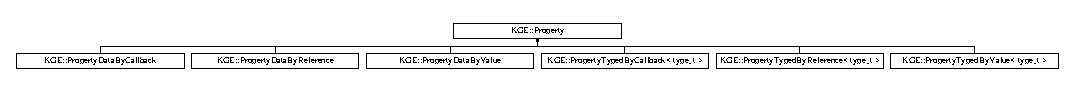
\includegraphics[height=0.699126cm]{class_k_g_e_1_1_property}
\end{center}
\end{figure}
\subsection*{Classes}
\begin{DoxyCompactItemize}
\item 
struct \hyperlink{struct_k_g_e_1_1_property_1_1_hasher}{Hasher}
\end{DoxyCompactItemize}
\subsection*{Public Member Functions}
\begin{DoxyCompactItemize}
\item 
\hypertarget{class_k_g_e_1_1_property_a9db7ae4492e59bd82fd9ed94c49653ee}{{\bfseries Property} (const \hyperlink{class_k_g_e_1_1_hash}{Hash} \&x\-Hash)}\label{class_k_g_e_1_1_property_a9db7ae4492e59bd82fd9ed94c49653ee}

\item 
\hypertarget{class_k_g_e_1_1_property_a2ede2e0955cacf076183e178219673c4}{virtual \hyperlink{class_k_g_e_1_1_data}{Data} {\bfseries Get\-Data} () const =0}\label{class_k_g_e_1_1_property_a2ede2e0955cacf076183e178219673c4}

\item 
\hypertarget{class_k_g_e_1_1_property_ae719405484bc7acb44d97cf781fe678d}{virtual void {\bfseries Set\-Data} (\hyperlink{class_k_g_e_1_1_data}{Data} x\-Data)=0}\label{class_k_g_e_1_1_property_ae719405484bc7acb44d97cf781fe678d}

\item 
\hypertarget{class_k_g_e_1_1_property_a45a44d831ad706b510c9f8a0c6ba205c}{virtual const \hyperlink{class_k_g_e_1_1_hash}{Hash} \& {\bfseries Get\-Hash} () const }\label{class_k_g_e_1_1_property_a45a44d831ad706b510c9f8a0c6ba205c}

\end{DoxyCompactItemize}
\subsection*{Protected Attributes}
\begin{DoxyCompactItemize}
\item 
\hypertarget{class_k_g_e_1_1_property_adc5c1288628b419954f24a754aa7662f}{\hyperlink{class_k_g_e_1_1_hash}{Hash} {\bfseries m\-\_\-x\-Hash}}\label{class_k_g_e_1_1_property_adc5c1288628b419954f24a754aa7662f}

\end{DoxyCompactItemize}


The documentation for this class was generated from the following file\-:\begin{DoxyCompactItemize}
\item 
C\-:/\-Users/\-Vit/\-Documents/\-Git\-Hub/\-K\-G\-E/\-K\-G\-E/\-Core/\-Class\-Capabilities/Properties.\-hpp\end{DoxyCompactItemize}

\hypertarget{class_k_g_e_1_1_property_data_by_callback}{\section{K\-G\-E\-:\-:Property\-Data\-By\-Callback Class Reference}
\label{class_k_g_e_1_1_property_data_by_callback}\index{K\-G\-E\-::\-Property\-Data\-By\-Callback@{K\-G\-E\-::\-Property\-Data\-By\-Callback}}
}
Inheritance diagram for K\-G\-E\-:\-:Property\-Data\-By\-Callback\-:\begin{figure}[H]
\begin{center}
\leavevmode
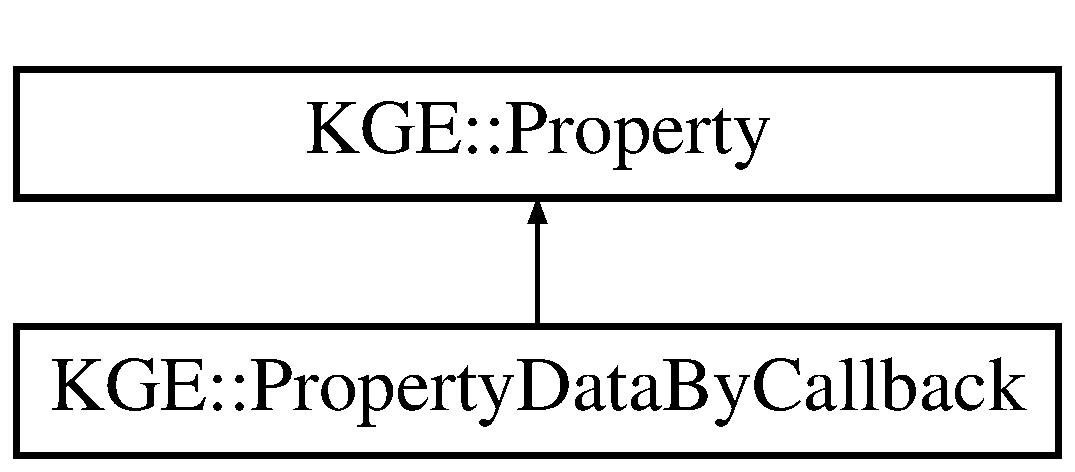
\includegraphics[height=2.000000cm]{class_k_g_e_1_1_property_data_by_callback}
\end{center}
\end{figure}
\subsection*{Public Member Functions}
\begin{DoxyCompactItemize}
\item 
\hypertarget{class_k_g_e_1_1_property_data_by_callback_a25300584870b77c3bd9fd7f4aa40358b}{{\bfseries Property\-Data\-By\-Callback} (const \hyperlink{class_k_g_e_1_1_hash}{Hash} \&x\-Hash, std\-::function$<$ \hyperlink{class_k_g_e_1_1_data}{Data}()$>$ \&x\-Get, std\-::function$<$ void(\hyperlink{class_k_g_e_1_1_data}{Data})$>$ \&x\-Set)}\label{class_k_g_e_1_1_property_data_by_callback_a25300584870b77c3bd9fd7f4aa40358b}

\item 
\hypertarget{class_k_g_e_1_1_property_data_by_callback_a4daa944a2121fc1ded5c7cee3006534a}{virtual \hyperlink{class_k_g_e_1_1_data}{Data} {\bfseries Get\-Data} () const }\label{class_k_g_e_1_1_property_data_by_callback_a4daa944a2121fc1ded5c7cee3006534a}

\item 
\hypertarget{class_k_g_e_1_1_property_data_by_callback_a7715f22f34f420601214d764e60f3c4a}{virtual void {\bfseries Set\-Data} (\hyperlink{class_k_g_e_1_1_data}{Data} x\-Data)}\label{class_k_g_e_1_1_property_data_by_callback_a7715f22f34f420601214d764e60f3c4a}

\end{DoxyCompactItemize}
\subsection*{Protected Attributes}
\begin{DoxyCompactItemize}
\item 
\hypertarget{class_k_g_e_1_1_property_data_by_callback_ac8208b2b303b7ffbf46cc30aba97d41a}{std\-::function$<$ \hyperlink{class_k_g_e_1_1_data}{Data}()$>$ \& {\bfseries m\-\_\-x\-Get}}\label{class_k_g_e_1_1_property_data_by_callback_ac8208b2b303b7ffbf46cc30aba97d41a}

\item 
\hypertarget{class_k_g_e_1_1_property_data_by_callback_ac3694eac39e19664078749e97fae4231}{std\-::function$<$ void(\hyperlink{class_k_g_e_1_1_data}{Data})$>$ \& {\bfseries m\-\_\-x\-Set}}\label{class_k_g_e_1_1_property_data_by_callback_ac3694eac39e19664078749e97fae4231}

\end{DoxyCompactItemize}


The documentation for this class was generated from the following file\-:\begin{DoxyCompactItemize}
\item 
C\-:/\-Users/\-Vit/\-Documents/\-Git\-Hub/\-K\-G\-E/\-K\-G\-E/\-Core/\-Class\-Capabilities/Properties.\-hpp\end{DoxyCompactItemize}

\hypertarget{class_k_g_e_1_1_property_data_by_reference}{\section{K\-G\-E\-:\-:Property\-Data\-By\-Reference Class Reference}
\label{class_k_g_e_1_1_property_data_by_reference}\index{K\-G\-E\-::\-Property\-Data\-By\-Reference@{K\-G\-E\-::\-Property\-Data\-By\-Reference}}
}
Inheritance diagram for K\-G\-E\-:\-:Property\-Data\-By\-Reference\-:\begin{figure}[H]
\begin{center}
\leavevmode
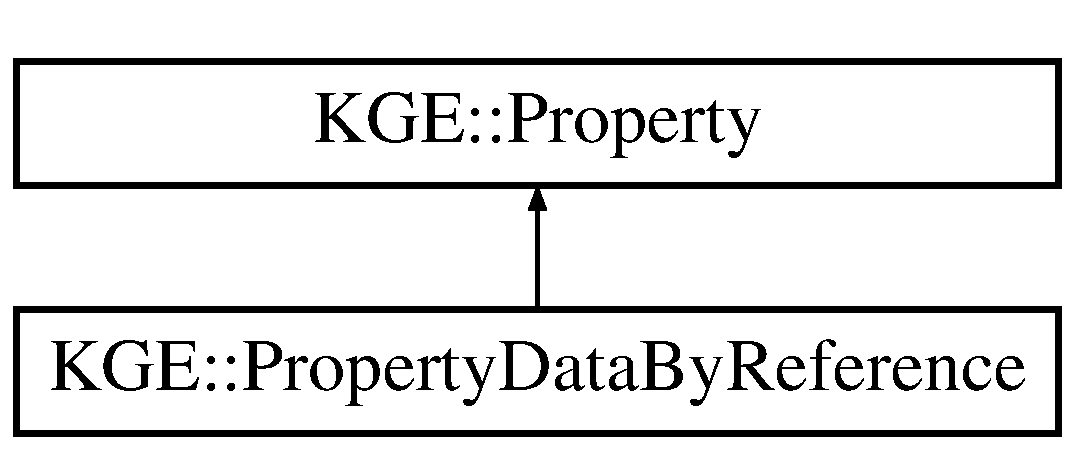
\includegraphics[height=2.000000cm]{class_k_g_e_1_1_property_data_by_reference}
\end{center}
\end{figure}
\subsection*{Public Member Functions}
\begin{DoxyCompactItemize}
\item 
\hypertarget{class_k_g_e_1_1_property_data_by_reference_af3df23a6fa9f76415da5786f82033ba7}{{\bfseries Property\-Data\-By\-Reference} (const \hyperlink{class_k_g_e_1_1_hash}{Hash} \&x\-Hash, \hyperlink{class_k_g_e_1_1_data}{Data} \&x\-Initial\-Data)}\label{class_k_g_e_1_1_property_data_by_reference_af3df23a6fa9f76415da5786f82033ba7}

\item 
\hypertarget{class_k_g_e_1_1_property_data_by_reference_affcbd041e32d676fcd062fb2e0556e7f}{virtual \hyperlink{class_k_g_e_1_1_data}{Data} {\bfseries Get\-Data} () const }\label{class_k_g_e_1_1_property_data_by_reference_affcbd041e32d676fcd062fb2e0556e7f}

\item 
\hypertarget{class_k_g_e_1_1_property_data_by_reference_aa06f1593adb338cd08bff28f9d8f3b6a}{virtual void {\bfseries Set\-Data} (\hyperlink{class_k_g_e_1_1_data}{Data} x\-Data)}\label{class_k_g_e_1_1_property_data_by_reference_aa06f1593adb338cd08bff28f9d8f3b6a}

\end{DoxyCompactItemize}
\subsection*{Protected Attributes}
\begin{DoxyCompactItemize}
\item 
\hypertarget{class_k_g_e_1_1_property_data_by_reference_a4f477343216bfd2de7272a51814d8ba6}{\hyperlink{class_k_g_e_1_1_data}{Data} \& {\bfseries m\-\_\-x\-Data}}\label{class_k_g_e_1_1_property_data_by_reference_a4f477343216bfd2de7272a51814d8ba6}

\end{DoxyCompactItemize}


The documentation for this class was generated from the following file\-:\begin{DoxyCompactItemize}
\item 
C\-:/\-Users/\-Vit/\-Documents/\-Git\-Hub/\-K\-G\-E/\-K\-G\-E/\-Core/\-Class\-Capabilities/Properties.\-hpp\end{DoxyCompactItemize}

\hypertarget{class_k_g_e_1_1_property_data_by_value}{\section{K\-G\-E\-:\-:Property\-Data\-By\-Value Class Reference}
\label{class_k_g_e_1_1_property_data_by_value}\index{K\-G\-E\-::\-Property\-Data\-By\-Value@{K\-G\-E\-::\-Property\-Data\-By\-Value}}
}
Inheritance diagram for K\-G\-E\-:\-:Property\-Data\-By\-Value\-:\begin{figure}[H]
\begin{center}
\leavevmode
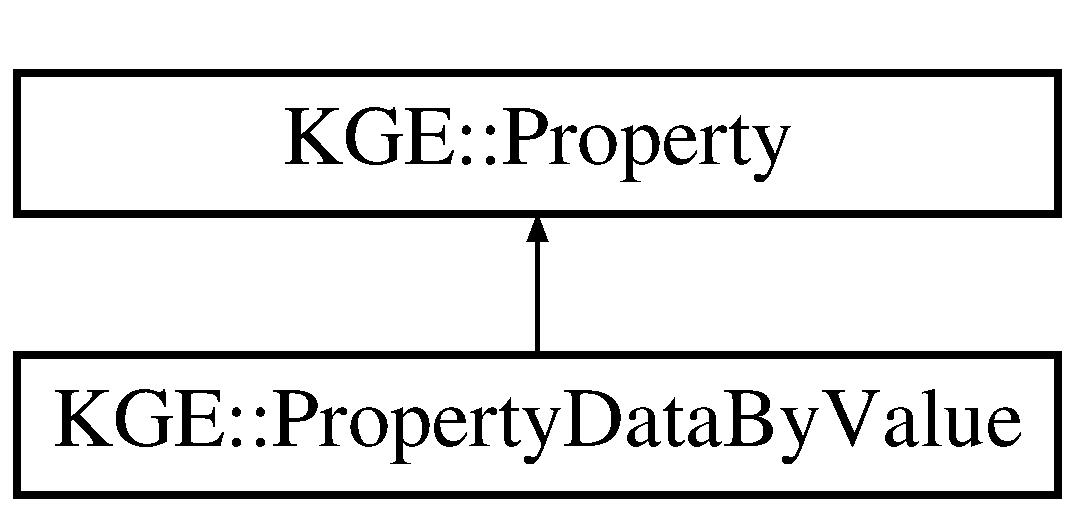
\includegraphics[height=2.000000cm]{class_k_g_e_1_1_property_data_by_value}
\end{center}
\end{figure}
\subsection*{Public Member Functions}
\begin{DoxyCompactItemize}
\item 
\hypertarget{class_k_g_e_1_1_property_data_by_value_ae6ab7e136376d75139ef09604b560a5e}{{\bfseries Property\-Data\-By\-Value} (const \hyperlink{class_k_g_e_1_1_hash}{Hash} \&x\-Hash, const \hyperlink{class_k_g_e_1_1_data}{Data} \&x\-Initial\-Data)}\label{class_k_g_e_1_1_property_data_by_value_ae6ab7e136376d75139ef09604b560a5e}

\item 
\hypertarget{class_k_g_e_1_1_property_data_by_value_a44144d25d9ec4131be7e78ffb6e4251d}{virtual \hyperlink{class_k_g_e_1_1_data}{Data} {\bfseries Get\-Data} () const }\label{class_k_g_e_1_1_property_data_by_value_a44144d25d9ec4131be7e78ffb6e4251d}

\item 
\hypertarget{class_k_g_e_1_1_property_data_by_value_abf7fed6702ea0ec5ae9ddc532b7b16f3}{virtual void {\bfseries Set\-Data} (\hyperlink{class_k_g_e_1_1_data}{Data} x\-Data)}\label{class_k_g_e_1_1_property_data_by_value_abf7fed6702ea0ec5ae9ddc532b7b16f3}

\end{DoxyCompactItemize}
\subsection*{Protected Attributes}
\begin{DoxyCompactItemize}
\item 
\hypertarget{class_k_g_e_1_1_property_data_by_value_ae72b8e5e5acada86cb5ad0c5b1ea007e}{\hyperlink{class_k_g_e_1_1_data}{Data} {\bfseries m\-\_\-x\-Data}}\label{class_k_g_e_1_1_property_data_by_value_ae72b8e5e5acada86cb5ad0c5b1ea007e}

\end{DoxyCompactItemize}


The documentation for this class was generated from the following file\-:\begin{DoxyCompactItemize}
\item 
C\-:/\-Users/\-Vit/\-Documents/\-Git\-Hub/\-K\-G\-E/\-K\-G\-E/\-Core/\-Class\-Capabilities/Properties.\-hpp\end{DoxyCompactItemize}

\hypertarget{class_k_g_e_1_1_property_typed_by_callback}{\section{K\-G\-E\-:\-:Property\-Typed\-By\-Callback$<$ type\-\_\-t $>$ Class Template Reference}
\label{class_k_g_e_1_1_property_typed_by_callback}\index{K\-G\-E\-::\-Property\-Typed\-By\-Callback$<$ type\-\_\-t $>$@{K\-G\-E\-::\-Property\-Typed\-By\-Callback$<$ type\-\_\-t $>$}}
}
Inheritance diagram for K\-G\-E\-:\-:Property\-Typed\-By\-Callback$<$ type\-\_\-t $>$\-:\begin{figure}[H]
\begin{center}
\leavevmode
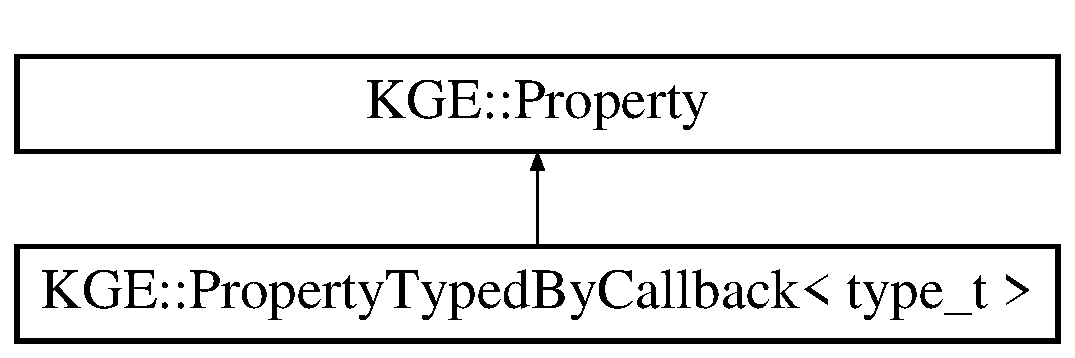
\includegraphics[height=2.000000cm]{class_k_g_e_1_1_property_typed_by_callback}
\end{center}
\end{figure}
\subsection*{Public Member Functions}
\begin{DoxyCompactItemize}
\item 
\hypertarget{class_k_g_e_1_1_property_typed_by_callback_aaf008232c13190a840d5f98919a1b36c}{{\bfseries Property\-Typed\-By\-Callback} (const \hyperlink{class_k_g_e_1_1_hash}{Hash} \&x\-Hash, std\-::function$<$ type\-\_\-t()$>$ \&x\-Get, std\-::function$<$ void(type\-\_\-t)$>$ \&x\-Set)}\label{class_k_g_e_1_1_property_typed_by_callback_aaf008232c13190a840d5f98919a1b36c}

\item 
\hypertarget{class_k_g_e_1_1_property_typed_by_callback_a1378c69b5eea301fa244bcf270a25301}{virtual \hyperlink{class_k_g_e_1_1_data}{Data} {\bfseries Get\-Data} () const }\label{class_k_g_e_1_1_property_typed_by_callback_a1378c69b5eea301fa244bcf270a25301}

\item 
\hypertarget{class_k_g_e_1_1_property_typed_by_callback_a089fcc45a9b1f44ccac1fd57a952edbb}{virtual void {\bfseries Set\-Data} (\hyperlink{class_k_g_e_1_1_data}{Data} x\-Data)}\label{class_k_g_e_1_1_property_typed_by_callback_a089fcc45a9b1f44ccac1fd57a952edbb}

\end{DoxyCompactItemize}
\subsection*{Protected Attributes}
\begin{DoxyCompactItemize}
\item 
\hypertarget{class_k_g_e_1_1_property_typed_by_callback_a6ad7424611873868ecfe2fabb060a348}{std\-::function$<$ type\-\_\-t()$>$ \& {\bfseries m\-\_\-x\-Get}}\label{class_k_g_e_1_1_property_typed_by_callback_a6ad7424611873868ecfe2fabb060a348}

\item 
\hypertarget{class_k_g_e_1_1_property_typed_by_callback_a8b2759750d6e55429e3802123332f0f5}{std\-::function$<$ void(type\-\_\-t)$>$ \& {\bfseries m\-\_\-x\-Set}}\label{class_k_g_e_1_1_property_typed_by_callback_a8b2759750d6e55429e3802123332f0f5}

\end{DoxyCompactItemize}


The documentation for this class was generated from the following file\-:\begin{DoxyCompactItemize}
\item 
C\-:/\-Users/\-Vit/\-Documents/\-Git\-Hub/\-K\-G\-E/\-K\-G\-E/\-Core/\-Class\-Capabilities/Properties.\-hpp\end{DoxyCompactItemize}

\hypertarget{class_k_g_e_1_1_property_typed_by_reference}{\section{K\-G\-E\-:\-:Property\-Typed\-By\-Reference$<$ type\-\_\-t $>$ Class Template Reference}
\label{class_k_g_e_1_1_property_typed_by_reference}\index{K\-G\-E\-::\-Property\-Typed\-By\-Reference$<$ type\-\_\-t $>$@{K\-G\-E\-::\-Property\-Typed\-By\-Reference$<$ type\-\_\-t $>$}}
}
Inheritance diagram for K\-G\-E\-:\-:Property\-Typed\-By\-Reference$<$ type\-\_\-t $>$\-:\begin{figure}[H]
\begin{center}
\leavevmode
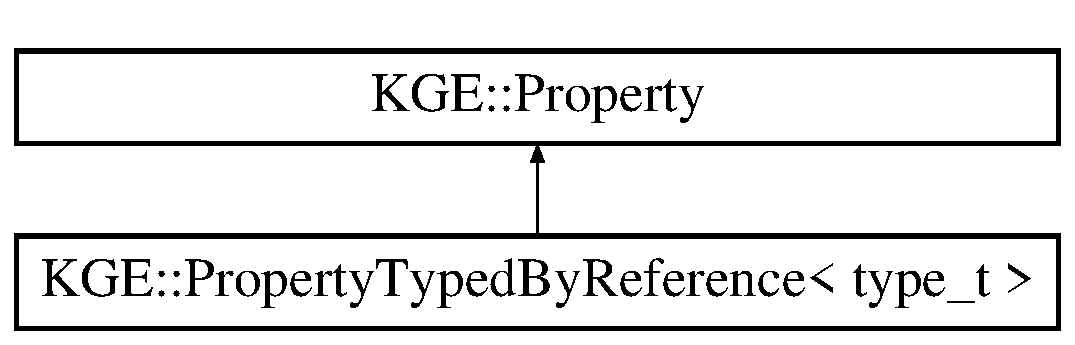
\includegraphics[height=2.000000cm]{class_k_g_e_1_1_property_typed_by_reference}
\end{center}
\end{figure}
\subsection*{Public Member Functions}
\begin{DoxyCompactItemize}
\item 
\hypertarget{class_k_g_e_1_1_property_typed_by_reference_aff31c400c785be13deea79b35be3f6ff}{{\bfseries Property\-Typed\-By\-Reference} (const \hyperlink{class_k_g_e_1_1_hash}{Hash} \&x\-Hash, type\-\_\-t x\-Initial\-Data)}\label{class_k_g_e_1_1_property_typed_by_reference_aff31c400c785be13deea79b35be3f6ff}

\item 
\hypertarget{class_k_g_e_1_1_property_typed_by_reference_a6ee5cda8c10bc9a4f82499f9f27b90c8}{virtual \hyperlink{class_k_g_e_1_1_data}{Data} {\bfseries Get\-Data} () const }\label{class_k_g_e_1_1_property_typed_by_reference_a6ee5cda8c10bc9a4f82499f9f27b90c8}

\item 
\hypertarget{class_k_g_e_1_1_property_typed_by_reference_af74dd297ad8db9d3e3e75d0aef82dd29}{virtual void {\bfseries Set\-Data} (\hyperlink{class_k_g_e_1_1_data}{Data} x\-Data)}\label{class_k_g_e_1_1_property_typed_by_reference_af74dd297ad8db9d3e3e75d0aef82dd29}

\end{DoxyCompactItemize}
\subsection*{Protected Attributes}
\begin{DoxyCompactItemize}
\item 
\hypertarget{class_k_g_e_1_1_property_typed_by_reference_a1b002909b55b67d036ef6ccc4afb4f84}{type\-\_\-t \& {\bfseries m\-\_\-x\-Data}}\label{class_k_g_e_1_1_property_typed_by_reference_a1b002909b55b67d036ef6ccc4afb4f84}

\end{DoxyCompactItemize}


The documentation for this class was generated from the following file\-:\begin{DoxyCompactItemize}
\item 
C\-:/\-Users/\-Vit/\-Documents/\-Git\-Hub/\-K\-G\-E/\-K\-G\-E/\-Core/\-Class\-Capabilities/Properties.\-hpp\end{DoxyCompactItemize}

\hypertarget{class_k_g_e_1_1_property_typed_by_value}{\section{K\-G\-E\-:\-:Property\-Typed\-By\-Value$<$ type\-\_\-t $>$ Class Template Reference}
\label{class_k_g_e_1_1_property_typed_by_value}\index{K\-G\-E\-::\-Property\-Typed\-By\-Value$<$ type\-\_\-t $>$@{K\-G\-E\-::\-Property\-Typed\-By\-Value$<$ type\-\_\-t $>$}}
}
Inheritance diagram for K\-G\-E\-:\-:Property\-Typed\-By\-Value$<$ type\-\_\-t $>$\-:\begin{figure}[H]
\begin{center}
\leavevmode
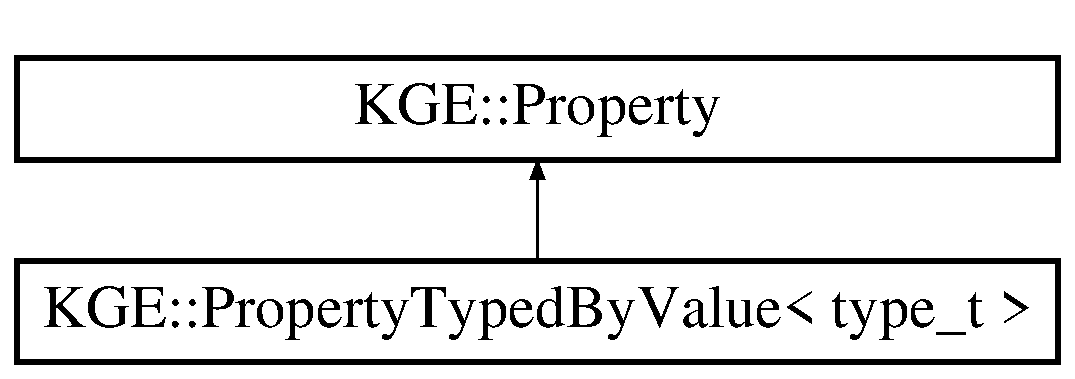
\includegraphics[height=2.000000cm]{class_k_g_e_1_1_property_typed_by_value}
\end{center}
\end{figure}
\subsection*{Public Member Functions}
\begin{DoxyCompactItemize}
\item 
\hypertarget{class_k_g_e_1_1_property_typed_by_value_a0a024431a770645c7b6379f2bb943b80}{{\bfseries Property\-Typed\-By\-Value} (const \hyperlink{class_k_g_e_1_1_hash}{Hash} \&x\-Hash, type\-\_\-t x\-Initial\-Data)}\label{class_k_g_e_1_1_property_typed_by_value_a0a024431a770645c7b6379f2bb943b80}

\item 
\hypertarget{class_k_g_e_1_1_property_typed_by_value_af2fcefa3196c25cb747a0fbf66fceab1}{virtual \hyperlink{class_k_g_e_1_1_data}{Data} {\bfseries Get\-Data} () const }\label{class_k_g_e_1_1_property_typed_by_value_af2fcefa3196c25cb747a0fbf66fceab1}

\item 
\hypertarget{class_k_g_e_1_1_property_typed_by_value_a08d0237f52822663b9252818967fca77}{virtual void {\bfseries Set\-Data} (\hyperlink{class_k_g_e_1_1_data}{Data} x\-Data)}\label{class_k_g_e_1_1_property_typed_by_value_a08d0237f52822663b9252818967fca77}

\end{DoxyCompactItemize}
\subsection*{Protected Attributes}
\begin{DoxyCompactItemize}
\item 
\hypertarget{class_k_g_e_1_1_property_typed_by_value_a179924a3f3b1acf9c984f05ded2791bb}{type\-\_\-t {\bfseries m\-\_\-x\-Data}}\label{class_k_g_e_1_1_property_typed_by_value_a179924a3f3b1acf9c984f05ded2791bb}

\end{DoxyCompactItemize}


The documentation for this class was generated from the following file\-:\begin{DoxyCompactItemize}
\item 
C\-:/\-Users/\-Vit/\-Documents/\-Git\-Hub/\-K\-G\-E/\-K\-G\-E/\-Core/\-Class\-Capabilities/Properties.\-hpp\end{DoxyCompactItemize}

\hypertarget{class_k_g_e_1_1_sprite}{\section{K\-G\-E\-:\-:Sprite Class Reference}
\label{class_k_g_e_1_1_sprite}\index{K\-G\-E\-::\-Sprite@{K\-G\-E\-::\-Sprite}}
}


The documentation for this class was generated from the following file\-:\begin{DoxyCompactItemize}
\item 
C\-:/\-Users/\-Vit/\-Documents/\-Git\-Hub/\-K\-G\-E/\-K\-G\-E/\-Core/\-Graphics/Sprite.\-hpp\end{DoxyCompactItemize}

\hypertarget{class_k_g_e_1_1_texture_manager}{\section{K\-G\-E\-:\-:Texture\-Manager Class Reference}
\label{class_k_g_e_1_1_texture_manager}\index{K\-G\-E\-::\-Texture\-Manager@{K\-G\-E\-::\-Texture\-Manager}}
}
\subsection*{Public Member Functions}
\begin{DoxyCompactItemize}
\item 
\hypertarget{class_k_g_e_1_1_texture_manager_a7d740cf85dc9df88e3c6853d35d5c753}{sf\-::\-Texture $\ast$ {\bfseries Load\-Texture} (const std\-::string \&sz\-File\-Name)}\label{class_k_g_e_1_1_texture_manager_a7d740cf85dc9df88e3c6853d35d5c753}

\item 
\hypertarget{class_k_g_e_1_1_texture_manager_a1abdbc9f8ef1fe47c0bb7513a822f3fa}{sf\-::\-Texture $\ast$ {\bfseries Load\-Texture\-With\-Alias} (const std\-::string \&sz\-File\-Name, const \hyperlink{class_k_g_e_1_1_hash}{Hash} \&x\-Alias)}\label{class_k_g_e_1_1_texture_manager_a1abdbc9f8ef1fe47c0bb7513a822f3fa}

\item 
\hypertarget{class_k_g_e_1_1_texture_manager_a4ea7f58cfcc584a0f02f992bae5761df}{sf\-::\-Texture $\ast$ {\bfseries Get\-Texture} (const \hyperlink{class_k_g_e_1_1_hash}{Hash} \&x\-Hash)}\label{class_k_g_e_1_1_texture_manager_a4ea7f58cfcc584a0f02f992bae5761df}

\item 
\hypertarget{class_k_g_e_1_1_texture_manager_a59541f59c443cb7590d890fbfcadcce4}{void {\bfseries Release\-Texture} (const \hyperlink{class_k_g_e_1_1_hash}{Hash} \&x\-Hash)}\label{class_k_g_e_1_1_texture_manager_a59541f59c443cb7590d890fbfcadcce4}

\item 
\hypertarget{class_k_g_e_1_1_texture_manager_a3b556b077b352cab09b33f3e35f29ee9}{void {\bfseries Release\-Texture} (sf\-::\-Texture $\ast$px\-Texture)}\label{class_k_g_e_1_1_texture_manager_a3b556b077b352cab09b33f3e35f29ee9}

\end{DoxyCompactItemize}
\subsection*{Static Public Member Functions}
\begin{DoxyCompactItemize}
\item 
\hypertarget{class_k_g_e_1_1_texture_manager_a578aaeb0808f1f42299057cae1f6c3d1}{static \hyperlink{class_k_g_e_1_1_texture_manager}{Texture\-Manager} \& {\bfseries Get} ()}\label{class_k_g_e_1_1_texture_manager_a578aaeb0808f1f42299057cae1f6c3d1}

\end{DoxyCompactItemize}
\subsection*{Protected Attributes}
\begin{DoxyCompactItemize}
\item 
\hypertarget{class_k_g_e_1_1_texture_manager_a802c199bf3be354d1ee2e1cdfb836c32}{texturecollection\-\_\-t {\bfseries m\-\_\-x\-Texture\-List}}\label{class_k_g_e_1_1_texture_manager_a802c199bf3be354d1ee2e1cdfb836c32}

\end{DoxyCompactItemize}


The documentation for this class was generated from the following files\-:\begin{DoxyCompactItemize}
\item 
C\-:/\-Users/\-Vit/\-Documents/\-Git\-Hub/\-K\-G\-E/\-K\-G\-E/\-Core/\-Resources/Texture\-Manager.\-hpp\item 
C\-:/\-Users/\-Vit/\-Documents/\-Git\-Hub/\-K\-G\-E/\-K\-G\-E/\-Core/\-Resources/Texture\-Manager.\-cpp\end{DoxyCompactItemize}

\hypertarget{class_k_g_e_1_1_t_u_i_d}{\section{K\-G\-E\-:\-:T\-U\-I\-D$<$ T\-Object $>$ Class Template Reference}
\label{class_k_g_e_1_1_t_u_i_d}\index{K\-G\-E\-::\-T\-U\-I\-D$<$ T\-Object $>$@{K\-G\-E\-::\-T\-U\-I\-D$<$ T\-Object $>$}}
}
\subsection*{Classes}
\begin{DoxyCompactItemize}
\item 
class \hyperlink{class_k_g_e_1_1_t_u_i_d_1_1_cached_reference}{Cached\-Reference}
\item 
struct \hyperlink{struct_k_g_e_1_1_t_u_i_d_1_1_hasher}{Hasher}
\item 
struct \hyperlink{struct_k_g_e_1_1_t_u_i_d_1_1_manager}{Manager}
\end{DoxyCompactItemize}
\subsection*{Public Member Functions}
\begin{DoxyCompactItemize}
\item 
\hypertarget{class_k_g_e_1_1_t_u_i_d_abf6fc57819dc1f875ab707dc505e9019}{{\bfseries T\-U\-I\-D} (T\-Object \&x\-Target)}\label{class_k_g_e_1_1_t_u_i_d_abf6fc57819dc1f875ab707dc505e9019}

\item 
\hypertarget{class_k_g_e_1_1_t_u_i_d_a62f3668bcd3e59b63d1ae7b5767d28bf}{\hyperlink{class_k_g_e_1_1_t_u_i_d_1_1_cached_reference}{Cached\-Reference} {\bfseries Get\-Cached\-Reference} () const }\label{class_k_g_e_1_1_t_u_i_d_a62f3668bcd3e59b63d1ae7b5767d28bf}

\item 
\hypertarget{class_k_g_e_1_1_t_u_i_d_a176685d0697073bb1c884ecff5610cd1}{void {\bfseries Invalidate} ()}\label{class_k_g_e_1_1_t_u_i_d_a176685d0697073bb1c884ecff5610cd1}

\item 
\hypertarget{class_k_g_e_1_1_t_u_i_d_abb94f7ce3ac1b06030d59982ef57d1e4}{bool {\bfseries Is\-Invalid} () const }\label{class_k_g_e_1_1_t_u_i_d_abb94f7ce3ac1b06030d59982ef57d1e4}

\item 
\hypertarget{class_k_g_e_1_1_t_u_i_d_a991ec67886d4010209a8b8284260d7f7}{void {\bfseries operator=} (const \hyperlink{class_k_g_e_1_1_t_u_i_d}{T\-U\-I\-D} \&b)}\label{class_k_g_e_1_1_t_u_i_d_a991ec67886d4010209a8b8284260d7f7}

\item 
\hypertarget{class_k_g_e_1_1_t_u_i_d_af87d643733c348eb22122847f3b2c974}{bool {\bfseries operator==} (const \hyperlink{class_k_g_e_1_1_t_u_i_d}{T\-U\-I\-D} \&b) const }\label{class_k_g_e_1_1_t_u_i_d_af87d643733c348eb22122847f3b2c974}

\item 
\hypertarget{class_k_g_e_1_1_t_u_i_d_a716b9cde910775c2d0d40f963f285f1f}{bool {\bfseries operator!=} (const \hyperlink{class_k_g_e_1_1_t_u_i_d}{T\-U\-I\-D} \&b) const }\label{class_k_g_e_1_1_t_u_i_d_a716b9cde910775c2d0d40f963f285f1f}

\item 
\hypertarget{class_k_g_e_1_1_t_u_i_d_a10d364e97335e4d3ba4a2578c6dbbb39}{bool {\bfseries operator$<$} (const \hyperlink{class_k_g_e_1_1_t_u_i_d}{T\-U\-I\-D} \&b) const }\label{class_k_g_e_1_1_t_u_i_d_a10d364e97335e4d3ba4a2578c6dbbb39}

\end{DoxyCompactItemize}
\subsection*{Static Public Attributes}
\begin{DoxyCompactItemize}
\item 
\hypertarget{class_k_g_e_1_1_t_u_i_d_a21cb15152251a6ec71f1d77bb9c55b51}{static const unsigned int {\bfseries U\-N\-S\-E\-T} = 0}\label{class_k_g_e_1_1_t_u_i_d_a21cb15152251a6ec71f1d77bb9c55b51}

\end{DoxyCompactItemize}
\subsection*{Protected Member Functions}
\begin{DoxyCompactItemize}
\item 
\hypertarget{class_k_g_e_1_1_t_u_i_d_acc7f7cd5d011a6bd1c14384f77beb4a8}{{\bfseries T\-U\-I\-D} (const \hyperlink{class_k_g_e_1_1_t_u_i_d}{T\-U\-I\-D} \&x\-Copy)}\label{class_k_g_e_1_1_t_u_i_d_acc7f7cd5d011a6bd1c14384f77beb4a8}

\end{DoxyCompactItemize}
\subsection*{Static Protected Member Functions}
\begin{DoxyCompactItemize}
\item 
\hypertarget{class_k_g_e_1_1_t_u_i_d_a6b33cdc8bcb9290470c7aed787e39771}{static \hyperlink{struct_k_g_e_1_1_t_u_i_d_1_1_manager}{Manager} \& {\bfseries Get\-Manager} ()}\label{class_k_g_e_1_1_t_u_i_d_a6b33cdc8bcb9290470c7aed787e39771}

\end{DoxyCompactItemize}
\subsection*{Protected Attributes}
\begin{DoxyCompactItemize}
\item 
\hypertarget{class_k_g_e_1_1_t_u_i_d_a64cbab98483640428c5c588128edf2f9}{T\-Object \& {\bfseries m\-\_\-x\-Target}}\label{class_k_g_e_1_1_t_u_i_d_a64cbab98483640428c5c588128edf2f9}

\item 
\hypertarget{class_k_g_e_1_1_t_u_i_d_a26c37e58a36e76791d69dc65a139f194}{u\-\_\-int {\bfseries m\-\_\-u\-T\-U\-I\-D}}\label{class_k_g_e_1_1_t_u_i_d_a26c37e58a36e76791d69dc65a139f194}

\end{DoxyCompactItemize}
\subsection*{Friends}
\begin{DoxyCompactItemize}
\item 
\hypertarget{class_k_g_e_1_1_t_u_i_d_a1fd6b9bc3f72bb2b64e602de3982929d}{struct {\bfseries Manager}}\label{class_k_g_e_1_1_t_u_i_d_a1fd6b9bc3f72bb2b64e602de3982929d}

\item 
\hypertarget{class_k_g_e_1_1_t_u_i_d_abae691ad248b86e85d4bc04709d2f39e}{class {\bfseries Cached\-Reference}}\label{class_k_g_e_1_1_t_u_i_d_abae691ad248b86e85d4bc04709d2f39e}

\end{DoxyCompactItemize}


The documentation for this class was generated from the following file\-:\begin{DoxyCompactItemize}
\item 
C\-:/\-Users/\-Vit/\-Documents/\-Git\-Hub/\-K\-G\-E/\-K\-G\-E/\-Core/\-Data/T\-U\-I\-D.\-hpp\end{DoxyCompactItemize}

\hypertarget{struct_k_g_e_1_1_vec2f}{\section{K\-G\-E\-:\-:Vec2f Struct Reference}
\label{struct_k_g_e_1_1_vec2f}\index{K\-G\-E\-::\-Vec2f@{K\-G\-E\-::\-Vec2f}}
}
\subsection*{Public Member Functions}
\begin{DoxyCompactItemize}
\item 
\hypertarget{struct_k_g_e_1_1_vec2f_a295c1fd5d8a1206e189eb56180fa2720}{{\bfseries Vec2f} (float f\-X, float f\-Y)}\label{struct_k_g_e_1_1_vec2f_a295c1fd5d8a1206e189eb56180fa2720}

\item 
\hypertarget{struct_k_g_e_1_1_vec2f_a79a4eb6d91c80cb3d692845f9abb5918}{{\bfseries Vec2f} (const \hyperlink{struct_k_g_e_1_1_vec2f}{Vec2f} \&x\-Copy)}\label{struct_k_g_e_1_1_vec2f_a79a4eb6d91c80cb3d692845f9abb5918}

\item 
\hypertarget{struct_k_g_e_1_1_vec2f_a62bdfd01997b7c2175cc23804e468743}{float {\bfseries Magnitude} () const }\label{struct_k_g_e_1_1_vec2f_a62bdfd01997b7c2175cc23804e468743}

\item 
\hypertarget{struct_k_g_e_1_1_vec2f_a704881b909c4a6f32926db57acc0c063}{float {\bfseries Magnitude\-Sq} () const }\label{struct_k_g_e_1_1_vec2f_a704881b909c4a6f32926db57acc0c063}

\item 
\hypertarget{struct_k_g_e_1_1_vec2f_ae7ab2bd76a369c8293a419fc8983c5c4}{float {\bfseries Normalise} ()}\label{struct_k_g_e_1_1_vec2f_ae7ab2bd76a369c8293a419fc8983c5c4}

\item 
\hypertarget{struct_k_g_e_1_1_vec2f_a1eccb56f05d77248d59ed17684b7e73b}{\hyperlink{struct_k_g_e_1_1_vec2f}{Vec2f} {\bfseries operator$\ast$} (float f\-R\-H\-S) const }\label{struct_k_g_e_1_1_vec2f_a1eccb56f05d77248d59ed17684b7e73b}

\item 
\hypertarget{struct_k_g_e_1_1_vec2f_adeb44e2cba0f80008351ebcbd4fc2b82}{void {\bfseries operator$\ast$=} (float f\-R\-H\-S)}\label{struct_k_g_e_1_1_vec2f_adeb44e2cba0f80008351ebcbd4fc2b82}

\item 
\hypertarget{struct_k_g_e_1_1_vec2f_a0035decd7d54ed75f96bb08d56371acc}{bool {\bfseries operator==} (const \hyperlink{struct_k_g_e_1_1_vec2f}{Vec2f} \&x\-R\-H\-S) const }\label{struct_k_g_e_1_1_vec2f_a0035decd7d54ed75f96bb08d56371acc}

\item 
\hypertarget{struct_k_g_e_1_1_vec2f_abe9aa2d7614f797fbc98a315f7f7c262}{bool {\bfseries operator!=} (const \hyperlink{struct_k_g_e_1_1_vec2f}{Vec2f} \&x\-R\-H\-S) const }\label{struct_k_g_e_1_1_vec2f_abe9aa2d7614f797fbc98a315f7f7c262}

\item 
\hypertarget{struct_k_g_e_1_1_vec2f_a632f6b063debf7935a798e05c14984eb}{void {\bfseries operator+=} (const \hyperlink{struct_k_g_e_1_1_vec2f}{Vec2f} \&x\-R\-H\-S)}\label{struct_k_g_e_1_1_vec2f_a632f6b063debf7935a798e05c14984eb}

\item 
\hypertarget{struct_k_g_e_1_1_vec2f_a76d6dce3a9a27be5d5bc422af3568127}{void {\bfseries operator-\/=} (const \hyperlink{struct_k_g_e_1_1_vec2f}{Vec2f} \&x\-R\-H\-S)}\label{struct_k_g_e_1_1_vec2f_a76d6dce3a9a27be5d5bc422af3568127}

\item 
\hypertarget{struct_k_g_e_1_1_vec2f_a7bac4e9fccb38c4d9d3530b725df12e3}{\hyperlink{struct_k_g_e_1_1_vec2f}{Vec2f} {\bfseries operator+} (const \hyperlink{struct_k_g_e_1_1_vec2f}{Vec2f} \&x\-R\-H\-S) const }\label{struct_k_g_e_1_1_vec2f_a7bac4e9fccb38c4d9d3530b725df12e3}

\item 
\hypertarget{struct_k_g_e_1_1_vec2f_a781ea1f86fa2bb67a216aed98c825a19}{\hyperlink{struct_k_g_e_1_1_vec2f}{Vec2f} {\bfseries operator-\/} (const \hyperlink{struct_k_g_e_1_1_vec2f}{Vec2f} \&x\-R\-H\-S) const }\label{struct_k_g_e_1_1_vec2f_a781ea1f86fa2bb67a216aed98c825a19}

\item 
\hypertarget{struct_k_g_e_1_1_vec2f_a3ffb1b191ee357bf1819e3bf33184cdd}{float {\bfseries To\-Angle} () const }\label{struct_k_g_e_1_1_vec2f_a3ffb1b191ee357bf1819e3bf33184cdd}

\item 
\hypertarget{struct_k_g_e_1_1_vec2f_a914c2b85b3fd4de7f5b551a2abe04fa1}{void {\bfseries Set\-From\-Angle} (float f\-Angle, float f\-Magnitude=1.\-0f)}\label{struct_k_g_e_1_1_vec2f_a914c2b85b3fd4de7f5b551a2abe04fa1}

\item 
\hypertarget{struct_k_g_e_1_1_vec2f_ae488e5bc056d7fbd4ddc66ad29919045}{void {\bfseries Rotate\-By} (float f\-Angle)}\label{struct_k_g_e_1_1_vec2f_ae488e5bc056d7fbd4ddc66ad29919045}

\item 
\hypertarget{struct_k_g_e_1_1_vec2f_a2d4d63080909bf0ab73c9e8c401f410b}{const sf\-::\-Vector2f \& {\bfseries As\-S\-F\-Vec2f} () const }\label{struct_k_g_e_1_1_vec2f_a2d4d63080909bf0ab73c9e8c401f410b}

\item 
\hypertarget{struct_k_g_e_1_1_vec2f_a50b74040f634a3d78c19a532bd6af796}{sf\-::\-Vector2f \& {\bfseries As\-S\-F\-Vec2f} ()}\label{struct_k_g_e_1_1_vec2f_a50b74040f634a3d78c19a532bd6af796}

\item 
\hypertarget{struct_k_g_e_1_1_vec2f_a4a1c611efeb73173cd9fd9105acfeead}{const b2\-Vec2 \& {\bfseries As\-B2\-Vec2} () const }\label{struct_k_g_e_1_1_vec2f_a4a1c611efeb73173cd9fd9105acfeead}

\item 
\hypertarget{struct_k_g_e_1_1_vec2f_aec2d0ce1bb97c6e86972776b426a0d13}{b2\-Vec2 \& {\bfseries As\-B2\-Vec2} ()}\label{struct_k_g_e_1_1_vec2f_aec2d0ce1bb97c6e86972776b426a0d13}

\item 
\hypertarget{struct_k_g_e_1_1_vec2f_a9a2a8f7ff15e80cb9223ce04b0479915}{void {\bfseries Read\-From\-String} (const char $\ast$sz\-Input)}\label{struct_k_g_e_1_1_vec2f_a9a2a8f7ff15e80cb9223ce04b0479915}

\end{DoxyCompactItemize}
\subsection*{Static Public Member Functions}
\begin{DoxyCompactItemize}
\item 
\hypertarget{struct_k_g_e_1_1_vec2f_a37839e755faa101c9403c1f3858bc10c}{static \hyperlink{struct_k_g_e_1_1_vec2f}{Vec2f} {\bfseries Create\-From\-Angle} (float f\-Angle, float f\-Magnitude=1.\-0f)}\label{struct_k_g_e_1_1_vec2f_a37839e755faa101c9403c1f3858bc10c}

\item 
\hypertarget{struct_k_g_e_1_1_vec2f_aade5b26b17c1bbb68e2c74b1b454fb19}{static \hyperlink{struct_k_g_e_1_1_vec2f}{Vec2f} {\bfseries Rotate\-By} (\hyperlink{struct_k_g_e_1_1_vec2f}{Vec2f} x\-Input, float f\-Angle)}\label{struct_k_g_e_1_1_vec2f_aade5b26b17c1bbb68e2c74b1b454fb19}

\end{DoxyCompactItemize}
\subsection*{Public Attributes}
\begin{DoxyCompactItemize}
\item 
\hypertarget{struct_k_g_e_1_1_vec2f_a31c19904eceee952d34af9f8bf71185c}{float {\bfseries X}}\label{struct_k_g_e_1_1_vec2f_a31c19904eceee952d34af9f8bf71185c}

\item 
\hypertarget{struct_k_g_e_1_1_vec2f_a19f6b7acba72df3e1fca642ed68a80df}{float {\bfseries Y}}\label{struct_k_g_e_1_1_vec2f_a19f6b7acba72df3e1fca642ed68a80df}

\end{DoxyCompactItemize}


The documentation for this struct was generated from the following files\-:\begin{DoxyCompactItemize}
\item 
C\-:/\-Users/\-Vit/\-Documents/\-Git\-Hub/\-K\-G\-E/\-K\-G\-E/\-Core/\-Maths/Vec2f.\-hpp\item 
C\-:/\-Users/\-Vit/\-Documents/\-Git\-Hub/\-K\-G\-E/\-K\-G\-E/\-Core/\-Maths/Vec2f.\-cpp\end{DoxyCompactItemize}

\hypertarget{class_k_g_e_1_1_x_m_l_attribute_handler}{\section{K\-G\-E\-:\-:X\-M\-L\-Attribute\-Handler$<$ parent\-\_\-t $>$ Class Template Reference}
\label{class_k_g_e_1_1_x_m_l_attribute_handler}\index{K\-G\-E\-::\-X\-M\-L\-Attribute\-Handler$<$ parent\-\_\-t $>$@{K\-G\-E\-::\-X\-M\-L\-Attribute\-Handler$<$ parent\-\_\-t $>$}}
}
\subsection*{Public Types}
\begin{DoxyCompactItemize}
\item 
\hypertarget{class_k_g_e_1_1_x_m_l_attribute_handler_aac0ba9461ecd0f95b64b3de8987a17d1}{typedef void(parent\-\_\-t\-::$\ast$ {\bfseries Attribute\-Callback\-Fn\-Ptr} )(xml\-\_\-attribute$<$ char $>$ \&)}\label{class_k_g_e_1_1_x_m_l_attribute_handler_aac0ba9461ecd0f95b64b3de8987a17d1}

\end{DoxyCompactItemize}
\subsection*{Public Member Functions}
\begin{DoxyCompactItemize}
\item 
\hypertarget{class_k_g_e_1_1_x_m_l_attribute_handler_ab0d6fefb953c5b400f551f3c968b474b}{{\bfseries X\-M\-L\-Attribute\-Handler} (\hyperlink{class_k_g_e_1_1_hash}{Hash} x\-Name\-Hash, Attribute\-Callback\-Fn\-Ptr px\-Callback)}\label{class_k_g_e_1_1_x_m_l_attribute_handler_ab0d6fefb953c5b400f551f3c968b474b}

\item 
\hypertarget{class_k_g_e_1_1_x_m_l_attribute_handler_a73b9328398e4682e6bd927673ab94b6f}{void {\bfseries Process} (xml\-\_\-attribute$<$ char $>$ \&x\-Attribute, parent\-\_\-t $\ast$px\-This) const }\label{class_k_g_e_1_1_x_m_l_attribute_handler_a73b9328398e4682e6bd927673ab94b6f}

\end{DoxyCompactItemize}
\subsection*{Protected Attributes}
\begin{DoxyCompactItemize}
\item 
\hypertarget{class_k_g_e_1_1_x_m_l_attribute_handler_a3a2e1be1a6a09096dfac40410c05c802}{Attribute\-Callback\-Fn\-Ptr {\bfseries m\-\_\-px\-Callback}}\label{class_k_g_e_1_1_x_m_l_attribute_handler_a3a2e1be1a6a09096dfac40410c05c802}

\end{DoxyCompactItemize}


The documentation for this class was generated from the following file\-:\begin{DoxyCompactItemize}
\item 
C\-:/\-Users/\-Vit/\-Documents/\-Git\-Hub/\-K\-G\-E/\-K\-G\-E/\-Core/\-Class\-Capabilities/X\-M\-L\-Parser.\-hpp\end{DoxyCompactItemize}

\hypertarget{class_k_g_e_1_1_x_m_l_child_handler}{\section{K\-G\-E\-:\-:X\-M\-L\-Child\-Handler$<$ parent\-\_\-t $>$ Class Template Reference}
\label{class_k_g_e_1_1_x_m_l_child_handler}\index{K\-G\-E\-::\-X\-M\-L\-Child\-Handler$<$ parent\-\_\-t $>$@{K\-G\-E\-::\-X\-M\-L\-Child\-Handler$<$ parent\-\_\-t $>$}}
}
\subsection*{Public Types}
\begin{DoxyCompactItemize}
\item 
\hypertarget{class_k_g_e_1_1_x_m_l_child_handler_a0ca5aedec77909e6a11f6391e920bb85}{typedef void(parent\-\_\-t\-::$\ast$ {\bfseries Node\-Callback\-Fn\-Ptr} )(xml\-\_\-node$<$ char $>$ \&)}\label{class_k_g_e_1_1_x_m_l_child_handler_a0ca5aedec77909e6a11f6391e920bb85}

\end{DoxyCompactItemize}
\subsection*{Public Member Functions}
\begin{DoxyCompactItemize}
\item 
\hypertarget{class_k_g_e_1_1_x_m_l_child_handler_aa6334139a13ae6f5b9f48fc3e695849f}{{\bfseries X\-M\-L\-Child\-Handler} (\hyperlink{class_k_g_e_1_1_hash}{Hash} x\-Name\-Hash, Node\-Callback\-Fn\-Ptr px\-Callback)}\label{class_k_g_e_1_1_x_m_l_child_handler_aa6334139a13ae6f5b9f48fc3e695849f}

\item 
\hypertarget{class_k_g_e_1_1_x_m_l_child_handler_ad0b708157a391d15b9027c951ce36c92}{void {\bfseries Process} (xml\-\_\-node$<$ char $>$ \&x\-Node, parent\-\_\-t $\ast$px\-This) const }\label{class_k_g_e_1_1_x_m_l_child_handler_ad0b708157a391d15b9027c951ce36c92}

\end{DoxyCompactItemize}
\subsection*{Protected Attributes}
\begin{DoxyCompactItemize}
\item 
\hypertarget{class_k_g_e_1_1_x_m_l_child_handler_a8267c91e2b7b669c5aefb37383047472}{Node\-Callback\-Fn\-Ptr {\bfseries m\-\_\-px\-Callback}}\label{class_k_g_e_1_1_x_m_l_child_handler_a8267c91e2b7b669c5aefb37383047472}

\end{DoxyCompactItemize}


The documentation for this class was generated from the following file\-:\begin{DoxyCompactItemize}
\item 
C\-:/\-Users/\-Vit/\-Documents/\-Git\-Hub/\-K\-G\-E/\-K\-G\-E/\-Core/\-Class\-Capabilities/X\-M\-L\-Parser.\-hpp\end{DoxyCompactItemize}

\hypertarget{class_k_g_e_1_1_x_m_l_helpers}{\section{K\-G\-E\-:\-:X\-M\-L\-Helpers Class Reference}
\label{class_k_g_e_1_1_x_m_l_helpers}\index{K\-G\-E\-::\-X\-M\-L\-Helpers@{K\-G\-E\-::\-X\-M\-L\-Helpers}}
}
\subsection*{Static Public Member Functions}
\begin{DoxyCompactItemize}
\item 
\hypertarget{class_k_g_e_1_1_x_m_l_helpers_a995e42ae1d73fdd7b811fae44b1da23d}{static const char $\ast$ {\bfseries Get\-Attribute\-Value} (xml\-\_\-node$<$ char $>$ \&x\-Object, const char $\ast$sz\-Attribute)}\label{class_k_g_e_1_1_x_m_l_helpers_a995e42ae1d73fdd7b811fae44b1da23d}

\end{DoxyCompactItemize}


The documentation for this class was generated from the following file\-:\begin{DoxyCompactItemize}
\item 
C\-:/\-Users/\-Vit/\-Documents/\-Git\-Hub/\-K\-G\-E/\-K\-G\-E/\-Core/\-Class\-Capabilities/X\-M\-L\-Parser.\-hpp\end{DoxyCompactItemize}

\hypertarget{class_k_g_e_1_1_x_m_l_parser}{\section{K\-G\-E\-:\-:X\-M\-L\-Parser$<$ this\-\_\-t $>$ Class Template Reference}
\label{class_k_g_e_1_1_x_m_l_parser}\index{K\-G\-E\-::\-X\-M\-L\-Parser$<$ this\-\_\-t $>$@{K\-G\-E\-::\-X\-M\-L\-Parser$<$ this\-\_\-t $>$}}
}
\subsection*{Public Types}
\begin{DoxyCompactItemize}
\item 
\hypertarget{class_k_g_e_1_1_x_m_l_parser_a2fdac7b18d10dbcce15098741030ed79}{typedef void(this\-\_\-t\-::$\ast$ {\bfseries Attribute\-Callback\-Fn\-Ptr} )(xml\-\_\-attribute$<$ char $>$ \&)}\label{class_k_g_e_1_1_x_m_l_parser_a2fdac7b18d10dbcce15098741030ed79}

\item 
\hypertarget{class_k_g_e_1_1_x_m_l_parser_a2052540602e1b0239dd28128cc64cee8}{typedef void(this\-\_\-t\-::$\ast$ {\bfseries Node\-Callback\-Fn\-Ptr} )(xml\-\_\-node$<$ char $>$ \&)}\label{class_k_g_e_1_1_x_m_l_parser_a2052540602e1b0239dd28128cc64cee8}

\end{DoxyCompactItemize}
\subsection*{Public Member Functions}
\begin{DoxyCompactItemize}
\item 
\hypertarget{class_k_g_e_1_1_x_m_l_parser_a582546413cfe245053543f226db9d5bf}{void {\bfseries Register\-X\-M\-L\-Attribute} (\hyperlink{class_k_g_e_1_1_hash}{Hash} x\-Hash, Attribute\-Callback\-Fn\-Ptr px\-Handler)}\label{class_k_g_e_1_1_x_m_l_parser_a582546413cfe245053543f226db9d5bf}

\item 
\hypertarget{class_k_g_e_1_1_x_m_l_parser_ad97fd3ec90a7f3539d9d97d9dbb26380}{void {\bfseries Register\-X\-M\-L\-Child} (\hyperlink{class_k_g_e_1_1_hash}{Hash} x\-Hash, Node\-Callback\-Fn\-Ptr const px\-Handler)}\label{class_k_g_e_1_1_x_m_l_parser_ad97fd3ec90a7f3539d9d97d9dbb26380}

\item 
\hypertarget{class_k_g_e_1_1_x_m_l_parser_a50577da16bfde8d4d085e735d2f713d3}{void {\bfseries Process\-X\-M\-L\-Attributes} (const xml\-\_\-node$<$ char $>$ \&x\-Node, this\-\_\-t $\ast$px\-This) const }\label{class_k_g_e_1_1_x_m_l_parser_a50577da16bfde8d4d085e735d2f713d3}

\item 
\hypertarget{class_k_g_e_1_1_x_m_l_parser_ac5ea86ba238fae56ed22f5be4f7bdfb8}{void {\bfseries Process\-X\-M\-L\-Child\-Nodes} (const xml\-\_\-node$<$ char $>$ \&x\-Node, this\-\_\-t $\ast$px\-This) const }\label{class_k_g_e_1_1_x_m_l_parser_ac5ea86ba238fae56ed22f5be4f7bdfb8}

\end{DoxyCompactItemize}
\subsection*{Static Public Member Functions}
\begin{DoxyCompactItemize}
\item 
\hypertarget{class_k_g_e_1_1_x_m_l_parser_a46ec27146e485e2ec398e2f3efb71160}{static \hyperlink{class_k_g_e_1_1_x_m_l_parser}{X\-M\-L\-Parser} \& {\bfseries Get} ()}\label{class_k_g_e_1_1_x_m_l_parser_a46ec27146e485e2ec398e2f3efb71160}

\end{DoxyCompactItemize}
\subsection*{Protected Types}
\begin{DoxyCompactItemize}
\item 
\hypertarget{class_k_g_e_1_1_x_m_l_parser_adb5323cb08c5f8b16be3f88fdd61c136}{typedef unordered\-\_\-map$<$ \hyperlink{class_k_g_e_1_1_hash}{Hash}, \\*
Attribute\-Callback\-Fn\-Ptr, \\*
\hyperlink{struct_k_g_e_1_1_hash_1_1_hasher}{Hash\-::\-Hasher} $>$ {\bfseries Attribute\-Collection}}\label{class_k_g_e_1_1_x_m_l_parser_adb5323cb08c5f8b16be3f88fdd61c136}

\item 
\hypertarget{class_k_g_e_1_1_x_m_l_parser_a5ea672c2ef8ef37b53cd43a43c482524}{typedef pair$<$ \hyperlink{class_k_g_e_1_1_hash}{Hash}, \\*
Attribute\-Callback\-Fn\-Ptr $>$ {\bfseries Attribute\-Pair}}\label{class_k_g_e_1_1_x_m_l_parser_a5ea672c2ef8ef37b53cd43a43c482524}

\item 
\hypertarget{class_k_g_e_1_1_x_m_l_parser_a1db3e8f2907fe5ab9ebad5b2e2a1cb1d}{typedef unordered\-\_\-map$<$ \hyperlink{class_k_g_e_1_1_hash}{Hash}, \\*
Node\-Callback\-Fn\-Ptr, \\*
\hyperlink{struct_k_g_e_1_1_hash_1_1_hasher}{Hash\-::\-Hasher} $>$ {\bfseries Child\-Collection}}\label{class_k_g_e_1_1_x_m_l_parser_a1db3e8f2907fe5ab9ebad5b2e2a1cb1d}

\item 
\hypertarget{class_k_g_e_1_1_x_m_l_parser_ab376b2722a5630e44bf84597a853c51f}{typedef pair$<$ \hyperlink{class_k_g_e_1_1_hash}{Hash}, \\*
Node\-Callback\-Fn\-Ptr $>$ {\bfseries Child\-Pair}}\label{class_k_g_e_1_1_x_m_l_parser_ab376b2722a5630e44bf84597a853c51f}

\end{DoxyCompactItemize}
\subsection*{Protected Attributes}
\begin{DoxyCompactItemize}
\item 
\hypertarget{class_k_g_e_1_1_x_m_l_parser_aa2d7ff6c80ffbc8559ff707d056720cb}{Attribute\-Collection {\bfseries m\-\_\-x\-Atributes}}\label{class_k_g_e_1_1_x_m_l_parser_aa2d7ff6c80ffbc8559ff707d056720cb}

\item 
\hypertarget{class_k_g_e_1_1_x_m_l_parser_a79fde2a76d5373cbfea6f2acd983fd25}{Child\-Collection {\bfseries m\-\_\-x\-Children}}\label{class_k_g_e_1_1_x_m_l_parser_a79fde2a76d5373cbfea6f2acd983fd25}

\end{DoxyCompactItemize}


The documentation for this class was generated from the following file\-:\begin{DoxyCompactItemize}
\item 
C\-:/\-Users/\-Vit/\-Documents/\-Git\-Hub/\-K\-G\-E/\-K\-G\-E/\-Core/\-Class\-Capabilities/X\-M\-L\-Parser.\-hpp\end{DoxyCompactItemize}

%--- End generated contents ---

% Index
\newpage
\phantomsection
\addcontentsline{toc}{chapter}{Index}
\printindex

\end{document}
